\documentclass{article}\usepackage[]{graphicx}\usepackage[]{color}
%% maxwidth is the original width if it is less than linewidth
%% otherwise use linewidth (to make sure the graphics do not exceed the margin)
\makeatletter
\def\maxwidth{ %
  \ifdim\Gin@nat@width>\linewidth
    \linewidth
  \else
    \Gin@nat@width
  \fi
}
\makeatother

\definecolor{fgcolor}{rgb}{0.345, 0.345, 0.345}
\newcommand{\hlnum}[1]{\textcolor[rgb]{0.686,0.059,0.569}{#1}}%
\newcommand{\hlstr}[1]{\textcolor[rgb]{0.192,0.494,0.8}{#1}}%
\newcommand{\hlcom}[1]{\textcolor[rgb]{0.678,0.584,0.686}{\textit{#1}}}%
\newcommand{\hlopt}[1]{\textcolor[rgb]{0,0,0}{#1}}%
\newcommand{\hlstd}[1]{\textcolor[rgb]{0.345,0.345,0.345}{#1}}%
\newcommand{\hlkwa}[1]{\textcolor[rgb]{0.161,0.373,0.58}{\textbf{#1}}}%
\newcommand{\hlkwb}[1]{\textcolor[rgb]{0.69,0.353,0.396}{#1}}%
\newcommand{\hlkwc}[1]{\textcolor[rgb]{0.333,0.667,0.333}{#1}}%
\newcommand{\hlkwd}[1]{\textcolor[rgb]{0.737,0.353,0.396}{\textbf{#1}}}%

\usepackage{framed}
\makeatletter
\newenvironment{kframe}{%
 \def\at@end@of@kframe{}%
 \ifinner\ifhmode%
  \def\at@end@of@kframe{\end{minipage}}%
  \begin{minipage}{\columnwidth}%
 \fi\fi%
 \def\FrameCommand##1{\hskip\@totalleftmargin \hskip-\fboxsep
 \colorbox{shadecolor}{##1}\hskip-\fboxsep
     % There is no \\@totalrightmargin, so:
     \hskip-\linewidth \hskip-\@totalleftmargin \hskip\columnwidth}%
 \MakeFramed {\advance\hsize-\width
   \@totalleftmargin\z@ \linewidth\hsize
   \@setminipage}}%
 {\par\unskip\endMakeFramed%
 \at@end@of@kframe}
\makeatother

\definecolor{shadecolor}{rgb}{.97, .97, .97}
\definecolor{messagecolor}{rgb}{0, 0, 0}
\definecolor{warningcolor}{rgb}{1, 0, 1}
\definecolor{errorcolor}{rgb}{1, 0, 0}
\newenvironment{knitrout}{}{} % an empty environment to be redefined in TeX

\usepackage{alltt}
%\VignettePackage{outbreaker}
%\VignetteIndexEntry{Handling disease outbreak data}
%\VignetteEngine{knitr}

\usepackage{graphicx}
\usepackage[colorlinks=true,urlcolor=blue]{hyperref}
\usepackage{array}
\usepackage{color}
\usepackage{geometry}
\geometry{verbose,tmargin=3cm,bmargin=3cm,lmargin=3cm,rmargin=3cm}

\usepackage[utf8]{inputenc} % for UTF-8/single quotes from sQuote()
\newcommand{\code}[1]{{{\tt #1}}}
\title{An introduction to \textit{outbreaker} 1.1-0}
\author{Thibaut Jombart}
\date{\today}




\sloppy
\hyphenpenalty 10000
\IfFileExists{upquote.sty}{\usepackage{upquote}}{}


\begin{document}





\color{black}

\maketitle

\begin{abstract}
  This vignette introduces the main functionalities of \textit{outbreaker}, a package implementing a
  model for disease outbreak reconstruction using epidemiological data and pathogen genome
  sequences. The emphasis of this document is put on using \textit{outbreaker} and exploiting its
  results, more than providing an introduction to disease outbreak reconstruction. For this, see
  online tutorials available on the \textit{R-epi project}:
  \url{https://sites.google.com/site/therepiproject/tutorials}.
\end{abstract}

\newpage

\tableofcontents





%%%%%%%%%%%%%%%%%%%%%%%%%%%%%%%%%%%%%%%%%%%%%%%%%%%%
%%%%%%%%%%%%%%%%%%%%%%%%%%%%%%%%%%%%%%%%%%%%%%%%%%%%
\section{Running outbreaker}
%%%%%%%%%%%%%%%%%%%%%%%%%%%%%%%%%%%%%%%%%%%%%%%%%%%%
%%%%%%%%%%%%%%%%%%%%%%%%%%%%%%%%%%%%%%%%%%%%%%%%%%%%


%%%%%%%%%%%%%%%%%%%%%%%%%%%%%%%%%%%%%%%%%%%%%%%%%%%%
\subsection{A simple example}
%%%%%%%%%%%%%%%%%%%%%%%%%%%%%%%%%%%%%%%%%%%%%%%%%%%%

\begin{knitrout}
\definecolor{shadecolor}{rgb}{0.969, 0.969, 0.969}\color{fgcolor}\begin{kframe}
\begin{alltt}
\hlkwd{library}\hlstd{(outbreaker)}
\hlkwd{data}\hlstd{(}\hlstr{"fakeOutbreak"}\hlstd{)}
\hlkwd{names}\hlstd{(fakeOutbreak)}
\end{alltt}
\begin{verbatim}
## [1] "dat"         "w"           "collecDates" "res"
\end{verbatim}
\end{kframe}
\end{knitrout}


\begin{knitrout}
\definecolor{shadecolor}{rgb}{0.969, 0.969, 0.969}\color{fgcolor}\begin{kframe}
\begin{alltt}
\hlstd{dat} \hlkwb{<-} \hlstd{fakeOutbreak}\hlopt{$}\hlstd{dat}
\hlstd{w} \hlkwb{<-} \hlstd{fakeOutbreak}\hlopt{$}\hlstd{w}
\hlstd{collecDates} \hlkwb{<-} \hlstd{fakeOutbreak}\hlopt{$}\hlstd{collecDates}
\hlkwd{plot}\hlstd{(dat,} \hlkwc{main}\hlstd{=}\hlstr{"Simulated outbreak"}\hlstd{)}
\end{alltt}
\end{kframe}

{\centering 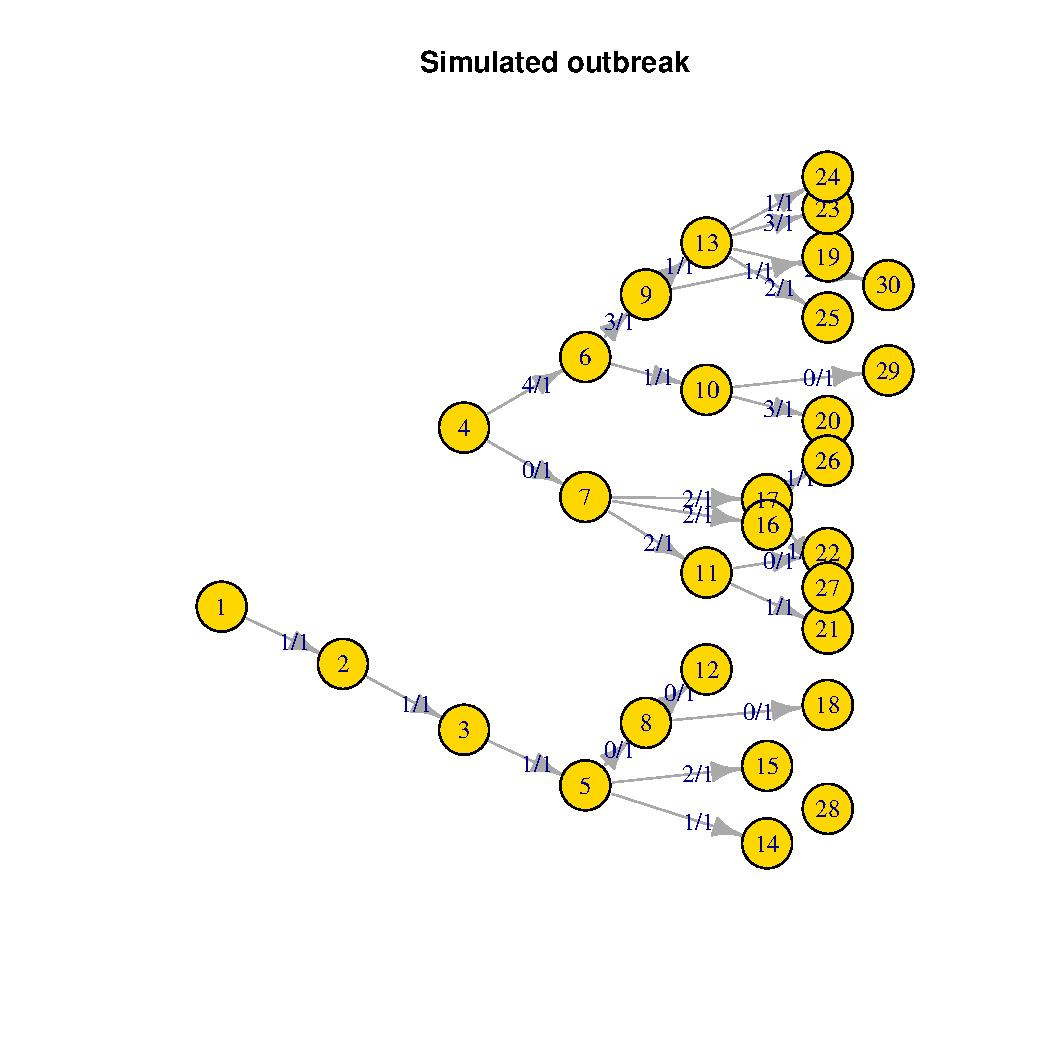
\includegraphics[width=.6\textwidth]{figs/unnamed-chunk-31} 

}


\begin{kframe}\begin{alltt}
\hlkwd{barplot}\hlstd{(w,} \hlkwc{main}\hlstd{=}\hlstr{"Generation time distribution"}\hlstd{,} \hlkwc{ylab}\hlstd{=}\hlstr{"probability"}\hlstd{,} \hlkwc{xlab}\hlstd{=}\hlstr{"days"}\hlstd{,} \hlkwc{names}\hlstd{=}\hlnum{0}\hlopt{:}\hlnum{3}\hlstd{)}
\end{alltt}
\end{kframe}

{\centering 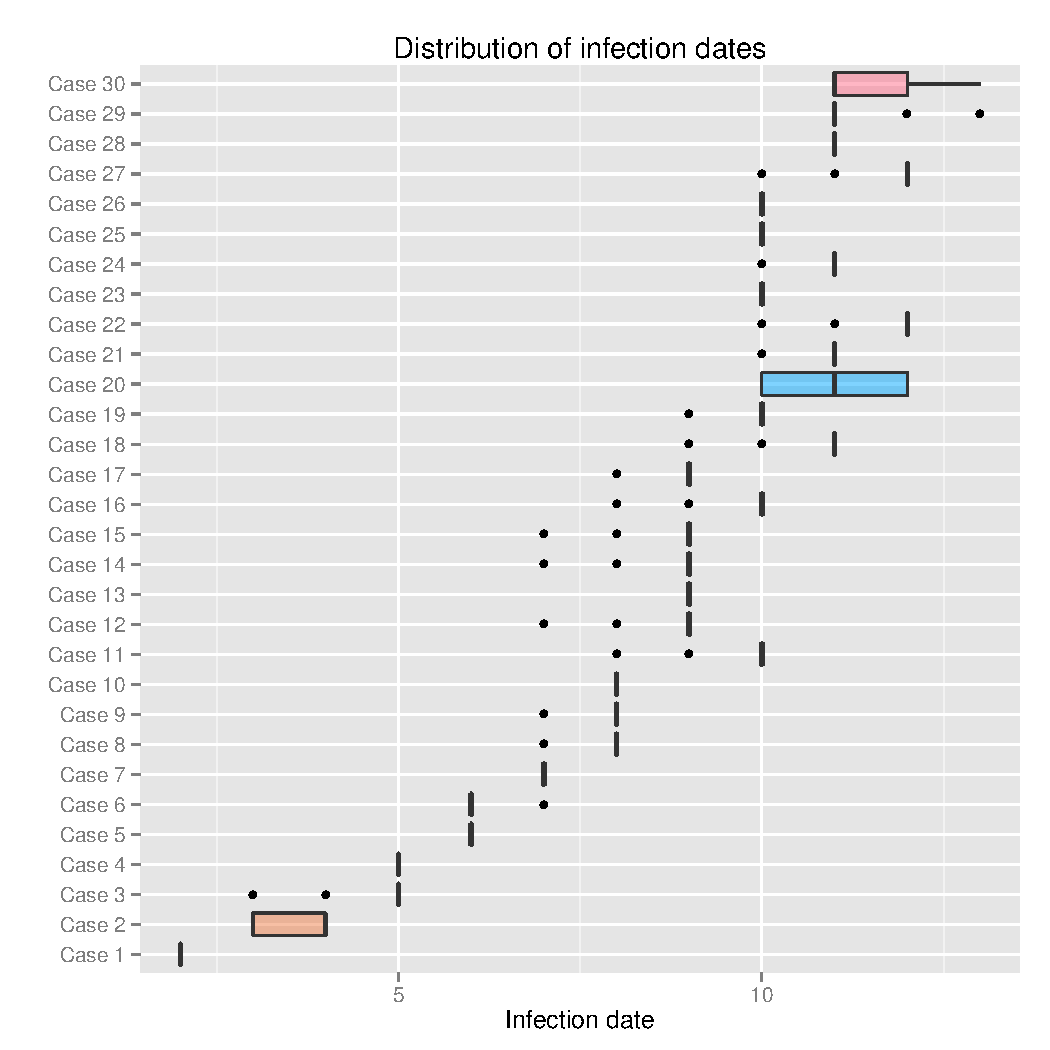
\includegraphics[width=.6\textwidth]{figs/unnamed-chunk-32} 

}



\end{knitrout}




\begin{knitrout}
\definecolor{shadecolor}{rgb}{0.969, 0.969, 0.969}\color{fgcolor}\begin{kframe}
\begin{alltt}
\hlstd{res} \hlkwb{<-}  \hlkwd{outbreaker.parallel}\hlstd{(}\hlkwc{n.runs}\hlstd{=}\hlnum{4}\hlstd{,} \hlkwc{dna}\hlstd{=dat}\hlopt{$}\hlstd{dna,}
                            \hlkwc{dates}\hlstd{=collecDates,}\hlkwc{w.dens}\hlstd{=w,} \hlkwc{n.iter}\hlstd{=}\hlnum{5e4}\hlstd{)}
\end{alltt}
\end{kframe}
\end{knitrout}




\begin{knitrout}
\definecolor{shadecolor}{rgb}{0.969, 0.969, 0.969}\color{fgcolor}\begin{kframe}
\begin{alltt}
\hlkwd{names}\hlstd{(res)}
\end{alltt}
\begin{verbatim}
##  [1] "chains"         "collec.dates"   "w"              "f"             
##  [5] "D"              "idx.dna"        "tune.end"       "find.import"   
##  [9] "burnin"         "find.import.at" "n.runs"         "call"
\end{verbatim}
\end{kframe}
\end{knitrout}


\begin{knitrout}
\definecolor{shadecolor}{rgb}{0.969, 0.969, 0.969}\color{fgcolor}\begin{kframe}
\begin{alltt}
\hlkwd{names}\hlstd{(res}\hlopt{$}\hlstd{chains)}
\end{alltt}
\begin{verbatim}
##   [1] "step"     "post"     "like"     "prior"    "mu1"      "mu2"     
##   [7] "gamma"    "pi"       "spa1"     "spa2"     "Tinf_1"   "Tinf_2"  
##  [13] "Tinf_3"   "Tinf_4"   "Tinf_5"   "Tinf_6"   "Tinf_7"   "Tinf_8"  
##  [19] "Tinf_9"   "Tinf_10"  "Tinf_11"  "Tinf_12"  "Tinf_13"  "Tinf_14" 
##  [25] "Tinf_15"  "Tinf_16"  "Tinf_17"  "Tinf_18"  "Tinf_19"  "Tinf_20" 
##  [31] "Tinf_21"  "Tinf_22"  "Tinf_23"  "Tinf_24"  "Tinf_25"  "Tinf_26" 
##  [37] "Tinf_27"  "Tinf_28"  "Tinf_29"  "Tinf_30"  "alpha_1"  "alpha_2" 
##  [43] "alpha_3"  "alpha_4"  "alpha_5"  "alpha_6"  "alpha_7"  "alpha_8" 
##  [49] "alpha_9"  "alpha_10" "alpha_11" "alpha_12" "alpha_13" "alpha_14"
##  [55] "alpha_15" "alpha_16" "alpha_17" "alpha_18" "alpha_19" "alpha_20"
##  [61] "alpha_21" "alpha_22" "alpha_23" "alpha_24" "alpha_25" "alpha_26"
##  [67] "alpha_27" "alpha_28" "alpha_29" "alpha_30" "kappa_1"  "kappa_2" 
##  [73] "kappa_3"  "kappa_4"  "kappa_5"  "kappa_6"  "kappa_7"  "kappa_8" 
##  [79] "kappa_9"  "kappa_10" "kappa_11" "kappa_12" "kappa_13" "kappa_14"
##  [85] "kappa_15" "kappa_16" "kappa_17" "kappa_18" "kappa_19" "kappa_20"
##  [91] "kappa_21" "kappa_22" "kappa_23" "kappa_24" "kappa_25" "kappa_26"
##  [97] "kappa_27" "kappa_28" "kappa_29" "kappa_30" "run"
\end{verbatim}
\end{kframe}
\end{knitrout}



\begin{knitrout}
\definecolor{shadecolor}{rgb}{0.969, 0.969, 0.969}\color{fgcolor}\begin{kframe}
\begin{alltt}
\hlkwd{class}\hlstd{(res)}
\end{alltt}
\begin{verbatim}
## [1] "list"
\end{verbatim}
\begin{alltt}
\hlkwd{names}\hlstd{(res)}
\end{alltt}
\begin{verbatim}
##  [1] "chains"         "collec.dates"   "w"              "f"             
##  [5] "D"              "idx.dna"        "tune.end"       "find.import"   
##  [9] "burnin"         "find.import.at" "n.runs"         "call"
\end{verbatim}
\end{kframe}
\end{knitrout}

The object \texttt{res} is a list with a number of named items, described in \texttt{?outbreaker}.
The most important one is \texttt{res\$chains}, containing the MCMC outputs:
\begin{knitrout}
\definecolor{shadecolor}{rgb}{0.969, 0.969, 0.969}\color{fgcolor}\begin{kframe}
\begin{alltt}
\hlkwd{class}\hlstd{(res}\hlopt{$}\hlstd{chains)}
\end{alltt}
\begin{verbatim}
## [1] "data.frame"
\end{verbatim}
\begin{alltt}
\hlkwd{dim}\hlstd{(res}\hlopt{$}\hlstd{chains)}
\end{alltt}
\begin{verbatim}
## [1] 804 101
\end{verbatim}
\begin{alltt}
\hlkwd{names}\hlstd{(res}\hlopt{$}\hlstd{chains)}
\end{alltt}
\begin{verbatim}
##   [1] "step"     "post"     "like"     "prior"    "mu1"      "mu2"     
##   [7] "gamma"    "pi"       "spa1"     "spa2"     "Tinf_1"   "Tinf_2"  
##  [13] "Tinf_3"   "Tinf_4"   "Tinf_5"   "Tinf_6"   "Tinf_7"   "Tinf_8"  
##  [19] "Tinf_9"   "Tinf_10"  "Tinf_11"  "Tinf_12"  "Tinf_13"  "Tinf_14" 
##  [25] "Tinf_15"  "Tinf_16"  "Tinf_17"  "Tinf_18"  "Tinf_19"  "Tinf_20" 
##  [31] "Tinf_21"  "Tinf_22"  "Tinf_23"  "Tinf_24"  "Tinf_25"  "Tinf_26" 
##  [37] "Tinf_27"  "Tinf_28"  "Tinf_29"  "Tinf_30"  "alpha_1"  "alpha_2" 
##  [43] "alpha_3"  "alpha_4"  "alpha_5"  "alpha_6"  "alpha_7"  "alpha_8" 
##  [49] "alpha_9"  "alpha_10" "alpha_11" "alpha_12" "alpha_13" "alpha_14"
##  [55] "alpha_15" "alpha_16" "alpha_17" "alpha_18" "alpha_19" "alpha_20"
##  [61] "alpha_21" "alpha_22" "alpha_23" "alpha_24" "alpha_25" "alpha_26"
##  [67] "alpha_27" "alpha_28" "alpha_29" "alpha_30" "kappa_1"  "kappa_2" 
##  [73] "kappa_3"  "kappa_4"  "kappa_5"  "kappa_6"  "kappa_7"  "kappa_8" 
##  [79] "kappa_9"  "kappa_10" "kappa_11" "kappa_12" "kappa_13" "kappa_14"
##  [85] "kappa_15" "kappa_16" "kappa_17" "kappa_18" "kappa_19" "kappa_20"
##  [91] "kappa_21" "kappa_22" "kappa_23" "kappa_24" "kappa_25" "kappa_26"
##  [97] "kappa_27" "kappa_28" "kappa_29" "kappa_30" "run"
\end{verbatim}
\begin{alltt}
\hlstd{res}\hlopt{$}\hlstd{chains[}\hlnum{1}\hlopt{:}\hlnum{10}\hlstd{,}\hlnum{1}\hlopt{:}\hlnum{10}\hlstd{]}
\end{alltt}
\begin{verbatim}
##    step    post    like prior       mu1       mu2 gamma     pi spa1 spa2
## 1     1 -1106.3 -1108.4 2.093 5.000e-05 5.000e-05     1 0.9770    0    0
## 2   500  -468.0  -470.2 2.144 5.021e-05 5.021e-05     1 0.9826    0    0
## 3  1000  -446.9  -448.8 1.909 5.038e-05 5.038e-05     1 0.9572    0    0
## 4  1500  -446.7  -448.9 2.294 5.060e-05 5.060e-05     1 0.9990    0    0
## 5  2000  -446.5  -448.7 2.227 5.087e-05 5.087e-05     1 0.9916    0    0
## 6  2500  -446.6  -448.7 2.147 5.080e-05 5.080e-05     1 0.9829    0    0
## 7  3000  -446.9  -449.1 2.216 5.138e-05 5.138e-05     1 0.9905    0    0
## 8  3500  -448.5  -450.6 2.168 5.078e-05 5.078e-05     1 0.9852    0    0
## 9  4000  -446.8  -449.1 2.233 5.309e-05 5.309e-05     1 0.9923    0    0
## 10 4500  -452.0  -453.8 1.855 5.323e-05 5.323e-05     1 0.9515    0    0
\end{verbatim}
\end{kframe}
\end{knitrout}

The columns of this \texttt{data.frame} store the following outputs:
\begin{itemize}
  \item \texttt{step}: the MCMC iteration of the sample
  \item \texttt{post/like/prior}: log values for posterior, likelihood, and prior densities
  \item \texttt{mu1}: in mutation model 1, mutation rate; otherwise, the rate of transitions, per site and generation
  \item \texttt{mu2}: in mutation model 1, mutation rate (mu1=mu2); otherwise, the rate of transversions, per site and generation
  \item \texttt{gamma}: the ratio between transversions and transitions ($\mu_2 / \mu_1$)
  \item \texttt{pi}: the proportion of the transmission tree sampled
  \item \texttt{Tinf\_[}\textit{number}\texttt{]}: dates of infection
  \item \texttt{alpha\_[}\textit{number}\texttt{]}: the index of the ancestral cases (infectors)
  \item \texttt{kappa\_[}\textit{number}\texttt{]}: the number of generations between cases and
    their most recent sampled ancestor (here, fixed to 1)
  \item \texttt{run}: for parallel runs, the index of the run.
\end{itemize}





%%%%%%%%%%%%%%%%%%%%%%%%%%%%%%%%%%%%%%%%%%%%%%%%%%%%
\subsection{Assessing convergence and determining the burnin}
%%%%%%%%%%%%%%%%%%%%%%%%%%%%%%%%%%%%%%%%%%%%%%%%%%%%

A MCMC is said to converge when it reaches a stationary state, i.e. its distributional properties a
constant over time (mean and variance don't depend on which iteration you consider).
Convergence of the chains is best assessed by comparing parallel runs.
This can be done using \texttt{plotChains}:

\begin{knitrout}
\definecolor{shadecolor}{rgb}{0.969, 0.969, 0.969}\color{fgcolor}\begin{kframe}
\begin{alltt}
\hlkwd{plotChains}\hlstd{(res,} \hlkwc{main}\hlstd{=}\hlstr{"Trace of log-posterior values"}\hlstd{)}
\end{alltt}
\end{kframe}

{\centering 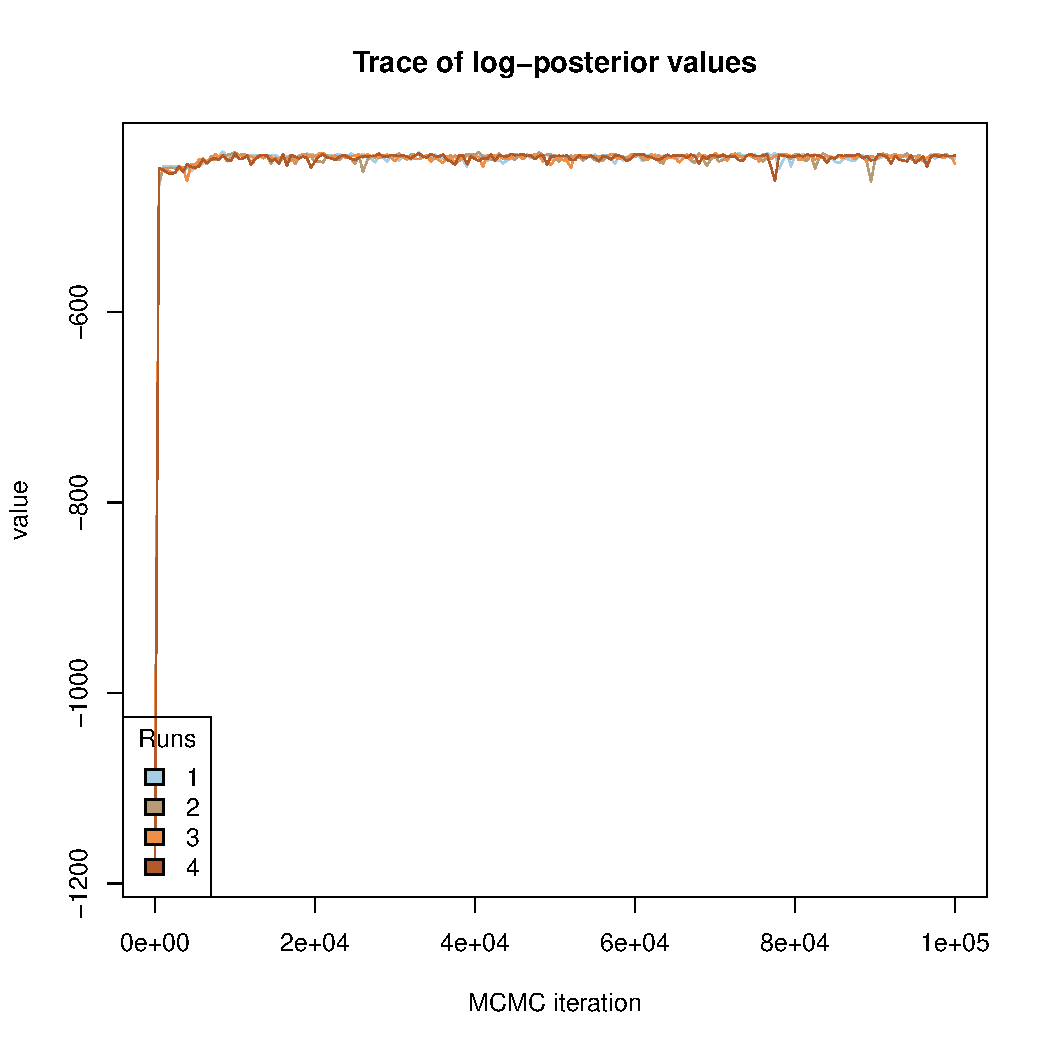
\includegraphics[width=.6\textwidth]{figs/unnamed-chunk-101} 

}


\begin{kframe}\begin{alltt}
\hlkwd{plotChains}\hlstd{(res,} \hlkwc{main}\hlstd{=}\hlstr{"Trace of log-posterior values \textbackslash{}n(burnin removed)"}\hlstd{,}
           \hlkwc{burnin}\hlstd{=}\hlnum{2e4}\hlstd{)}
\end{alltt}
\end{kframe}

{\centering 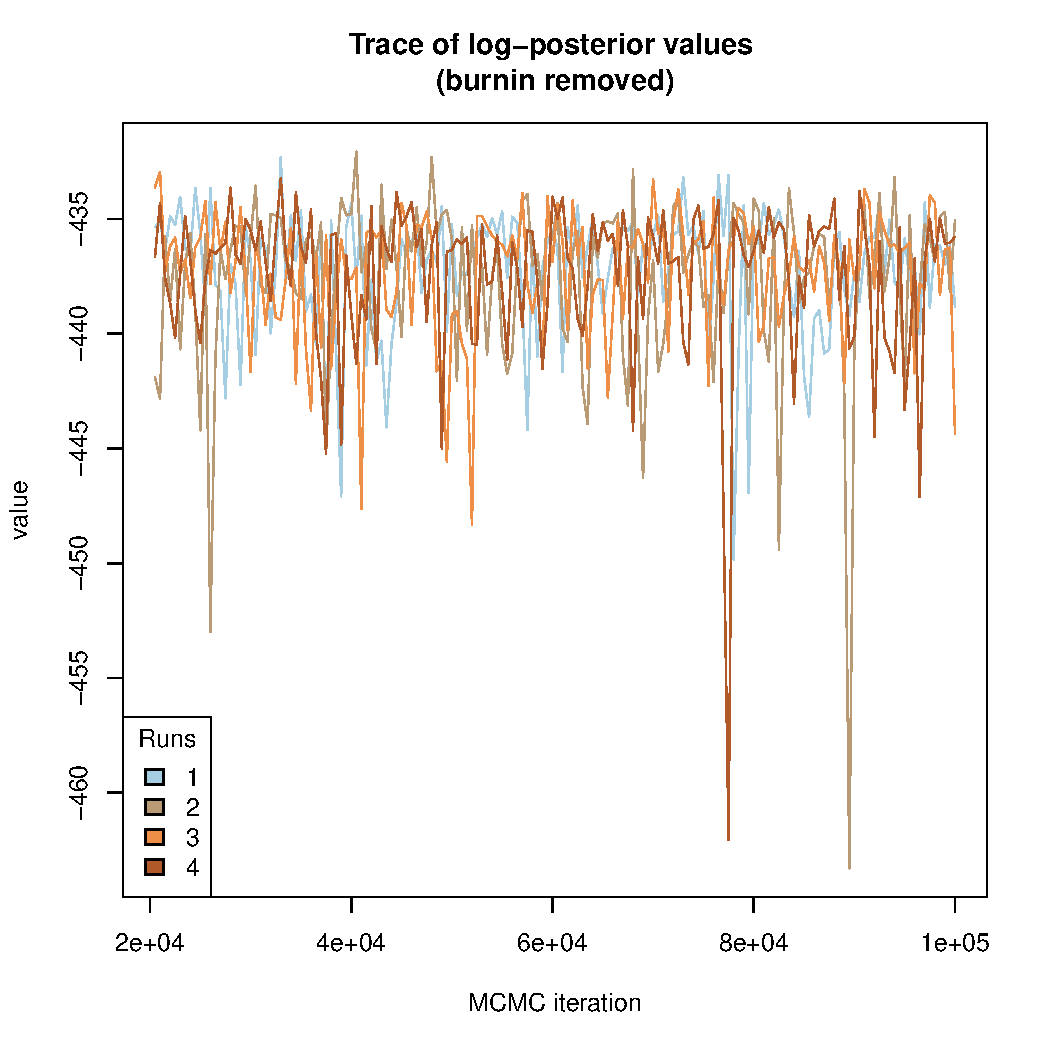
\includegraphics[width=.6\textwidth]{figs/unnamed-chunk-102} 

}


\begin{kframe}\begin{alltt}
\hlkwd{plotChains}\hlstd{(res,} \hlkwc{main}\hlstd{=}\hlstr{"Density log-posterior values \textbackslash{}n(burnin removed)"}\hlstd{,}
           \hlkwc{burnin}\hlstd{=}\hlnum{2e4}\hlstd{,} \hlkwc{type}\hlstd{=}\hlstr{"dens"}\hlstd{)}
\end{alltt}
\end{kframe}

{\centering 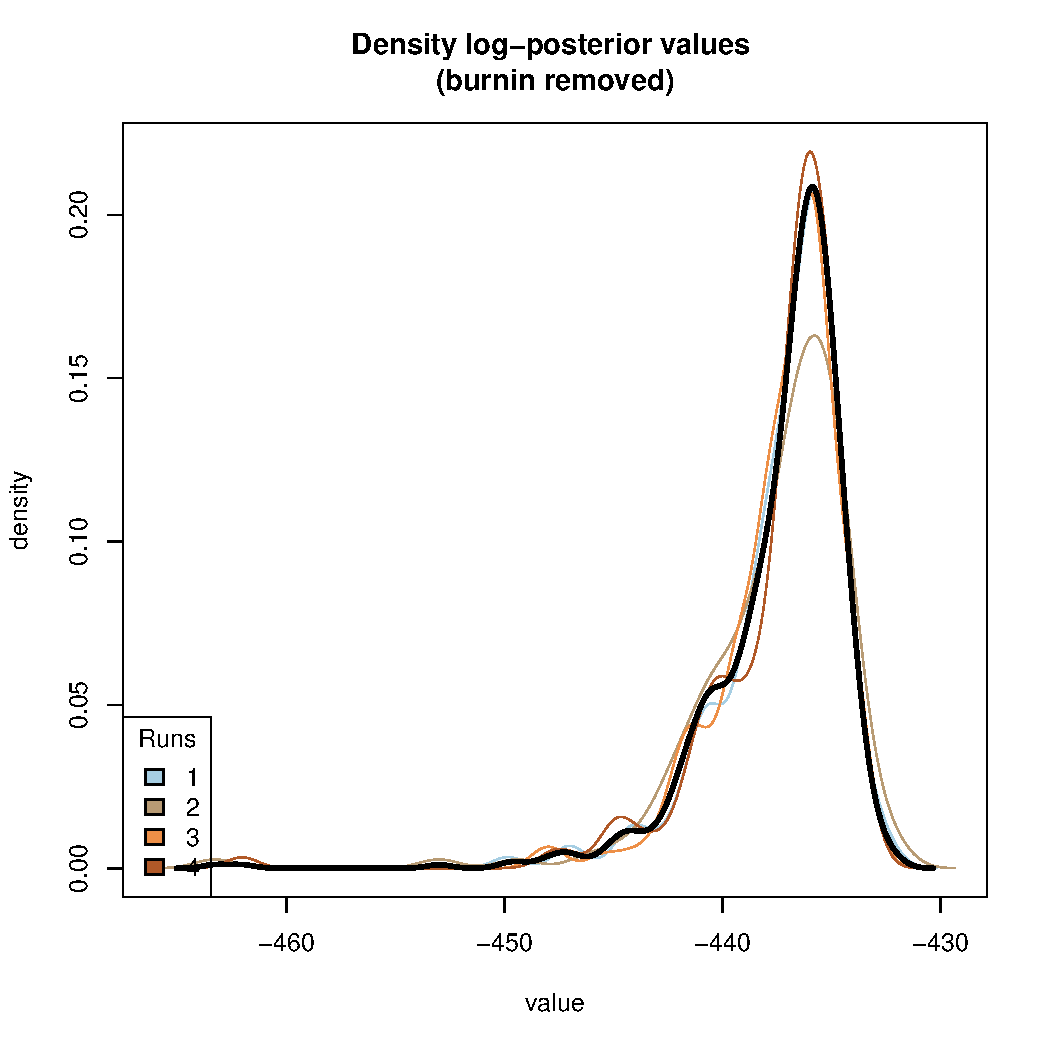
\includegraphics[width=.6\textwidth]{figs/unnamed-chunk-103} 

}



\end{knitrout}




\begin{knitrout}
\definecolor{shadecolor}{rgb}{0.969, 0.969, 0.969}\color{fgcolor}\begin{kframe}
\begin{alltt}
\hlkwd{library}\hlstd{(ggplot2)}
\hlkwd{library}\hlstd{(reshape2)}
\hlstd{x} \hlkwb{<-} \hlstd{res}\hlopt{$}\hlstd{chains}
\hlstd{x}\hlopt{$}\hlstd{run} \hlkwb{<-} \hlkwd{factor}\hlstd{(x}\hlopt{$}\hlstd{run)}
\end{alltt}
\end{kframe}
\end{knitrout}


\begin{knitrout}
\definecolor{shadecolor}{rgb}{0.969, 0.969, 0.969}\color{fgcolor}\begin{kframe}
\begin{alltt}
\hlstd{p} \hlkwb{<-} \hlkwd{ggplot}\hlstd{(x,} \hlkwd{aes}\hlstd{(}\hlkwc{x}\hlstd{=step))} \hlopt{+}
    \hlkwd{geom_line}\hlstd{(}\hlkwd{aes}\hlstd{(}\hlkwc{y}\hlstd{=post,} \hlkwc{colour}\hlstd{=run))} \hlopt{+}
    \hlkwd{labs}\hlstd{(}\hlkwc{title}\hlstd{=}\hlstr{"Trace of log-posterior"}\hlstd{,} \hlkwc{y}\hlstd{=}\hlstr{"log-posterior"}\hlstd{)}
\hlstd{p}
\end{alltt}
\end{kframe}

{\centering 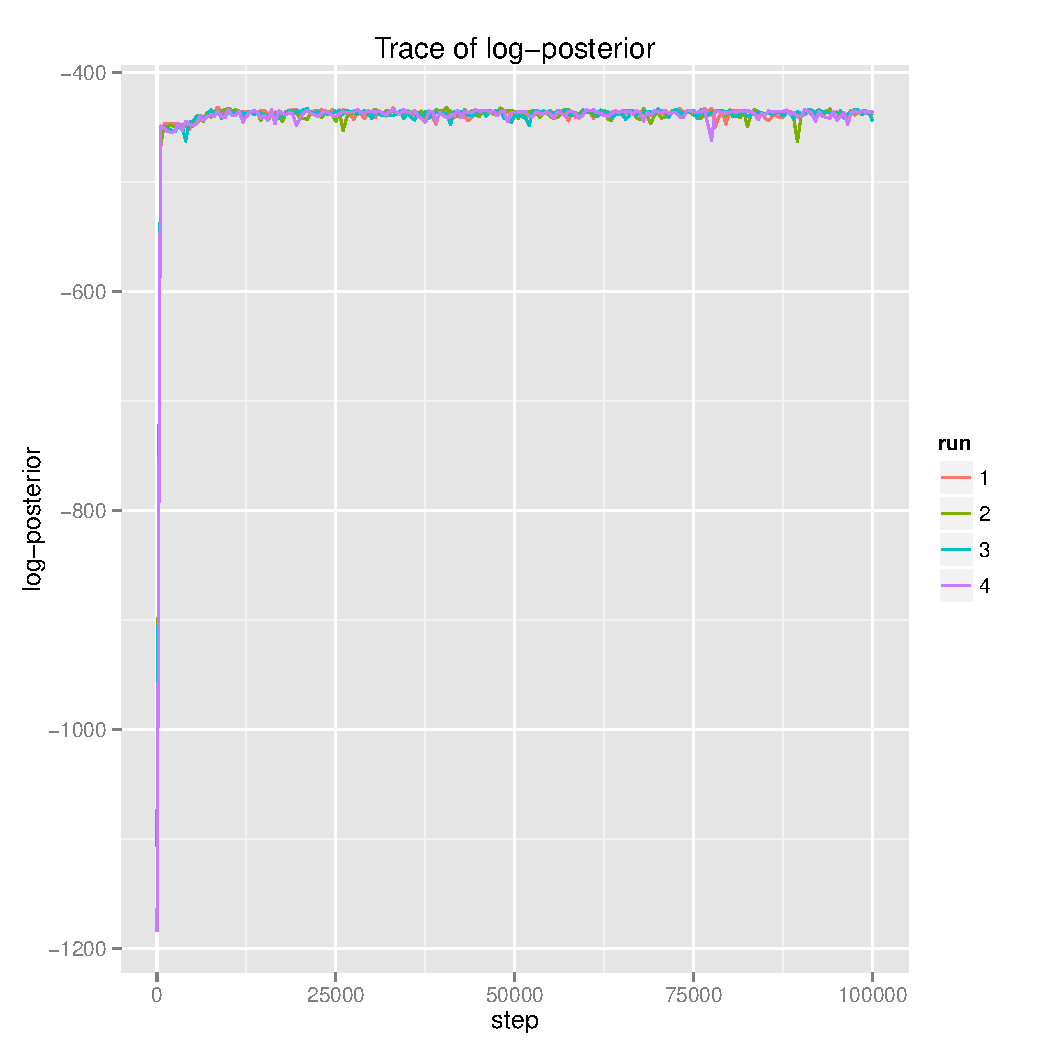
\includegraphics[width=.6\textwidth]{figs/unnamed-chunk-12} 

}



\end{knitrout}

\begin{knitrout}
\definecolor{shadecolor}{rgb}{0.969, 0.969, 0.969}\color{fgcolor}\begin{kframe}
\begin{alltt}
\hlstd{p} \hlopt{+} \hlkwd{scale_y_continuous}\hlstd{(}\hlkwc{limits}\hlstd{=}\hlkwd{c}\hlstd{(}\hlopt{-}\hlnum{460}\hlstd{,}\hlopt{-}\hlnum{430}\hlstd{))}
\end{alltt}
\end{kframe}

{\centering 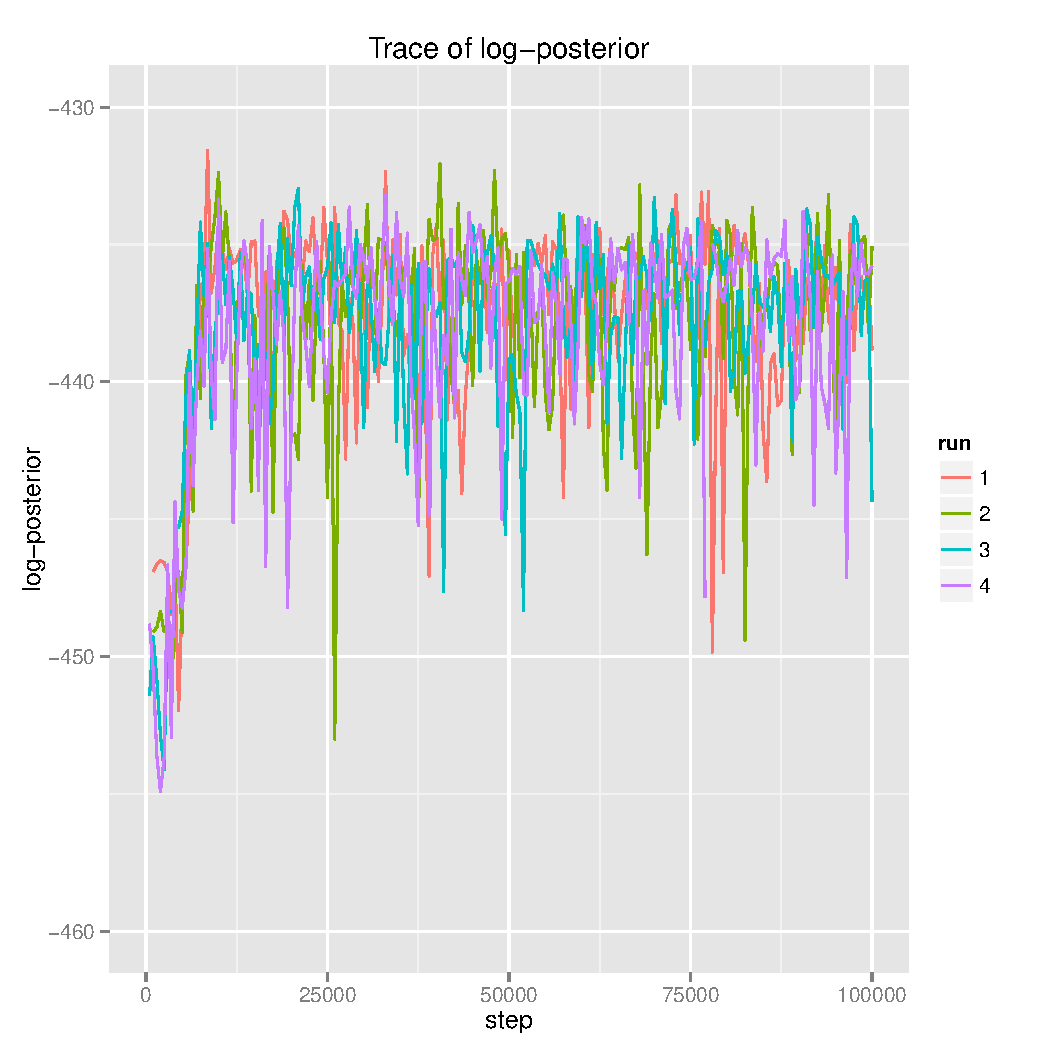
\includegraphics[width=.6\textwidth]{figs/unnamed-chunk-13} 

}



\end{knitrout}


\begin{knitrout}
\definecolor{shadecolor}{rgb}{0.969, 0.969, 0.969}\color{fgcolor}\begin{kframe}
\begin{alltt}
\hlstd{p} \hlopt{+} \hlkwd{scale_y_continuous}\hlstd{(}\hlkwc{limits}\hlstd{=}\hlkwd{c}\hlstd{(}\hlopt{-}\hlnum{460}\hlstd{,}\hlopt{-}\hlnum{430}\hlstd{))} \hlopt{+} \hlkwd{geom_smooth}\hlstd{(}\hlkwd{aes}\hlstd{(}\hlkwc{y}\hlstd{=post))}
\end{alltt}


{\ttfamily\noindent\itshape\color{messagecolor}{\#\# geom\_smooth: method="{}auto"{} and size of largest group is <1000, so using loess. Use 'method = x' to change the smoothing method.}}\end{kframe}

{\centering 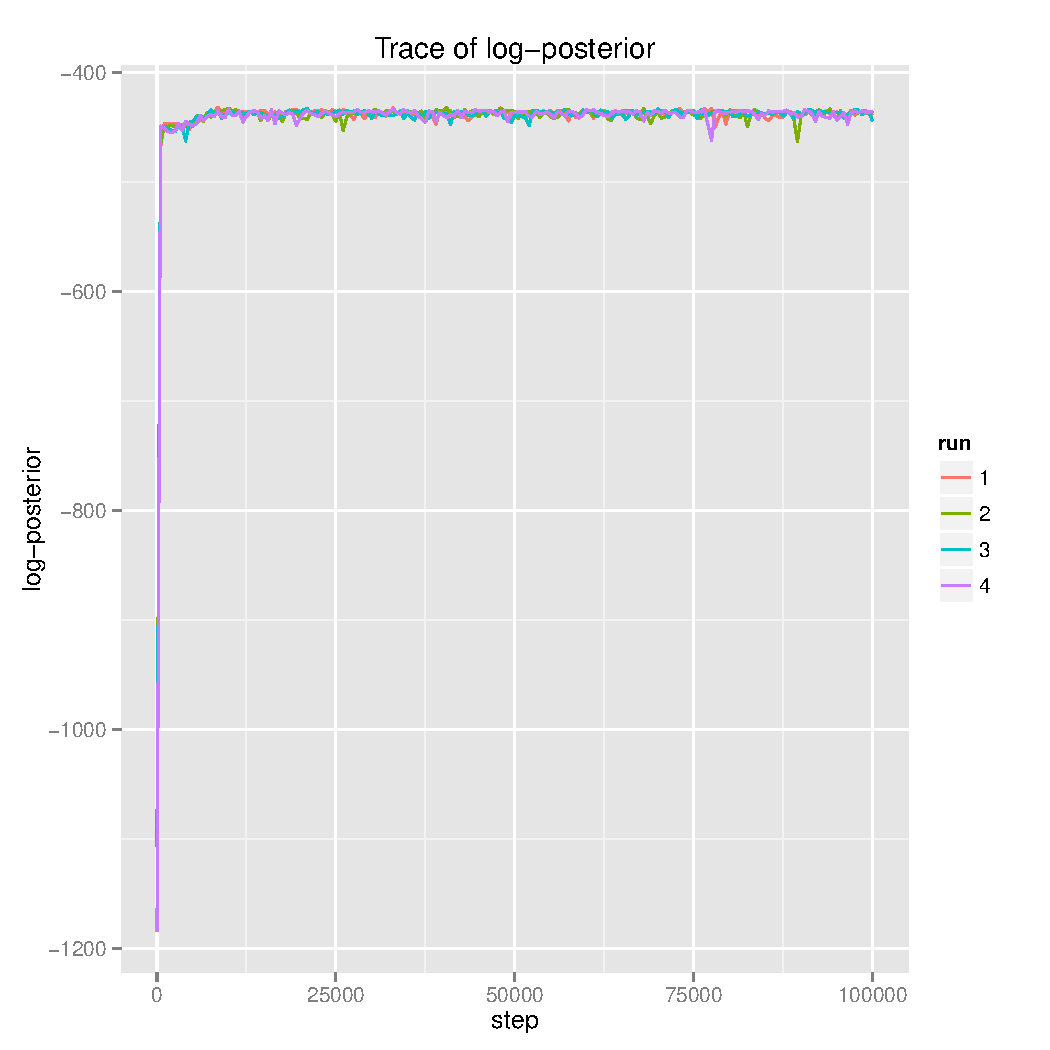
\includegraphics[width=.6\textwidth]{figs/unnamed-chunk-14} 

}



\end{knitrout}



\begin{knitrout}
\definecolor{shadecolor}{rgb}{0.969, 0.969, 0.969}\color{fgcolor}\begin{kframe}
\begin{alltt}
\hlstd{p} \hlkwb{<-} \hlkwd{ggplot}\hlstd{(}\hlkwc{data}\hlstd{=x)} \hlopt{+} \hlkwd{labs}\hlstd{(}\hlkwc{title}\hlstd{=}\hlstr{"Distribution of log-posterior values"}\hlstd{,} \hlkwc{x}\hlstd{=}\hlstr{"log-posterior"}\hlstd{)} \hlopt{+}
    \hlkwd{scale_x_continuous}\hlstd{(}\hlkwc{limits}\hlstd{=}\hlkwd{c}\hlstd{(}\hlopt{-}\hlnum{460}\hlstd{,}\hlopt{-}\hlnum{430}\hlstd{))}
\hlstd{p} \hlopt{+} \hlkwd{geom_density}\hlstd{(}\hlkwd{aes}\hlstd{(}\hlkwc{x}\hlstd{=post,} \hlkwc{fill}\hlstd{=run),} \hlkwc{alpha}\hlstd{=}\hlnum{.3}\hlstd{,} \hlkwc{colour}\hlstd{=}\hlnum{NA}\hlstd{)} \hlopt{+}
    \hlkwd{geom_density}\hlstd{(}\hlkwd{aes}\hlstd{(}\hlkwc{x}\hlstd{=post),} \hlkwc{size}\hlstd{=}\hlnum{1}\hlstd{,} \hlkwc{colour}\hlstd{=}\hlstr{"black"}\hlstd{,} \hlkwc{shape}\hlstd{=}\hlnum{2}\hlstd{,} \hlkwc{alpha}\hlstd{=}\hlnum{.8}\hlstd{)}
\end{alltt}
\end{kframe}

{\centering 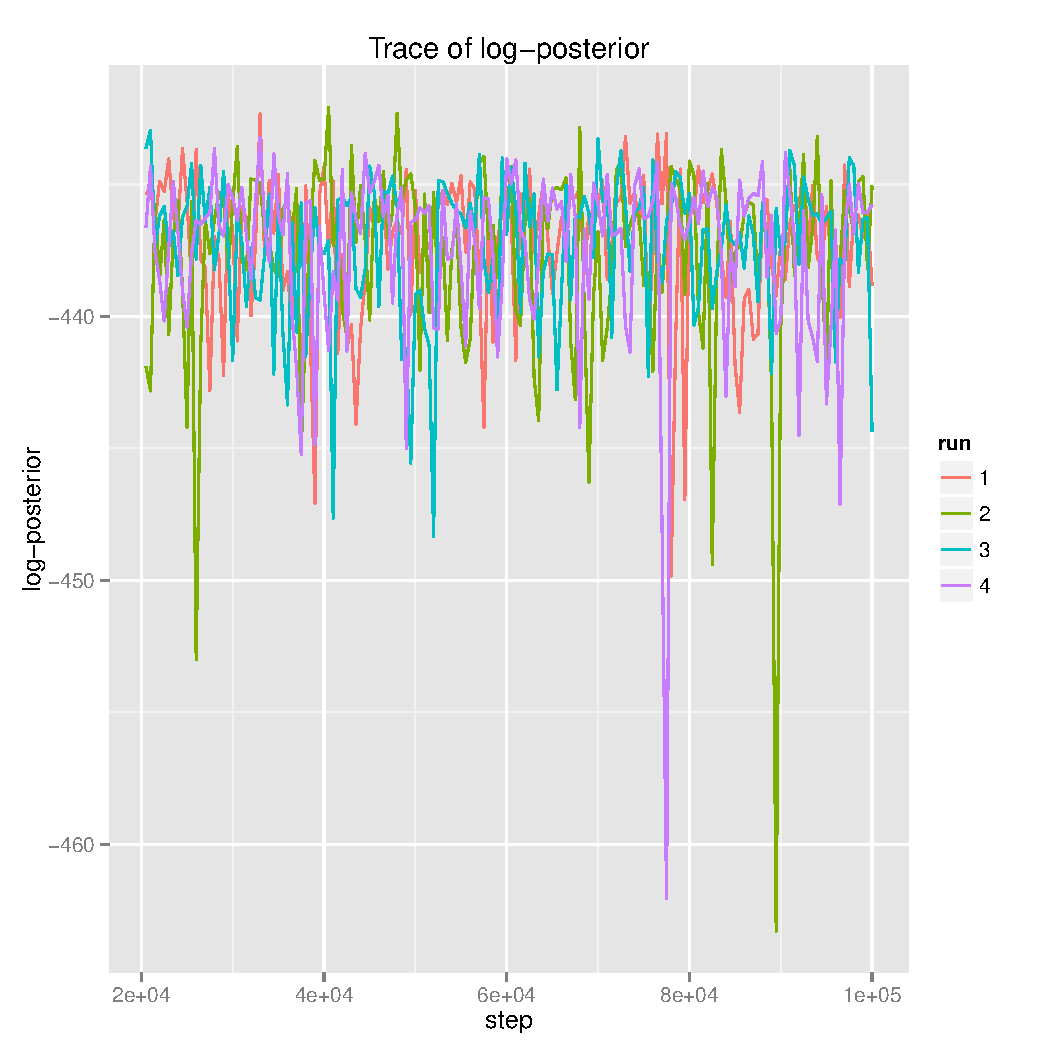
\includegraphics[width=.6\textwidth]{figs/unnamed-chunk-15} 

}



\end{knitrout}


\begin{knitrout}
\definecolor{shadecolor}{rgb}{0.969, 0.969, 0.969}\color{fgcolor}\begin{kframe}
\begin{alltt}
\hlstd{p} \hlopt{+} \hlkwd{geom_histogram}\hlstd{(}\hlkwd{aes}\hlstd{(}\hlkwc{x}\hlstd{=post,} \hlkwc{fill}\hlstd{=run,} \hlkwc{y}\hlstd{=..density..),} \hlkwc{alpha}\hlstd{=}\hlnum{.7}\hlstd{,} \hlkwc{colour}\hlstd{=}\hlnum{NA}\hlstd{,} \hlkwc{position}\hlstd{=}\hlstr{"dodge"}\hlstd{)} \hlopt{+}
    \hlkwd{geom_density}\hlstd{(}\hlkwd{aes}\hlstd{(}\hlkwc{x}\hlstd{=post),} \hlkwc{size}\hlstd{=}\hlnum{1}\hlstd{,} \hlkwc{colour}\hlstd{=}\hlstr{"black"}\hlstd{,} \hlkwc{shape}\hlstd{=}\hlnum{2}\hlstd{,} \hlkwc{alpha}\hlstd{=}\hlnum{.8}\hlstd{)}
\end{alltt}


{\ttfamily\noindent\itshape\color{messagecolor}{\#\# stat\_bin: binwidth defaulted to range/30. Use 'binwidth = x' to adjust this.}}\end{kframe}

{\centering 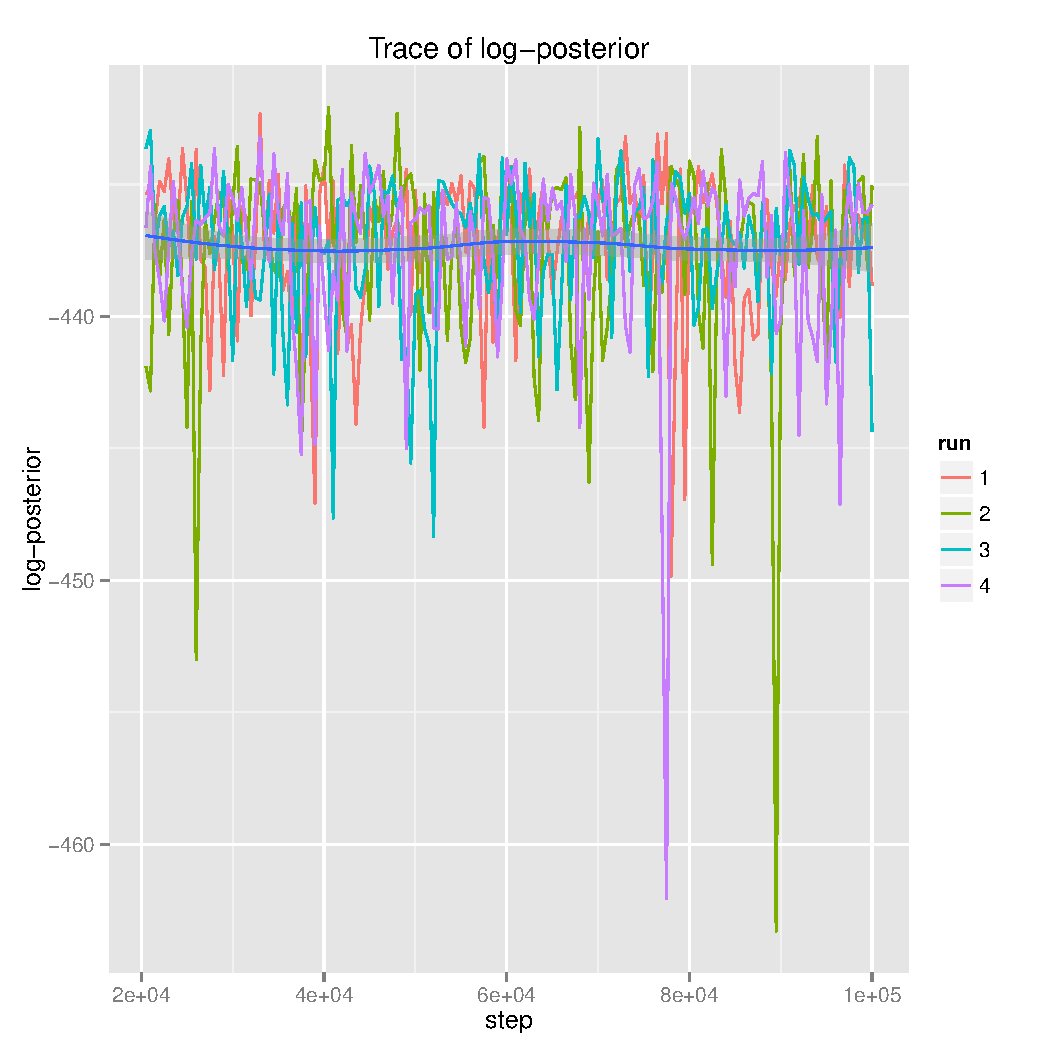
\includegraphics[width=.6\textwidth]{figs/unnamed-chunk-16} 

}



\end{knitrout}







%%%%%%%%%%%%%%%%%%%%%%%%%%%%%%%%%%%%%%%%%%%%%%%%%%%%
%%%%%%%%%%%%%%%%%%%%%%%%%%%%%%%%%%%%%%%%%%%%%%%%%%%%
\section{Interpreting the results}
%%%%%%%%%%%%%%%%%%%%%%%%%%%%%%%%%%%%%%%%%%%%%%%%%%%%
%%%%%%%%%%%%%%%%%%%%%%%%%%%%%%%%%%%%%%%%%%%%%%%%%%%%

%%%%%%%%%%%%%%%%%%%%%%%%%%%%%%%%%%%%%%%%%%%%%%%%%%%%
\subsection{Visualizing reconstructed transmission trees}
%%%%%%%%%%%%%%%%%%%%%%%%%%%%%%%%%%%%%%%%%%%%%%%%%%%%

\begin{knitrout}
\definecolor{shadecolor}{rgb}{0.969, 0.969, 0.969}\color{fgcolor}\begin{kframe}
\begin{alltt}
\hlkwd{library}\hlstd{(igraph)}
\hlkwd{library}\hlstd{(adegenet)}
\end{alltt}
\end{kframe}
\end{knitrout}

\begin{knitrout}
\definecolor{shadecolor}{rgb}{0.969, 0.969, 0.969}\color{fgcolor}\begin{kframe}
\begin{alltt}
\hlstd{g} \hlkwb{<-} \hlkwd{transGraph}\hlstd{(res,} \hlkwc{thres}\hlstd{=}\hlnum{0}\hlstd{)}
\end{alltt}
\end{kframe}

{\centering 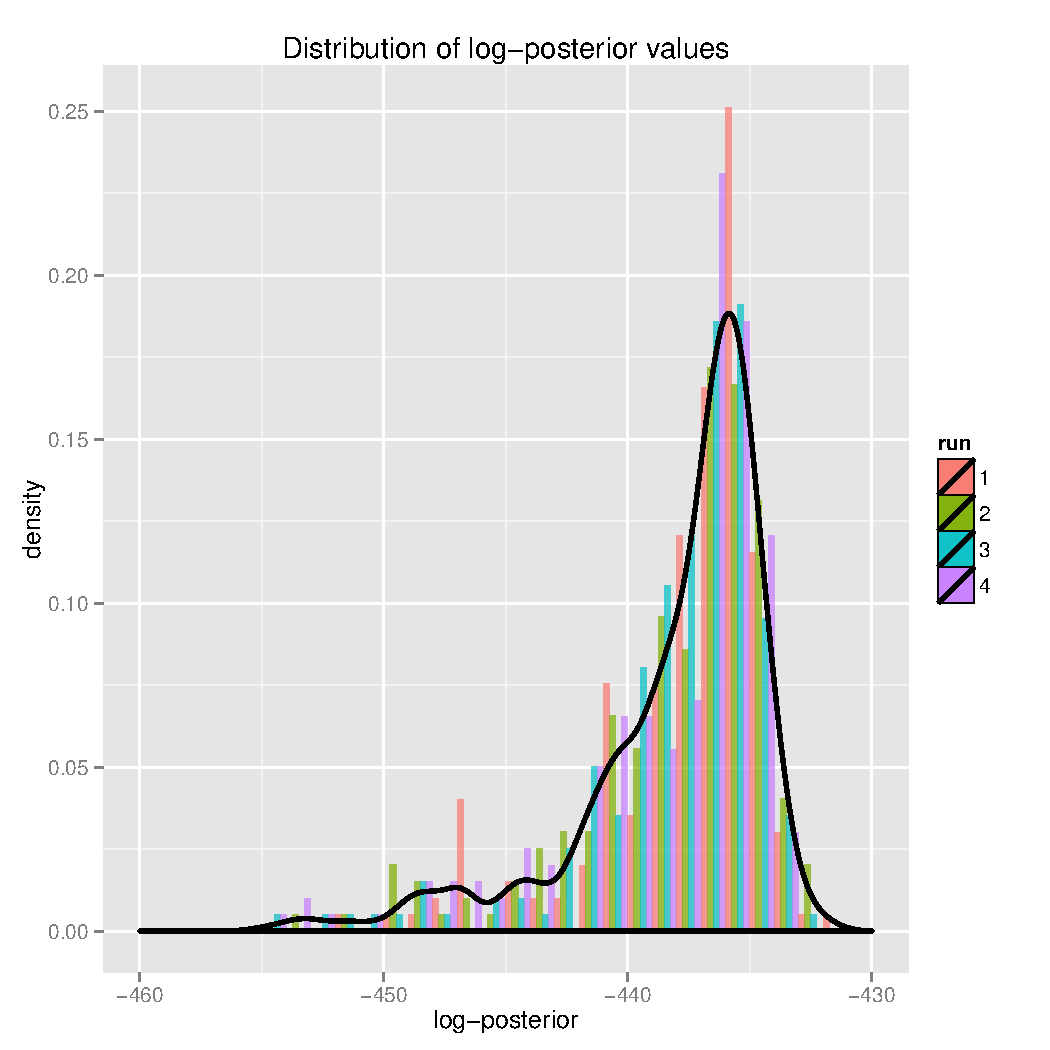
\includegraphics[width=.6\textwidth]{figs/unnamed-chunk-18} 

}



\end{knitrout}



\begin{knitrout}
\definecolor{shadecolor}{rgb}{0.969, 0.969, 0.969}\color{fgcolor}\begin{kframe}
\begin{alltt}
\hlkwd{plot}\hlstd{(g,} \hlkwc{layout}\hlstd{=layout.circle,} \hlkwc{edge.curved}\hlstd{=}\hlnum{FALSE}\hlstd{,} \hlkwc{vertex.color}\hlstd{=}\hlkwd{funky}\hlstd{(}\hlnum{30}\hlstd{))}
\end{alltt}
\end{kframe}

{\centering 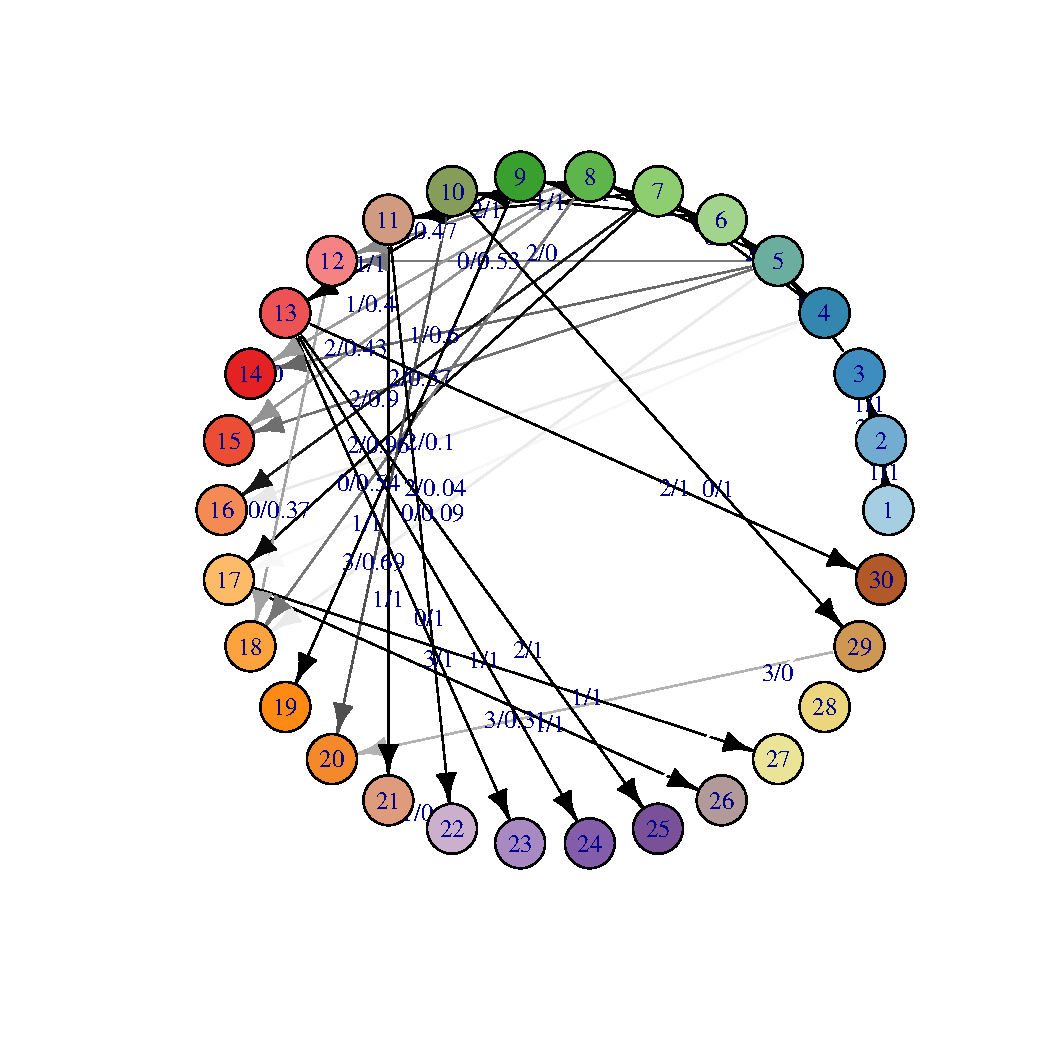
\includegraphics[width=.6\textwidth]{figs/unnamed-chunk-19} 

}



\end{knitrout}



\begin{knitrout}
\definecolor{shadecolor}{rgb}{0.969, 0.969, 0.969}\color{fgcolor}\begin{kframe}
\begin{alltt}
\hlstd{g} \hlkwb{<-} \hlkwd{transGraph}\hlstd{(res,} \hlkwc{thres}\hlstd{=}\hlnum{0.5}\hlstd{,} \hlkwc{annot}\hlstd{=}\hlstr{""}\hlstd{)}
\end{alltt}
\end{kframe}

{\centering 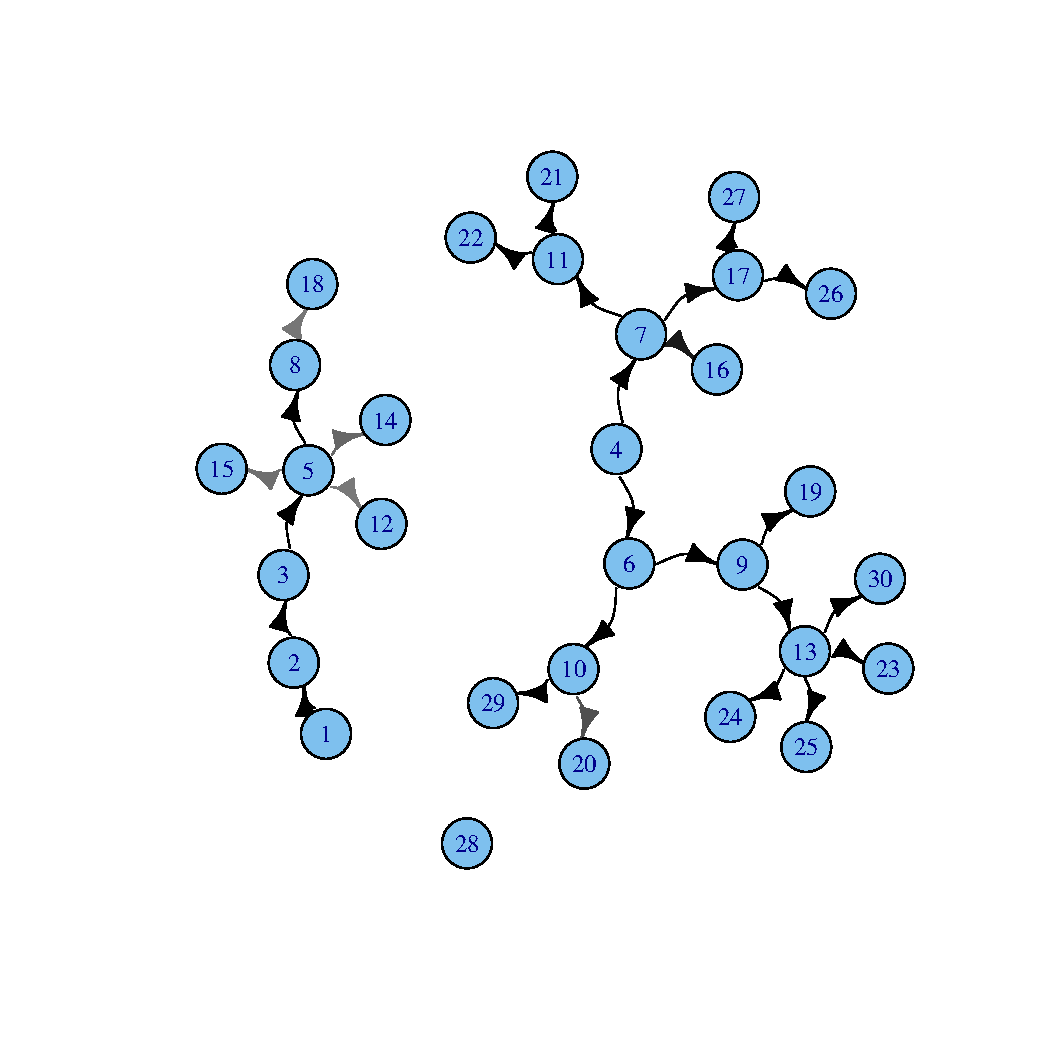
\includegraphics[width=.6\textwidth]{figs/unnamed-chunk-201} 

}


\begin{kframe}\begin{alltt}
\hlstd{edge.colors} \hlkwb{<-} \hlkwd{funky}\hlstd{(}\hlnum{30}\hlstd{)[}\hlkwd{as.numeric}\hlstd{(}\hlkwd{get.edgelist}\hlstd{(g)[,}\hlnum{1}\hlstd{])]}
\hlkwd{plot}\hlstd{(g,} \hlkwc{layout}\hlstd{=layout.circle,} \hlkwc{edge.curved}\hlstd{=}\hlnum{FALSE}\hlstd{,} \hlkwc{vertex.color}\hlstd{=}\hlkwd{funky}\hlstd{(}\hlnum{30}\hlstd{),}
     \hlkwc{edge.color}\hlstd{=edge.colors)}
\hlkwd{title}\hlstd{(}\hlstr{"Ancestries with support >50% - circular graph"}\hlstd{)}
\end{alltt}
\end{kframe}

{\centering 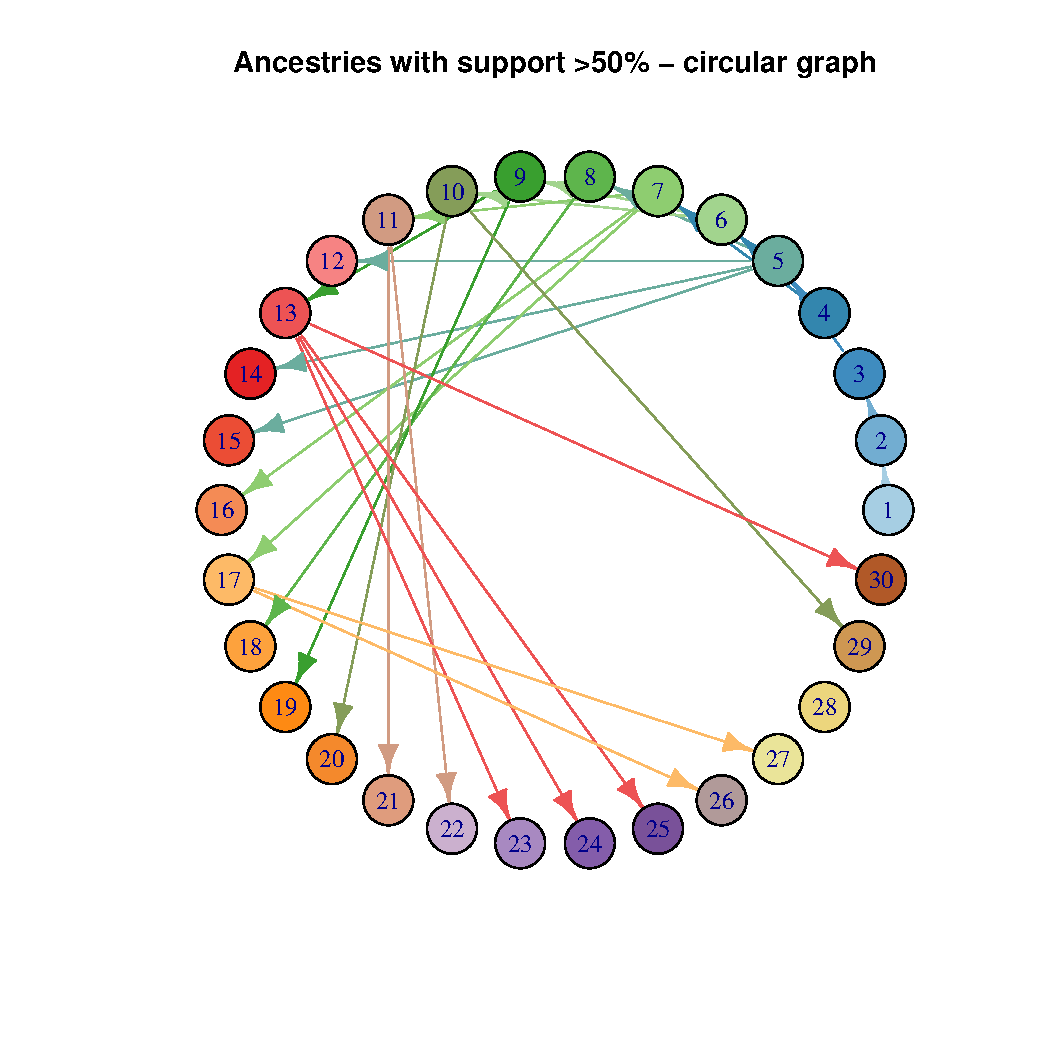
\includegraphics[width=.6\textwidth]{figs/unnamed-chunk-202} 

}


\begin{kframe}\begin{alltt}
\hlkwd{plot}\hlstd{(g,} \hlkwc{layout}\hlstd{=layout.auto,} \hlkwc{edge.curved}\hlstd{=}\hlnum{FALSE}\hlstd{,} \hlkwc{vertex.color}\hlstd{=}\hlkwd{funky}\hlstd{(}\hlnum{30}\hlstd{),}
     \hlkwc{edge.color}\hlstd{=edge.colors)}
\hlkwd{title}\hlstd{(}\hlstr{"Ancestries with support >50% - other layout"}\hlstd{)}
\end{alltt}
\end{kframe}

{\centering 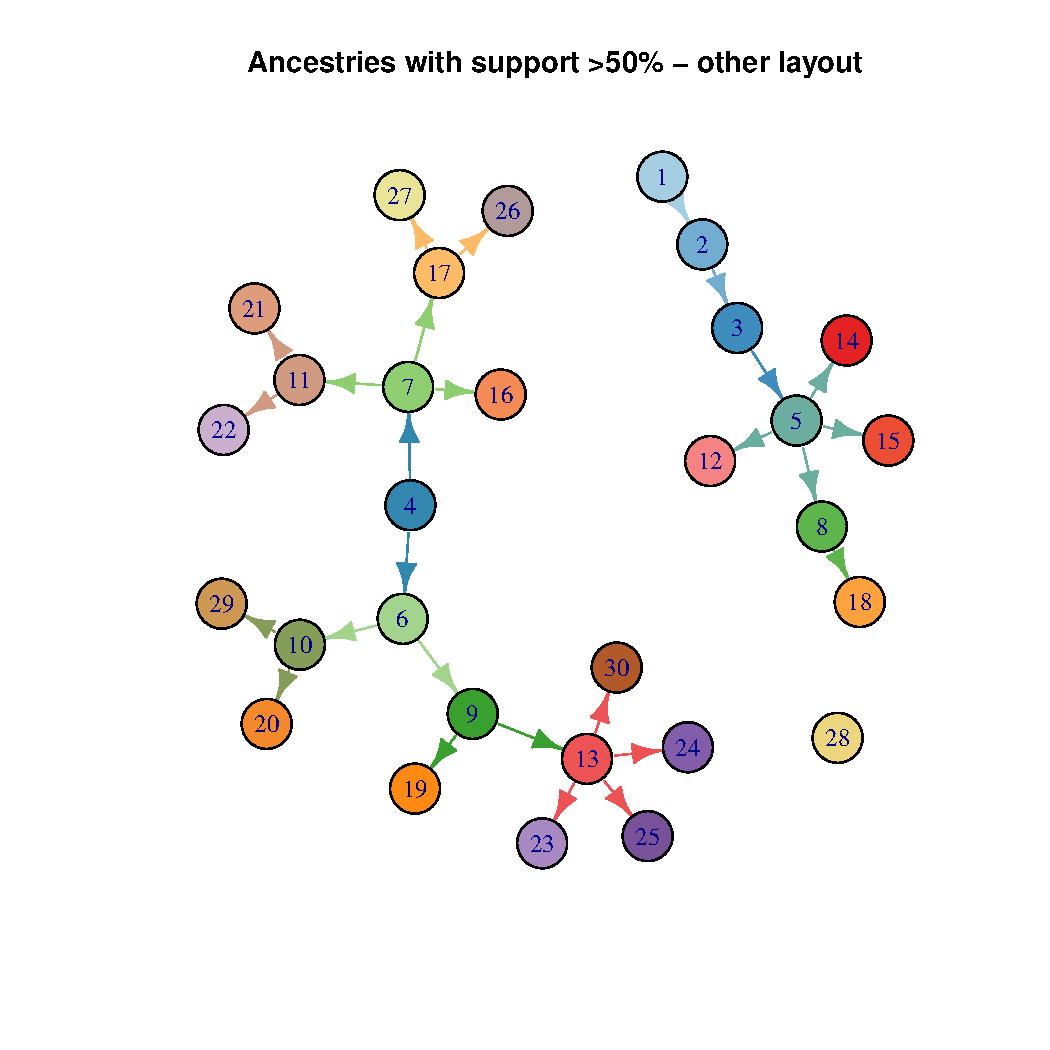
\includegraphics[width=.6\textwidth]{figs/unnamed-chunk-203} 

}



\end{knitrout}


\begin{knitrout}
\definecolor{shadecolor}{rgb}{0.969, 0.969, 0.969}\color{fgcolor}\begin{kframe}
\begin{alltt}
\hlstd{case.size} \hlkwb{<-} \hlnum{10}\hlopt{+}\hlkwd{apply}\hlstd{(}\hlkwd{get.R}\hlstd{(res),}\hlnum{2}\hlstd{,mean)}\hlopt{*}\hlnum{5}
\hlkwd{plot}\hlstd{(g,} \hlkwc{layout}\hlstd{=layout.auto,} \hlkwc{edge.curved}\hlstd{=}\hlnum{FALSE}\hlstd{,} \hlkwc{vertex.color}\hlstd{=}\hlkwd{funky}\hlstd{(}\hlnum{30}\hlstd{),}
     \hlkwc{edge.color}\hlstd{=edge.colors,} \hlkwc{vertex.size}\hlstd{=case.size)}
\hlkwd{title}\hlstd{(}\hlstr{"Ancestries with support >50% \textbackslash{}n(node size reflects R)"}\hlstd{)}
\end{alltt}
\end{kframe}

{\centering 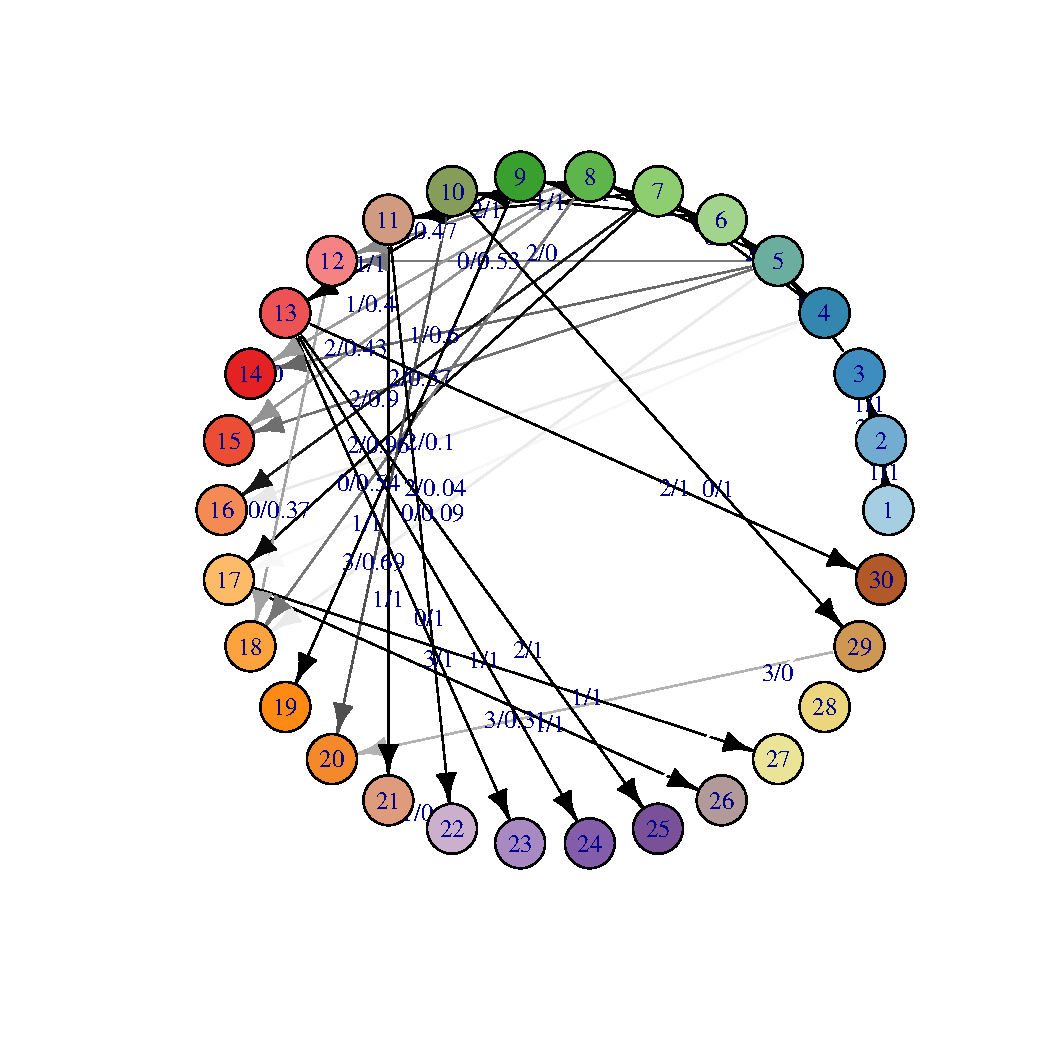
\includegraphics[width=.6\textwidth]{figs/unnamed-chunk-21} 

}



\end{knitrout}



\begin{knitrout}
\definecolor{shadecolor}{rgb}{0.969, 0.969, 0.969}\color{fgcolor}\begin{kframe}
\begin{alltt}
\hlstd{Tinf} \hlkwb{<-} \hlstd{x[x}\hlopt{$}\hlstd{step}\hlopt{>=}\hlnum{2e4}\hlstd{,}\hlkwd{grep}\hlstd{(}\hlstr{"Tinf"}\hlstd{,} \hlkwd{names}\hlstd{(x))]}
\hlstd{case.color} \hlkwb{<-} \hlkwd{any2col}\hlstd{(}\hlkwd{apply}\hlstd{(Tinf,}\hlnum{2}\hlstd{,mean),} \hlkwc{col.pal}\hlstd{=spectral)}
\hlkwd{plot}\hlstd{(g,} \hlkwc{layout}\hlstd{=layout.auto,} \hlkwc{edge.curved}\hlstd{=}\hlnum{FALSE}\hlstd{,} \hlkwc{vertex.color}\hlstd{=case.color}\hlopt{$}\hlstd{col,}
     \hlkwc{vertex.size}\hlstd{=case.size)}
\hlkwd{title}\hlstd{(}\hlstr{"Ancestries with support >50% \textbackslash{}n(node size reflects R)"}\hlstd{)}
\hlkwd{legend}\hlstd{(}\hlstr{"bottomleft"}\hlstd{,} \hlkwc{col}\hlstd{=case.color}\hlopt{$}\hlstd{leg.col,} \hlkwc{leg}\hlstd{=case.color}\hlopt{$}\hlstd{leg.txt,} \hlkwc{title}\hlstd{=}\hlstr{"Mean infection date"}\hlstd{,} \hlkwc{pch}\hlstd{=}\hlnum{20}\hlstd{,} \hlkwc{pt.cex}\hlstd{=}\hlnum{3}\hlstd{,} \hlkwc{inset}\hlstd{=}\hlopt{-}\hlnum{.1}\hlstd{)}
\end{alltt}
\end{kframe}

{\centering 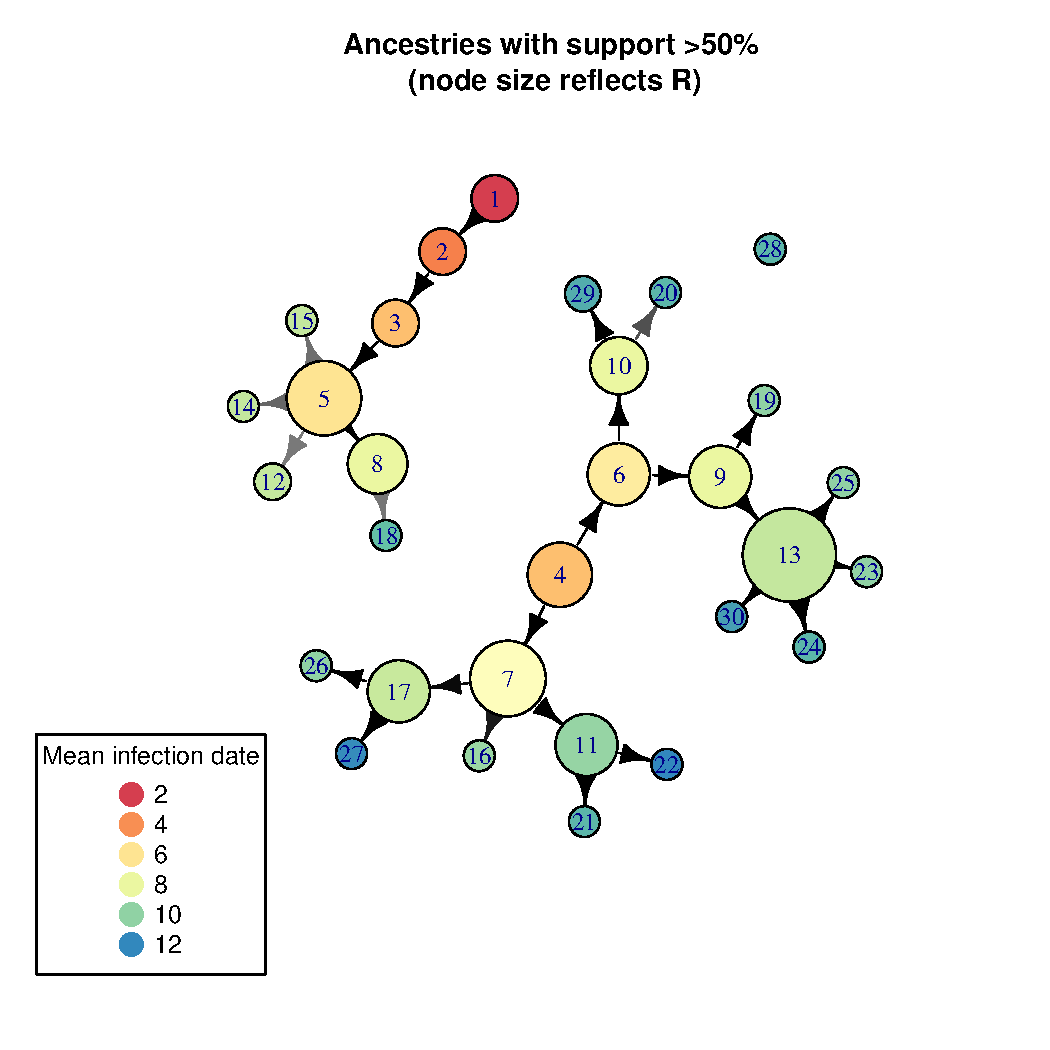
\includegraphics[width=.6\textwidth]{figs/unnamed-chunk-22} 

}



\end{knitrout}





\begin{knitrout}
\definecolor{shadecolor}{rgb}{0.969, 0.969, 0.969}\color{fgcolor}\begin{kframe}
\begin{alltt}
\hlkwd{plot}\hlstd{(}\hlkwd{get.tTree}\hlstd{(res),} \hlkwc{main}\hlstd{=}\hlstr{"Consensus ancestries - basic plot"}\hlstd{)}
\end{alltt}
\end{kframe}

{\centering 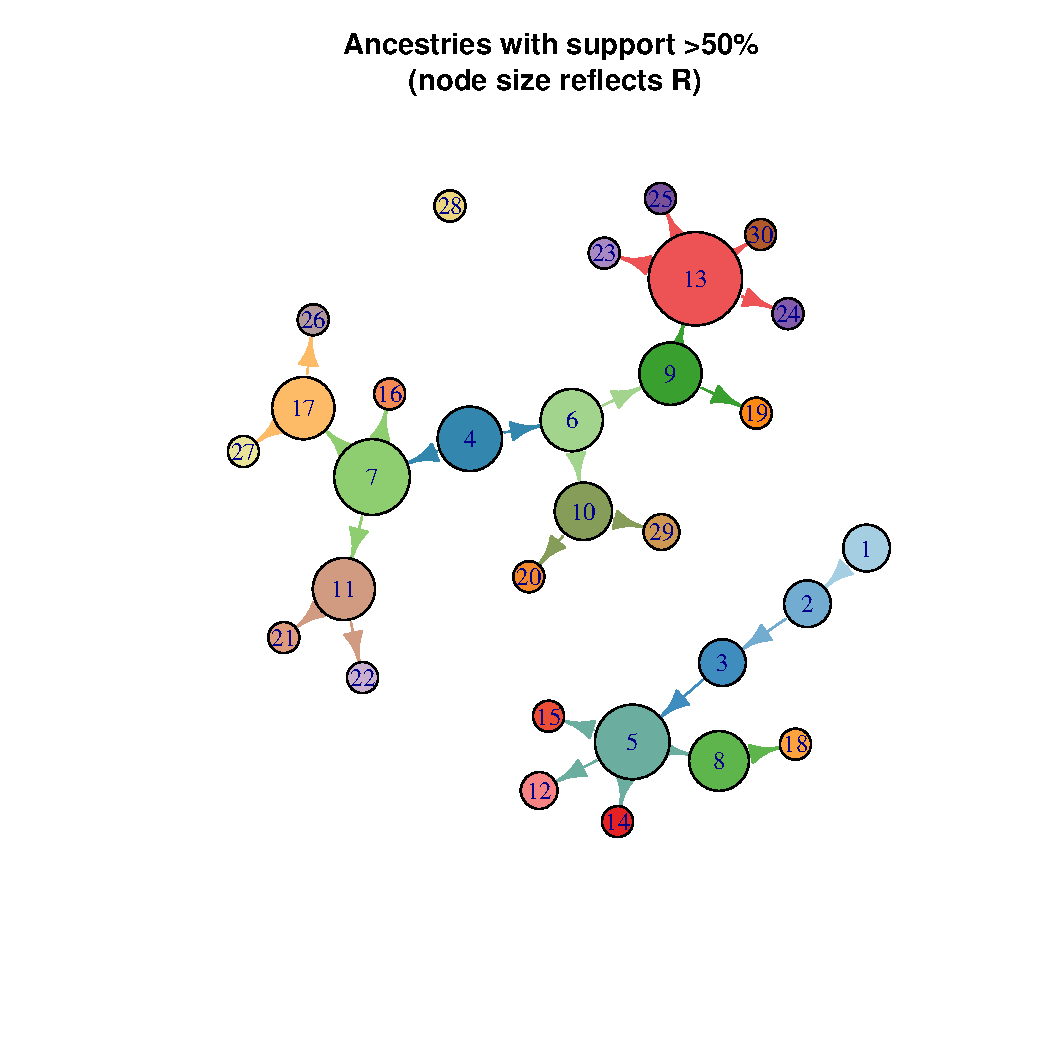
\includegraphics[width=.6\textwidth]{figs/unnamed-chunk-23} 

}



\end{knitrout}


\begin{knitrout}
\definecolor{shadecolor}{rgb}{0.969, 0.969, 0.969}\color{fgcolor}\begin{kframe}
\begin{alltt}
\hlstd{tre} \hlkwb{<-} \hlkwd{get.tTree}\hlstd{(res)}
\hlkwd{plot}\hlstd{(tre,} \hlkwc{edge.curved}\hlstd{=}\hlnum{TRUE}\hlstd{,} \hlkwc{vertex.color}\hlstd{=case.color}\hlopt{$}\hlstd{col,}
     \hlkwc{vertex.size}\hlstd{=case.size)}
\hlkwd{title}\hlstd{(}\hlstr{"Consensus ancestries \textbackslash{}n(x-axis represents time)"}\hlstd{)}
\hlkwd{legend}\hlstd{(}\hlstr{"bottomleft"}\hlstd{,} \hlkwc{col}\hlstd{=case.color}\hlopt{$}\hlstd{leg.col,} \hlkwc{leg}\hlstd{=case.color}\hlopt{$}\hlstd{leg.txt,} \hlkwc{title}\hlstd{=}\hlstr{"Mean infection date"}\hlstd{,} \hlkwc{pch}\hlstd{=}\hlnum{20}\hlstd{,} \hlkwc{pt.cex}\hlstd{=}\hlnum{3}\hlstd{,} \hlkwc{inset}\hlstd{=}\hlopt{-}\hlnum{.1}\hlstd{)}
\end{alltt}
\end{kframe}

{\centering 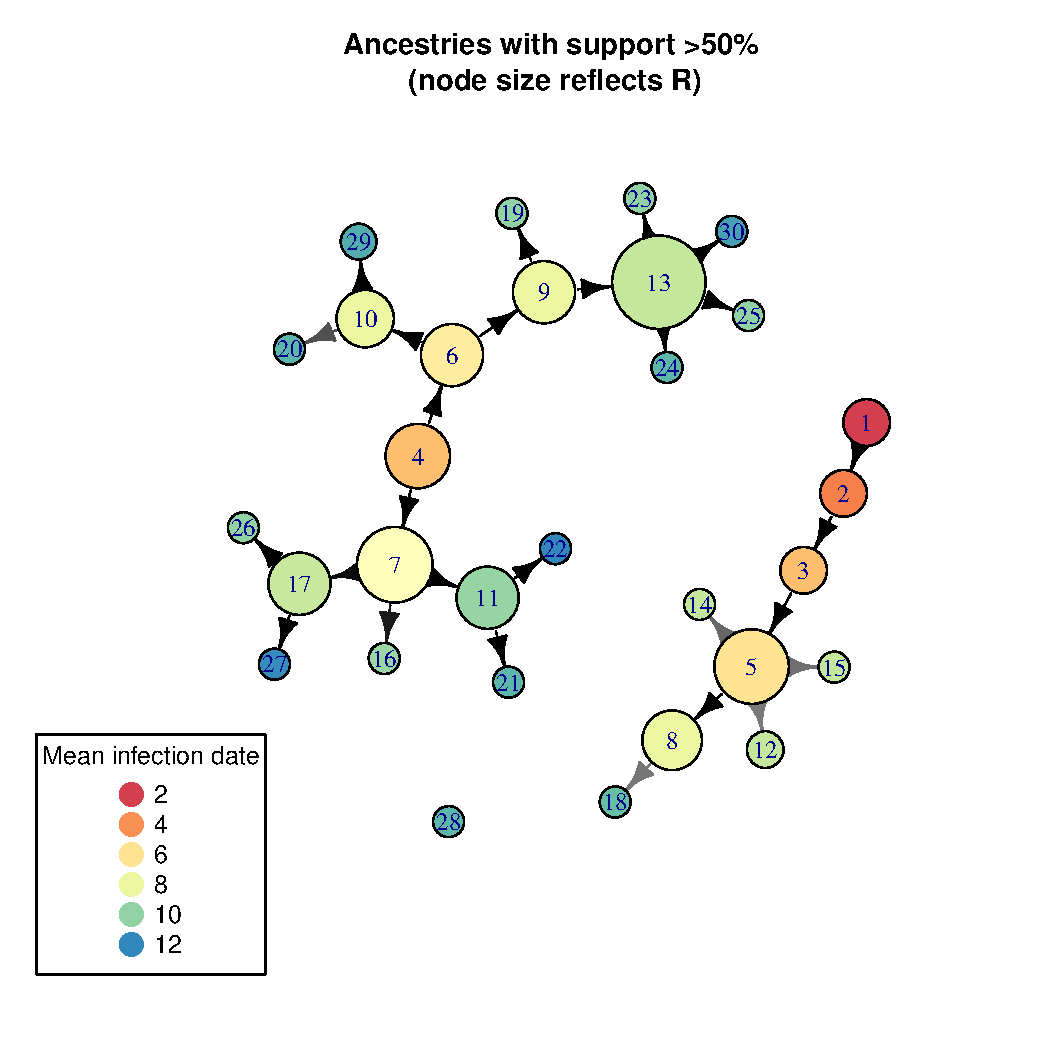
\includegraphics[width=.6\textwidth]{figs/unnamed-chunk-24} 

}



\end{knitrout}


\begin{knitrout}
\definecolor{shadecolor}{rgb}{0.969, 0.969, 0.969}\color{fgcolor}\begin{kframe}
\begin{alltt}
\hlstd{g} \hlkwb{<-} \hlkwd{as.igraph}\hlstd{(}\hlkwd{get.tTree}\hlstd{(res))}
\hlkwd{plot}\hlstd{(g,} \hlkwc{edge.curved}\hlstd{=}\hlnum{FALSE}\hlstd{,} \hlkwc{vertex.color}\hlstd{=case.color}\hlopt{$}\hlstd{col,} \hlkwc{layout}\hlstd{=layout.auto,} \hlkwc{vertex.size}\hlstd{=case.size,} \hlkwc{edge.label}\hlstd{=}\hlstr{""}\hlstd{)}
\hlkwd{title}\hlstd{(}\hlstr{"Consensus ancestries \textbackslash{}n(x-axis represents time)"}\hlstd{)}
\hlkwd{legend}\hlstd{(}\hlstr{"bottomleft"}\hlstd{,} \hlkwc{col}\hlstd{=case.color}\hlopt{$}\hlstd{leg.col,} \hlkwc{leg}\hlstd{=case.color}\hlopt{$}\hlstd{leg.txt,} \hlkwc{title}\hlstd{=}\hlstr{"Mean infection date"}\hlstd{,} \hlkwc{pch}\hlstd{=}\hlnum{20}\hlstd{,} \hlkwc{pt.cex}\hlstd{=}\hlnum{3}\hlstd{,} \hlkwc{inset}\hlstd{=}\hlopt{-}\hlnum{.1}\hlstd{)}
\end{alltt}
\end{kframe}

{\centering 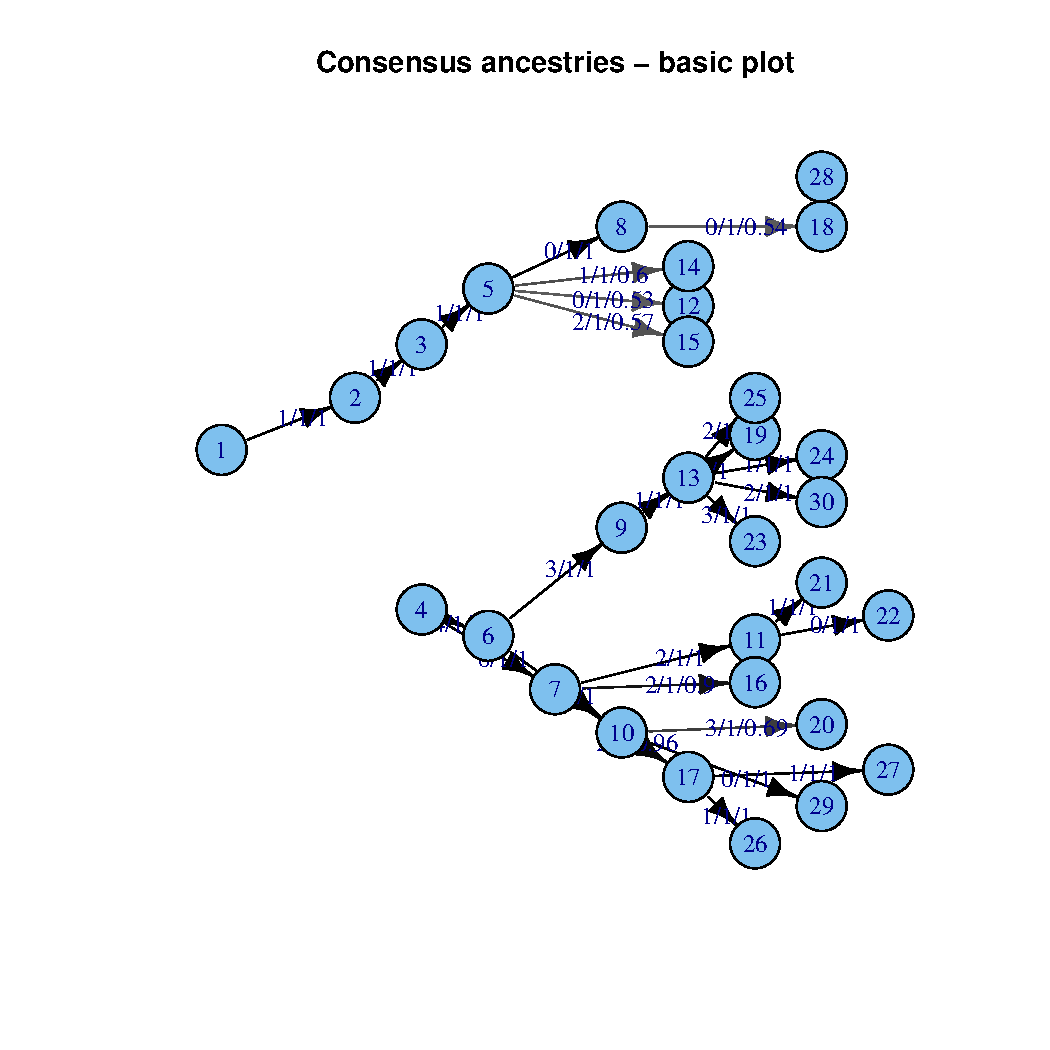
\includegraphics[width=.6\textwidth]{figs/unnamed-chunk-25} 

}



\end{knitrout}





%%%%%%%%%%%%%%%%%%%%%%%%%%%%%%%%%%%%%%%%%%%%%%%%%%%%
\subsection{Plotting dates of infection}
%%%%%%%%%%%%%%%%%%%%%%%%%%%%%%%%%%%%%%%%%%%%%%%%%%%%

\begin{knitrout}
\definecolor{shadecolor}{rgb}{0.969, 0.969, 0.969}\color{fgcolor}\begin{kframe}
\begin{alltt}
\hlstd{Tinf} \hlkwb{<-} \hlstd{x[x}\hlopt{$}\hlstd{step}\hlopt{>=}\hlnum{2e4}\hlstd{,}\hlkwd{c}\hlstd{(}\hlnum{1}\hlstd{,}\hlkwd{ncol}\hlstd{(x),}\hlkwd{grep}\hlstd{(}\hlstr{"Tinf"}\hlstd{,} \hlkwd{names}\hlstd{(x)))]}
\hlstd{Tinf[}\hlnum{1}\hlopt{:}\hlnum{5}\hlstd{,}\hlnum{1}\hlopt{:}\hlnum{6}\hlstd{]}
\end{alltt}
\begin{verbatim}
##     step run Tinf_1 Tinf_2 Tinf_3 Tinf_4
## 41 20000   1      2      4      5      5
## 42 20500   1      2      4      5      5
## 43 21000   1      2      4      5      5
## 44 21500   1      2      4      5      5
## 45 22000   1      2      3      5      5
\end{verbatim}
\end{kframe}
\end{knitrout}


\begin{knitrout}
\definecolor{shadecolor}{rgb}{0.969, 0.969, 0.969}\color{fgcolor}\begin{kframe}
\begin{alltt}
\hlstd{Tinf} \hlkwb{<-} \hlkwd{melt}\hlstd{(Tinf,} \hlkwc{id}\hlstd{=}\hlnum{1}\hlopt{:}\hlnum{2}\hlstd{)}
\hlkwd{names}\hlstd{(Tinf)[}\hlnum{3}\hlopt{:}\hlnum{4}\hlstd{]} \hlkwb{<-} \hlkwd{c}\hlstd{(}\hlstr{"case"}\hlstd{,} \hlstr{"date"}\hlstd{)}
\hlstd{Tinf}\hlopt{$}\hlstd{case} \hlkwb{<-} \hlkwd{sub}\hlstd{(}\hlstr{"Tinf_"}\hlstd{,}\hlstr{"Case "}\hlstd{, Tinf}\hlopt{$}\hlstd{case)}
\hlstd{Tinf}\hlopt{$}\hlstd{case} \hlkwb{<-} \hlkwd{factor}\hlstd{(Tinf}\hlopt{$}\hlstd{case,} \hlkwc{levels}\hlstd{=}\hlkwd{paste}\hlstd{(}\hlstr{"Case"}\hlstd{,}\hlnum{1}\hlopt{:}\hlnum{30}\hlstd{))}
\hlkwd{head}\hlstd{(Tinf)}
\end{alltt}
\begin{verbatim}
##    step run   case date
## 1 20000   1 Case 1    2
## 2 20500   1 Case 1    2
## 3 21000   1 Case 1    2
## 4 21500   1 Case 1    2
## 5 22000   1 Case 1    2
## 6 22500   1 Case 1    2
\end{verbatim}
\begin{alltt}
\hlkwd{tail}\hlstd{(Tinf)}
\end{alltt}
\begin{verbatim}
##         step run    case date
## 19315  97500   4 Case 30   11
## 19316  98000   4 Case 30   12
## 19317  98500   4 Case 30   12
## 19318  99000   4 Case 30   12
## 19319  99500   4 Case 30   12
## 19320 100000   4 Case 30   11
\end{verbatim}
\end{kframe}
\end{knitrout}


\begin{knitrout}
\definecolor{shadecolor}{rgb}{0.969, 0.969, 0.969}\color{fgcolor}\begin{kframe}
\begin{alltt}
\hlkwd{ggplot}\hlstd{(}\hlkwc{data}\hlstd{=Tinf)} \hlopt{+} \hlkwd{geom_line}\hlstd{(}\hlkwd{aes}\hlstd{(}\hlkwc{x}\hlstd{=step,}\hlkwc{y}\hlstd{=date,}\hlkwc{colour}\hlstd{=case),} \hlkwc{alpha}\hlstd{=}\hlnum{.5}\hlstd{)} \hlopt{+}
    \hlkwd{labs}\hlstd{(}\hlkwc{y}\hlstd{=}\hlstr{"Infection date"}\hlstd{,} \hlkwc{title}\hlstd{=}\hlstr{"Traces of infection dates"}\hlstd{)}
\end{alltt}
\end{kframe}

{\centering 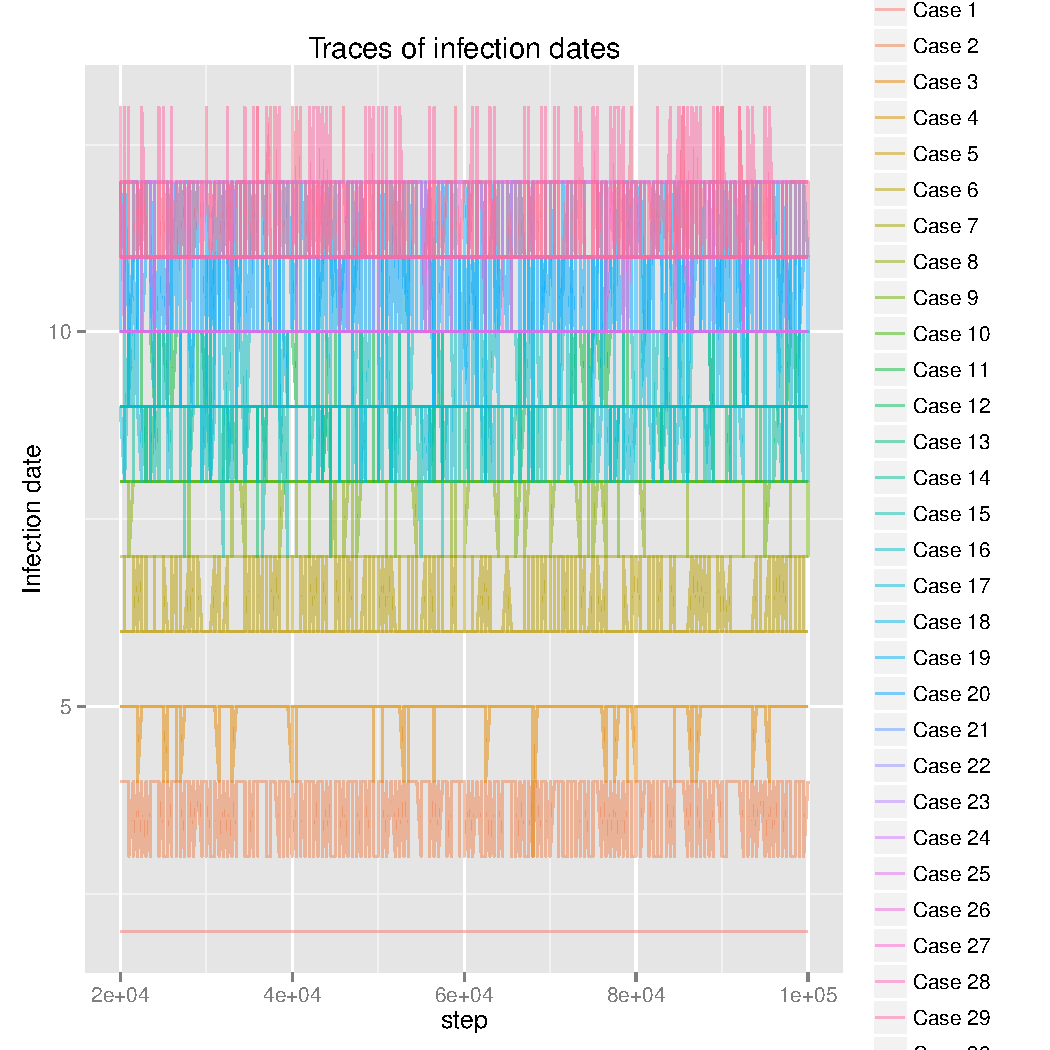
\includegraphics[width=.6\textwidth]{figs/unnamed-chunk-28} 

}



\end{knitrout}



\begin{knitrout}
\definecolor{shadecolor}{rgb}{0.969, 0.969, 0.969}\color{fgcolor}\begin{kframe}
\begin{alltt}
\hlkwd{ggplot}\hlstd{(}\hlkwc{data}\hlstd{=Tinf)} \hlopt{+} \hlkwd{geom_boxplot}\hlstd{(}\hlkwd{aes}\hlstd{(}\hlkwc{x}\hlstd{=case,}\hlkwc{y}\hlstd{=date,}\hlkwc{fill}\hlstd{=case,} \hlkwc{alpha}\hlstd{=}\hlnum{.5}\hlstd{))} \hlopt{+}
   \hlkwd{coord_flip}\hlstd{()} \hlopt{+} \hlkwd{labs}\hlstd{(}\hlkwc{y}\hlstd{=}\hlstr{"Infection date"}\hlstd{,} \hlkwc{x}\hlstd{=}\hlstr{""}\hlstd{,} \hlkwc{title}\hlstd{=}\hlstr{"Distribution of infection dates"}\hlstd{)}
\end{alltt}
\end{kframe}

{\centering 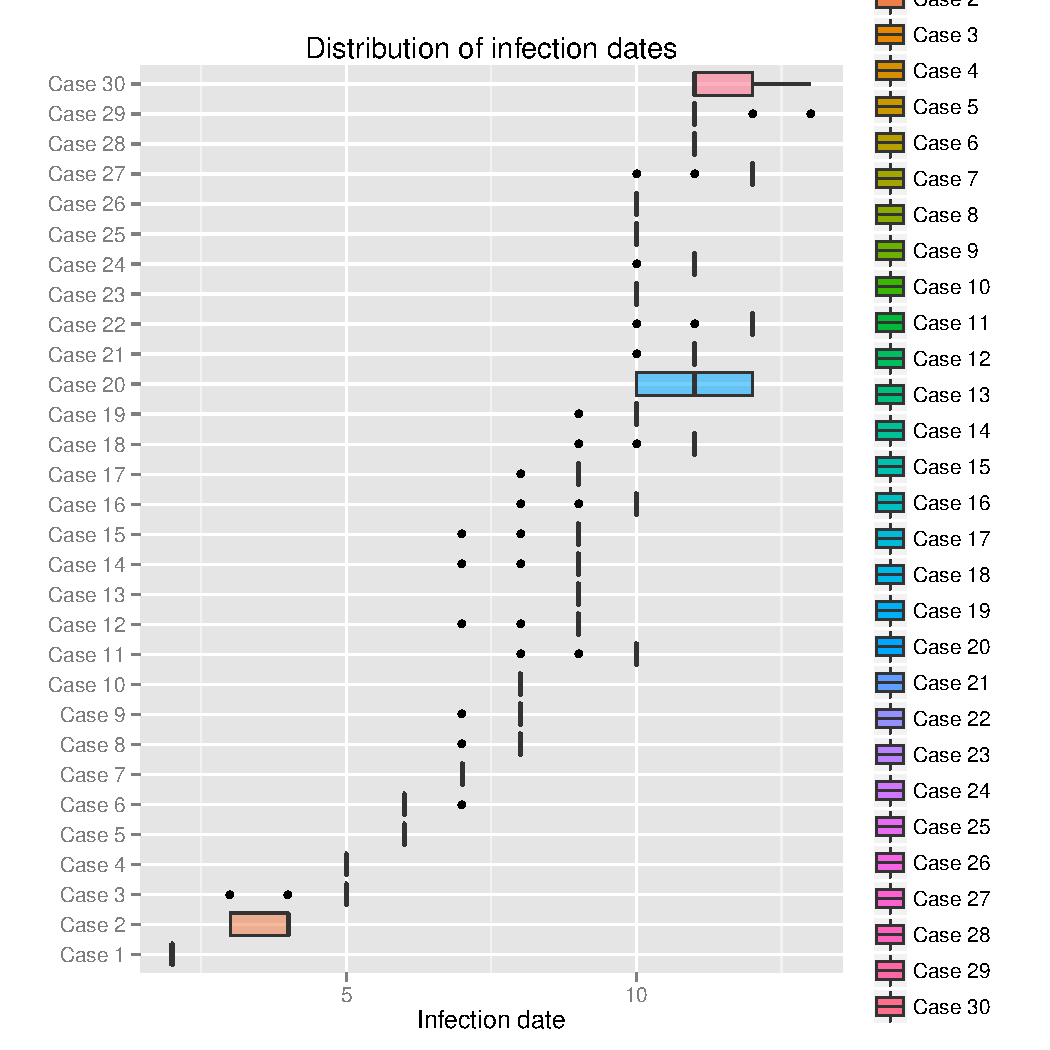
\includegraphics[width=.6\textwidth]{figs/unnamed-chunk-29} 

}



\end{knitrout}



\begin{knitrout}
\definecolor{shadecolor}{rgb}{0.969, 0.969, 0.969}\color{fgcolor}\begin{kframe}
\begin{alltt}
\hlkwd{ggplot}\hlstd{(}\hlkwc{data}\hlstd{=Tinf)} \hlopt{+} \hlkwd{geom_boxplot}\hlstd{(}\hlkwd{aes}\hlstd{(}\hlkwc{x}\hlstd{=case,}\hlkwc{y}\hlstd{=date,}\hlkwc{fill}\hlstd{=run),}\hlkwc{alpha}\hlstd{=}\hlnum{.5}\hlstd{)} \hlopt{+} \hlkwd{coord_flip}\hlstd{()} \hlopt{+}
    \hlkwd{labs}\hlstd{(}\hlkwc{y}\hlstd{=}\hlstr{"Infection date"}\hlstd{,} \hlkwc{x}\hlstd{=}\hlstr{""}\hlstd{,} \hlkwc{title}\hlstd{=}\hlstr{"Distribution of infection dates"}\hlstd{)}
\end{alltt}
\end{kframe}

{\centering 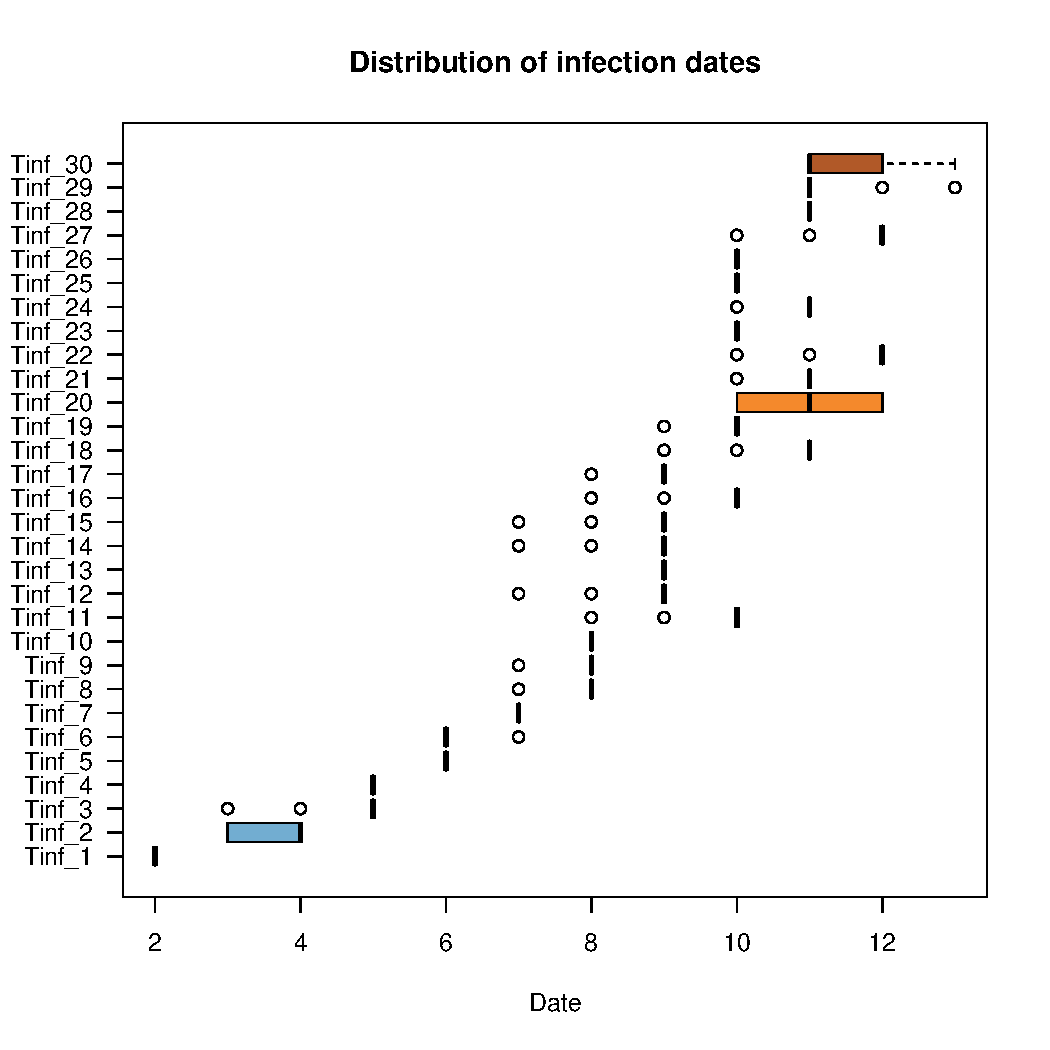
\includegraphics[width=.6\textwidth]{figs/unnamed-chunk-30} 

}



\end{knitrout}





%%%%%%%%%%%%%%%%%%%%%%%%%%%%%%%%%%%%%%%%%%%%%%%%%%%%
\subsection{Accessing posterior distributions}
%%%%%%%%%%%%%%%%%%%%%%%%%%%%%%%%%%%%%%%%%%%%%%%%%%%%


Note that any element of the model in \texttt{res\$chains} can be plotted using \texttt{plotChains};
for instance, the mutation rate:
\begin{knitrout}
\definecolor{shadecolor}{rgb}{0.969, 0.969, 0.969}\color{fgcolor}\begin{kframe}
\begin{alltt}
\hlkwd{plotChains}\hlstd{(res,} \hlkwc{main}\hlstd{=}\hlstr{"Trace of mu \textbackslash{}n(burnin removed)"}\hlstd{,}
           \hlkwc{burnin}\hlstd{=}\hlnum{2e4}\hlstd{,} \hlkwc{what}\hlstd{=}\hlstr{"mu1"}\hlstd{)}
\end{alltt}
\end{kframe}

{\centering 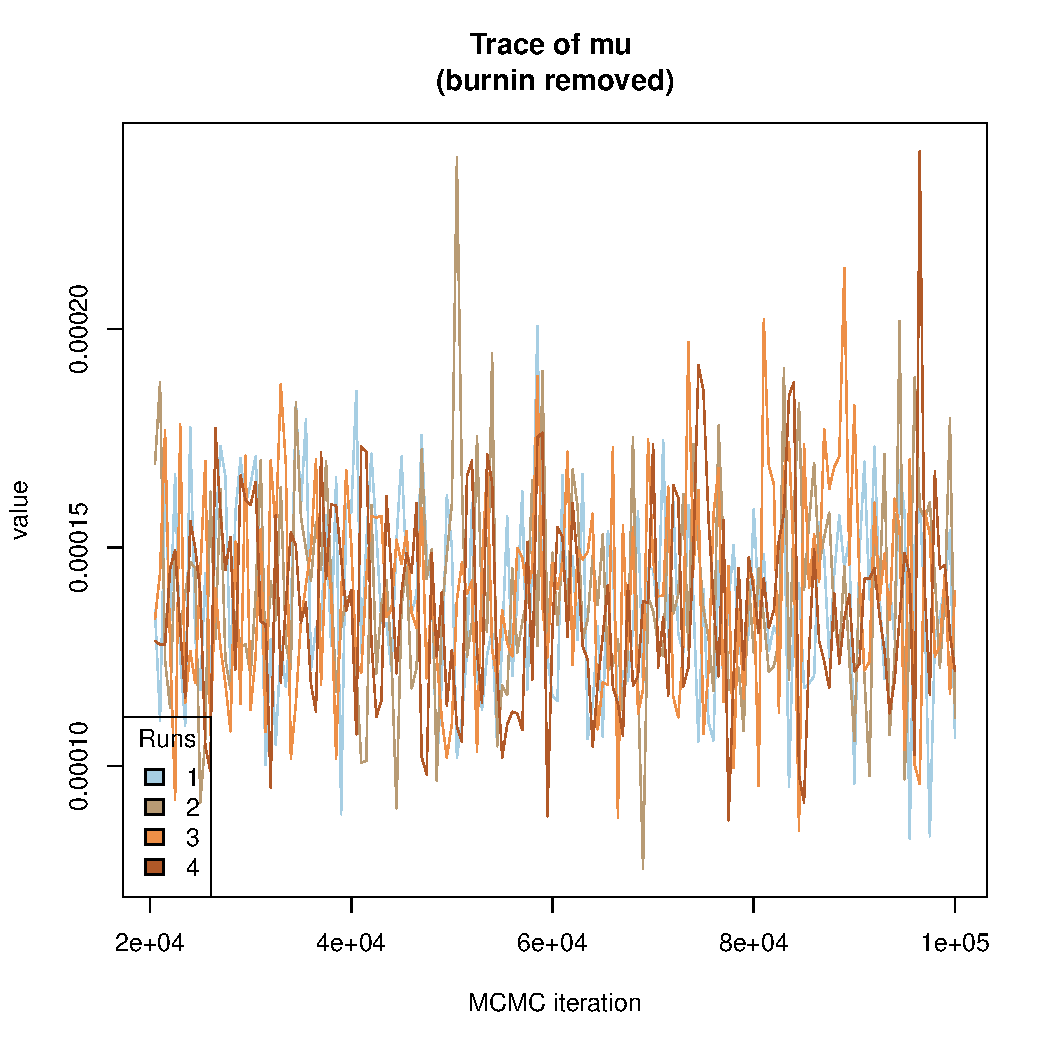
\includegraphics[width=.6\textwidth]{figs/unnamed-chunk-311} 

}


\begin{kframe}\begin{alltt}
\hlkwd{plotChains}\hlstd{(res,} \hlkwc{main}\hlstd{=}\hlstr{"Trace of mu \textbackslash{}n(burnin removed)"}\hlstd{,}
           \hlkwc{burnin}\hlstd{=}\hlnum{2e4}\hlstd{,} \hlkwc{what}\hlstd{=}\hlstr{"mu1"}\hlstd{,} \hlkwc{type}\hlstd{=}\hlstr{"dens"}\hlstd{)}
\end{alltt}
\end{kframe}

{\centering 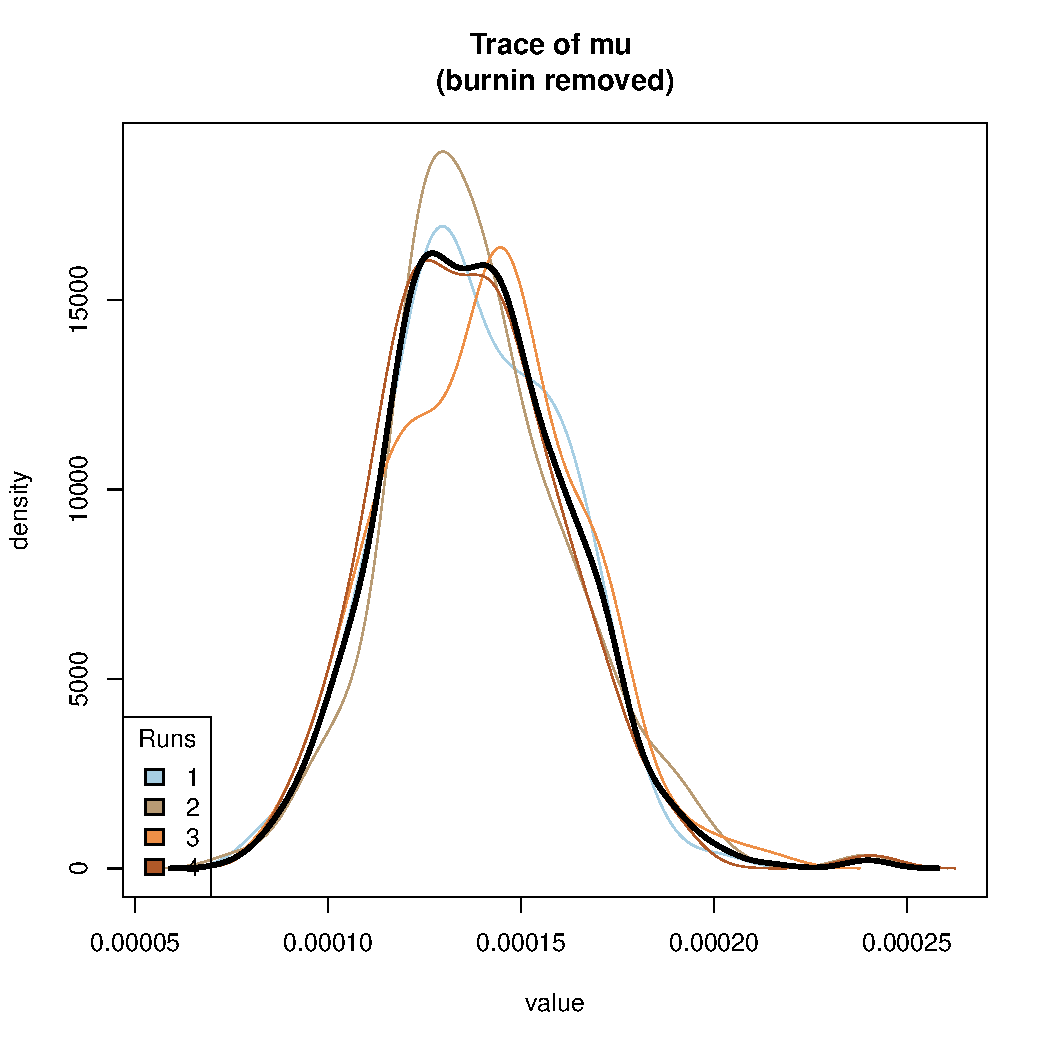
\includegraphics[width=.6\textwidth]{figs/unnamed-chunk-312} 

}



\end{knitrout}

(note that in this case, the plotted information is the mutation rate \textit{per generation of
  infection}, and not per unit of time.
See section on mutation rates below for an estimation of the rates per unit of time.



\begin{knitrout}
\definecolor{shadecolor}{rgb}{0.969, 0.969, 0.969}\color{fgcolor}\begin{kframe}
\begin{alltt}
\hlkwd{library}\hlstd{(ggplot2)}
\hlkwd{library}\hlstd{(reshape2)}
\hlstd{x} \hlkwb{<-} \hlstd{res}\hlopt{$}\hlstd{chains[x}\hlopt{$}\hlstd{step}\hlopt{>}\hlnum{2e4}\hlstd{,]}
\hlstd{x}\hlopt{$}\hlstd{run} \hlkwb{<-} \hlkwd{factor}\hlstd{(x}\hlopt{$}\hlstd{run)}
\end{alltt}
\end{kframe}
\end{knitrout}


\begin{knitrout}
\definecolor{shadecolor}{rgb}{0.969, 0.969, 0.969}\color{fgcolor}\begin{kframe}
\begin{alltt}
\hlstd{p} \hlkwb{<-} \hlkwd{ggplot}\hlstd{(}\hlkwc{data}\hlstd{=x)} \hlopt{+} \hlkwd{labs}\hlstd{(}\hlkwc{title}\hlstd{=}\hlstr{"Posterior distribution of pi"}\hlstd{,} \hlkwc{x}\hlstd{=}\hlstr{"Pi (proportion of cases sampled)"}\hlstd{)}
\hlstd{p} \hlopt{+} \hlkwd{geom_density}\hlstd{(}\hlkwd{aes}\hlstd{(}\hlkwc{x}\hlstd{=pi,} \hlkwc{fill}\hlstd{=run),} \hlkwc{alpha}\hlstd{=}\hlnum{.3}\hlstd{,} \hlkwc{colour}\hlstd{=}\hlnum{NA}\hlstd{)} \hlopt{+}
    \hlkwd{geom_density}\hlstd{(}\hlkwd{aes}\hlstd{(}\hlkwc{x}\hlstd{=pi),} \hlkwc{size}\hlstd{=}\hlnum{1}\hlstd{,} \hlkwc{colour}\hlstd{=}\hlstr{"black"}\hlstd{,} \hlkwc{shape}\hlstd{=}\hlnum{2}\hlstd{,} \hlkwc{alpha}\hlstd{=}\hlnum{.8}\hlstd{)}
\end{alltt}
\end{kframe}

{\centering 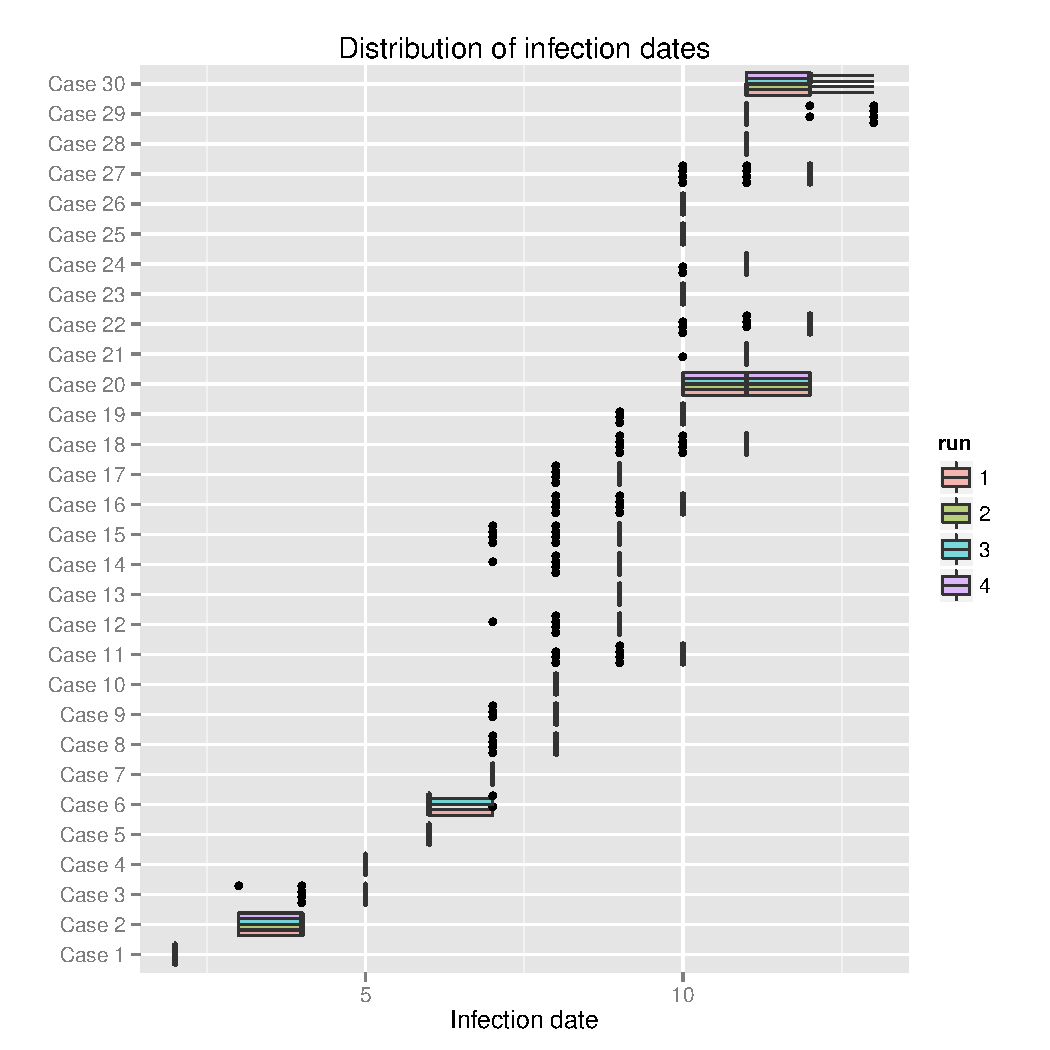
\includegraphics[width=.6\textwidth]{figs/unnamed-chunk-33} 

}



\end{knitrout}


\begin{knitrout}
\definecolor{shadecolor}{rgb}{0.969, 0.969, 0.969}\color{fgcolor}\begin{kframe}
\begin{alltt}
\hlstd{p} \hlopt{+} \hlkwd{geom_histogram}\hlstd{(}\hlkwd{aes}\hlstd{(}\hlkwc{x}\hlstd{=pi,} \hlkwc{fill}\hlstd{=run,} \hlkwc{y}\hlstd{=..density..),} \hlkwc{alpha}\hlstd{=}\hlnum{.7}\hlstd{,} \hlkwc{colour}\hlstd{=}\hlnum{NA}\hlstd{,} \hlkwc{position}\hlstd{=}\hlstr{"dodge"}\hlstd{)} \hlopt{+}
    \hlkwd{geom_density}\hlstd{(}\hlkwd{aes}\hlstd{(}\hlkwc{x}\hlstd{=pi),} \hlkwc{size}\hlstd{=}\hlnum{1}\hlstd{,} \hlkwc{colour}\hlstd{=}\hlstr{"black"}\hlstd{,} \hlkwc{shape}\hlstd{=}\hlnum{2}\hlstd{,} \hlkwc{alpha}\hlstd{=}\hlnum{.8}\hlstd{)}
\end{alltt}


{\ttfamily\noindent\itshape\color{messagecolor}{\#\# stat\_bin: binwidth defaulted to range/30. Use 'binwidth = x' to adjust this.}}\end{kframe}

{\centering 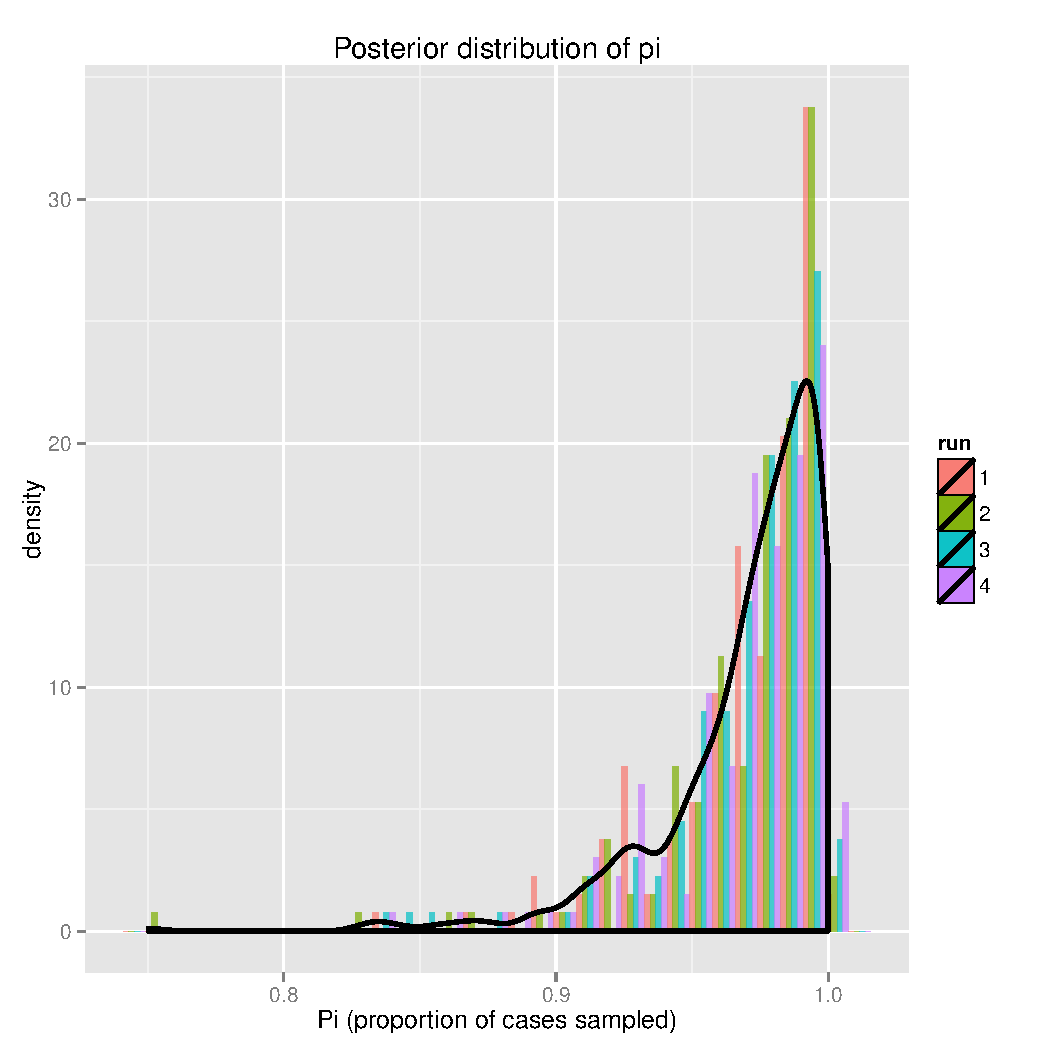
\includegraphics[width=.6\textwidth]{figs/unnamed-chunk-34} 

}



\end{knitrout}



\begin{knitrout}
\definecolor{shadecolor}{rgb}{0.969, 0.969, 0.969}\color{fgcolor}\begin{kframe}
\begin{alltt}
\hlstd{p} \hlopt{+} \hlkwd{geom_boxplot}\hlstd{(}\hlkwd{aes}\hlstd{(}\hlkwc{x}\hlstd{=run,} \hlkwc{y}\hlstd{=pi,} \hlkwc{fill}\hlstd{=run),}\hlkwc{alpha}\hlstd{=}\hlnum{.6}\hlstd{)} \hlopt{+} \hlkwd{geom_jitter}\hlstd{(}\hlkwd{aes}\hlstd{(}\hlkwc{x}\hlstd{=run,} \hlkwc{y}\hlstd{=pi,} \hlkwc{col}\hlstd{=run),}\hlkwc{alpha}\hlstd{=}\hlnum{.4}\hlstd{)}
\end{alltt}
\end{kframe}

{\centering 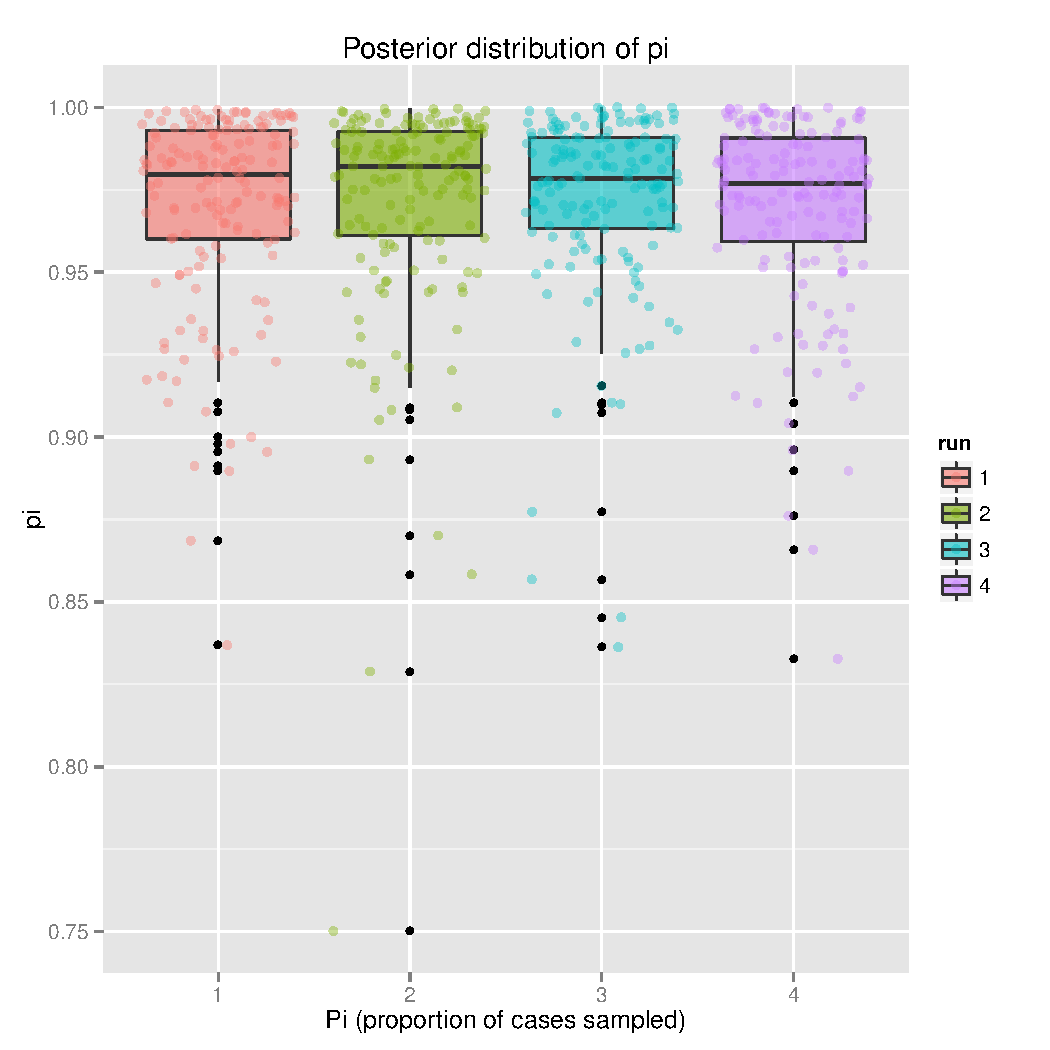
\includegraphics[width=.6\textwidth]{figs/unnamed-chunk-35} 

}



\end{knitrout}


\begin{knitrout}
\definecolor{shadecolor}{rgb}{0.969, 0.969, 0.969}\color{fgcolor}\begin{kframe}
\begin{alltt}
\hlstd{p} \hlopt{+} \hlkwd{geom_violin}\hlstd{(}\hlkwd{aes}\hlstd{(}\hlkwc{x}\hlstd{=run,} \hlkwc{y}\hlstd{=pi,} \hlkwc{fill}\hlstd{=run),}\hlkwc{alpha}\hlstd{=}\hlnum{.6}\hlstd{)}
\end{alltt}
\end{kframe}

{\centering 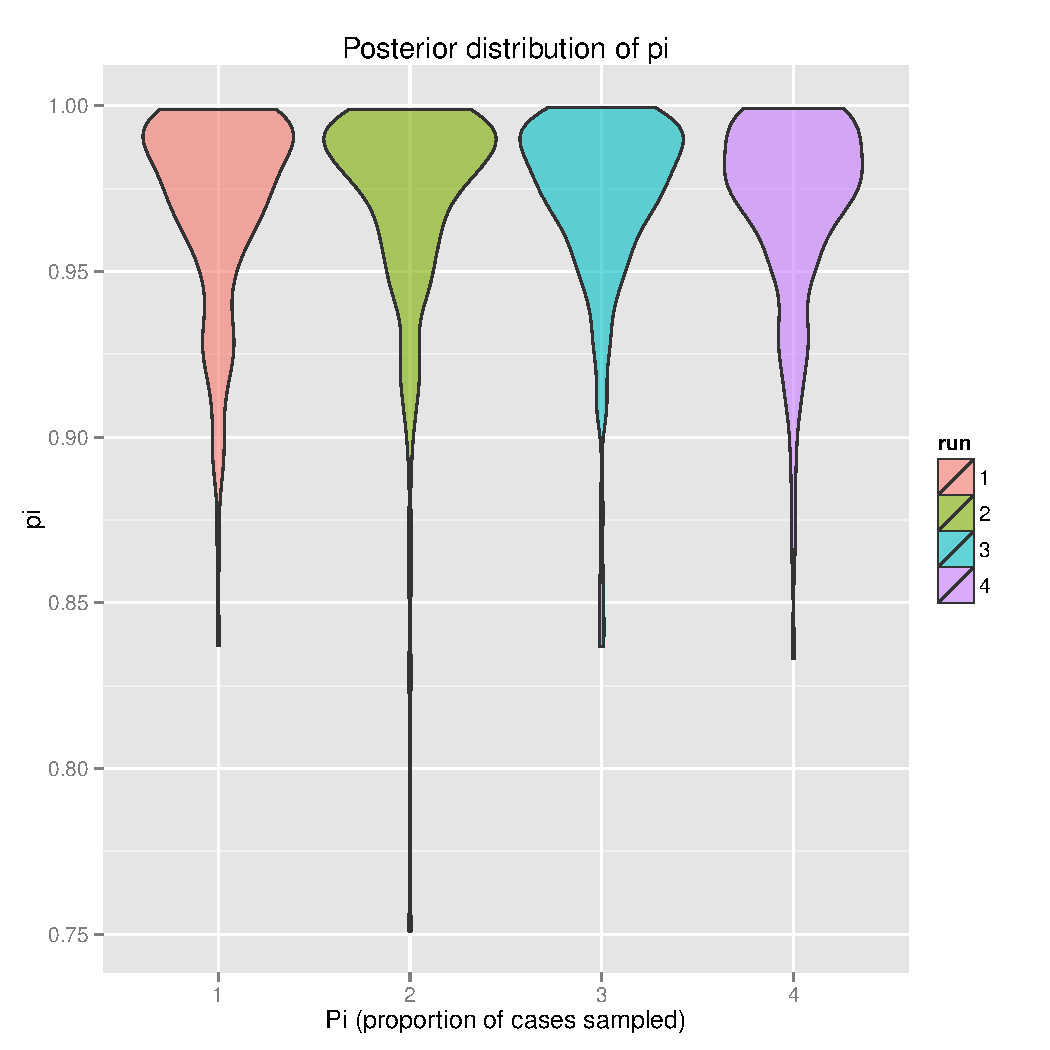
\includegraphics[width=.6\textwidth]{figs/unnamed-chunk-36} 

}



\end{knitrout}






%%%%%%%%%%%%%%%%%%%%%%%%%%%%%%%%%%%%%%%%%%%%%%%%%%%%
\subsection{Mutation rates}
%%%%%%%%%%%%%%%%%%%%%%%%%%%%%%%%%%%%%%%%%%%%%%%%%%%%

\begin{knitrout}
\definecolor{shadecolor}{rgb}{0.969, 0.969, 0.969}\color{fgcolor}\begin{kframe}
\begin{alltt}
\hlstd{mu} \hlkwb{<-} \hlkwd{get.mu}\hlstd{(res,} \hlkwc{burnin}\hlstd{=}\hlnum{2e4}\hlstd{)}
\hlkwd{hist}\hlstd{(mu,} \hlkwc{col}\hlstd{=}\hlstr{"grey"}\hlstd{,}\hlkwc{border}\hlstd{=}\hlstr{"lightgrey"}\hlstd{,} \hlkwc{xlab}\hlstd{=}\hlstr{"Mutation rate (per genome and unit time)"}\hlstd{,}
     \hlkwc{main}\hlstd{=}\hlstr{"Posterior distribution of mu"}\hlstd{)}
\end{alltt}
\end{kframe}

{\centering 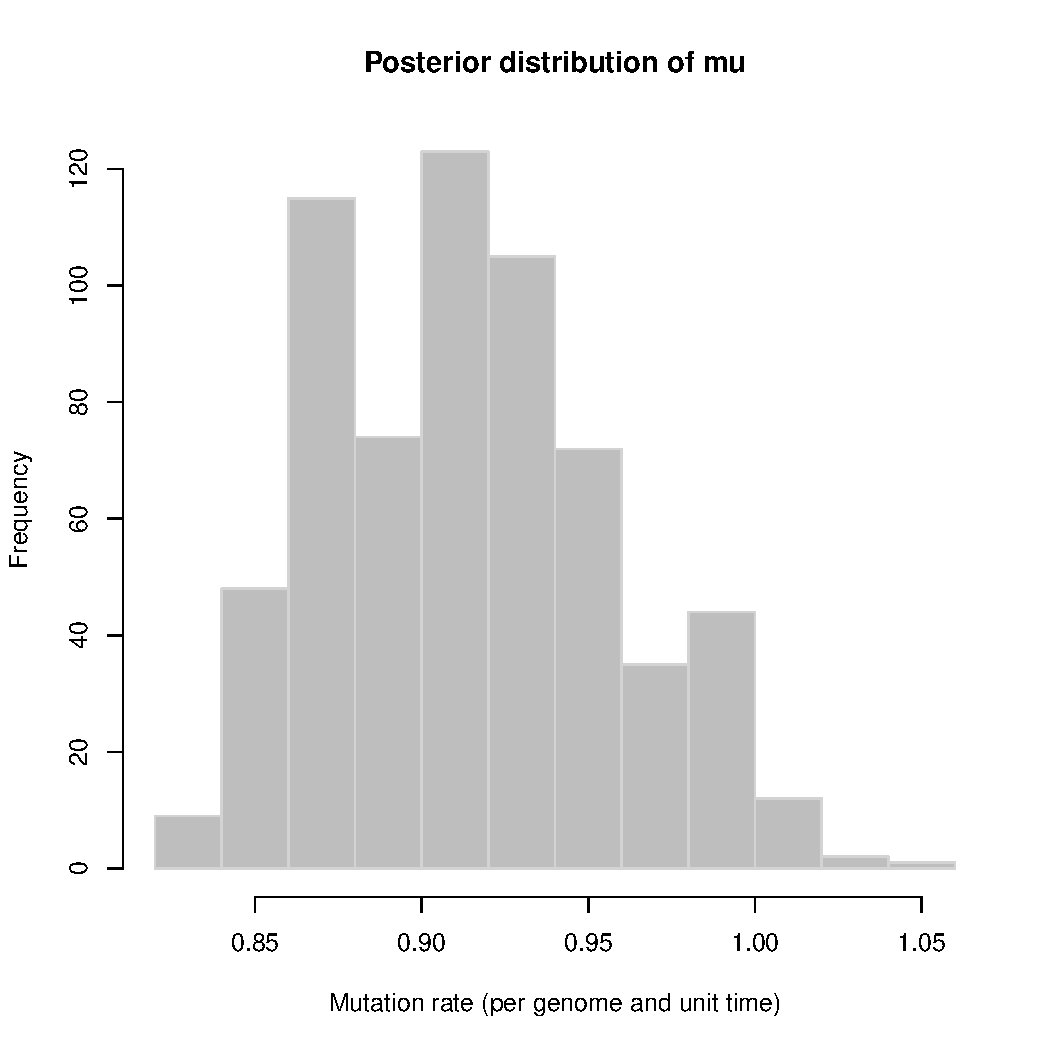
\includegraphics[width=.6\textwidth]{figs/unnamed-chunk-37} 

}



\end{knitrout}



\begin{knitrout}
\definecolor{shadecolor}{rgb}{0.969, 0.969, 0.969}\color{fgcolor}\begin{kframe}
\begin{alltt}
\hlstd{mu} \hlkwb{<-} \hlkwd{get.mu}\hlstd{(res,} \hlkwc{burnin}\hlstd{=}\hlnum{2e4}\hlstd{,} \hlkwc{genome.size}\hlstd{=}\hlkwd{ncol}\hlstd{(dat}\hlopt{$}\hlstd{dna))}
\hlkwd{summary}\hlstd{(mu)}
\end{alltt}
\begin{verbatim}
##     Min.  1st Qu.   Median     Mean  3rd Qu.     Max. 
## 8.27e-05 8.77e-05 9.14e-05 9.14e-05 9.44e-05 1.06e-04
\end{verbatim}
\begin{alltt}
\hlkwd{hist}\hlstd{(mu,} \hlkwc{col}\hlstd{=}\hlstr{"grey"}\hlstd{,}\hlkwc{border}\hlstd{=}\hlstr{"lightgrey"}\hlstd{,} \hlkwc{xlab}\hlstd{=}\hlstr{"Mutation rate (per genome and unit time)"}\hlstd{,}
     \hlkwc{main}\hlstd{=}\hlstr{"Posterior distribution of mu"}\hlstd{)}
\hlkwd{abline}\hlstd{(}\hlkwc{v}\hlstd{=}\hlkwd{quantile}\hlstd{(mu,} \hlkwd{c}\hlstd{(}\hlnum{.025}\hlstd{,} \hlnum{.5}\hlstd{,} \hlnum{.975}\hlstd{)),} \hlkwc{lty}\hlstd{=}\hlkwd{c}\hlstd{(}\hlnum{2}\hlstd{,}\hlnum{1}\hlstd{,}\hlnum{2}\hlstd{),} \hlkwc{lwd}\hlstd{=}\hlnum{2}\hlstd{,} \hlkwc{col}\hlstd{=}\hlstr{"royalblue"}\hlstd{)}
\end{alltt}
\end{kframe}

{\centering 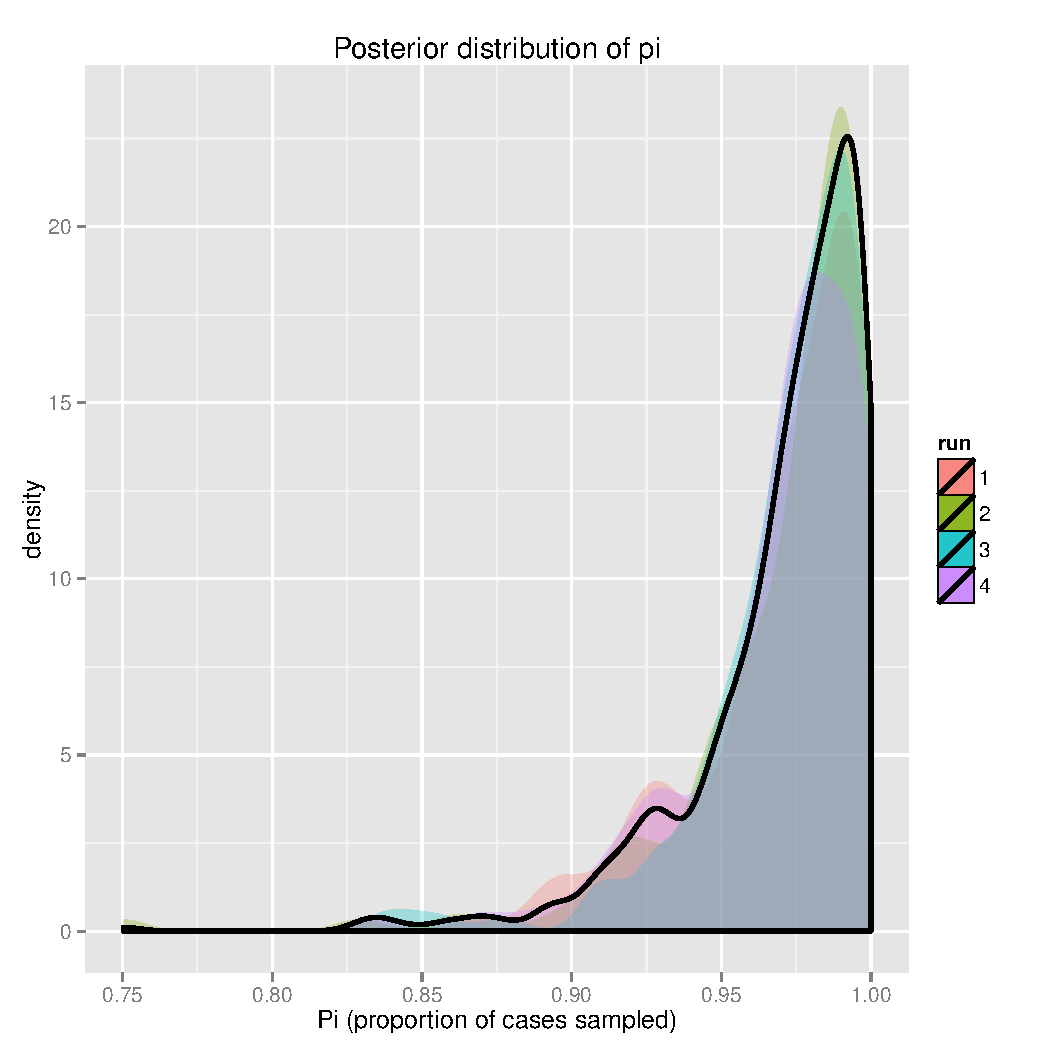
\includegraphics[width=.6\textwidth]{figs/unnamed-chunk-38} 

}



\end{knitrout}



\begin{knitrout}
\definecolor{shadecolor}{rgb}{0.969, 0.969, 0.969}\color{fgcolor}\begin{kframe}
\begin{alltt}
\hlkwd{plot}\hlstd{(}\hlkwd{density}\hlstd{(mu),} \hlkwc{xlab}\hlstd{=}\hlstr{"Mutation rate (per genome and unit time)"}\hlstd{,}
     \hlkwc{main}\hlstd{=}\hlstr{"Posterior distribution of mu"}\hlstd{,} \hlkwc{lwd}\hlstd{=}\hlnum{3}\hlstd{)}
\hlkwd{points}\hlstd{(}\hlkwd{jitter}\hlstd{(mu),} \hlkwd{rep}\hlstd{(}\hlnum{0}\hlstd{,} \hlkwd{length}\hlstd{(mu)),} \hlkwc{pch}\hlstd{=}\hlstr{"|"}\hlstd{,} \hlkwc{col}\hlstd{=}\hlkwd{transp}\hlstd{(}\hlstr{"blue"}\hlstd{))}
\hlkwd{abline}\hlstd{(}\hlkwc{v}\hlstd{=}\hlkwd{quantile}\hlstd{(mu,} \hlkwd{c}\hlstd{(}\hlnum{.025}\hlstd{,} \hlnum{.5}\hlstd{,} \hlnum{.975}\hlstd{)),} \hlkwc{lty}\hlstd{=}\hlkwd{c}\hlstd{(}\hlnum{2}\hlstd{,}\hlnum{1}\hlstd{,}\hlnum{2}\hlstd{),} \hlkwc{lwd}\hlstd{=}\hlnum{2}\hlstd{,} \hlkwc{col}\hlstd{=}\hlstr{"royalblue"}\hlstd{)}
\end{alltt}
\end{kframe}

{\centering 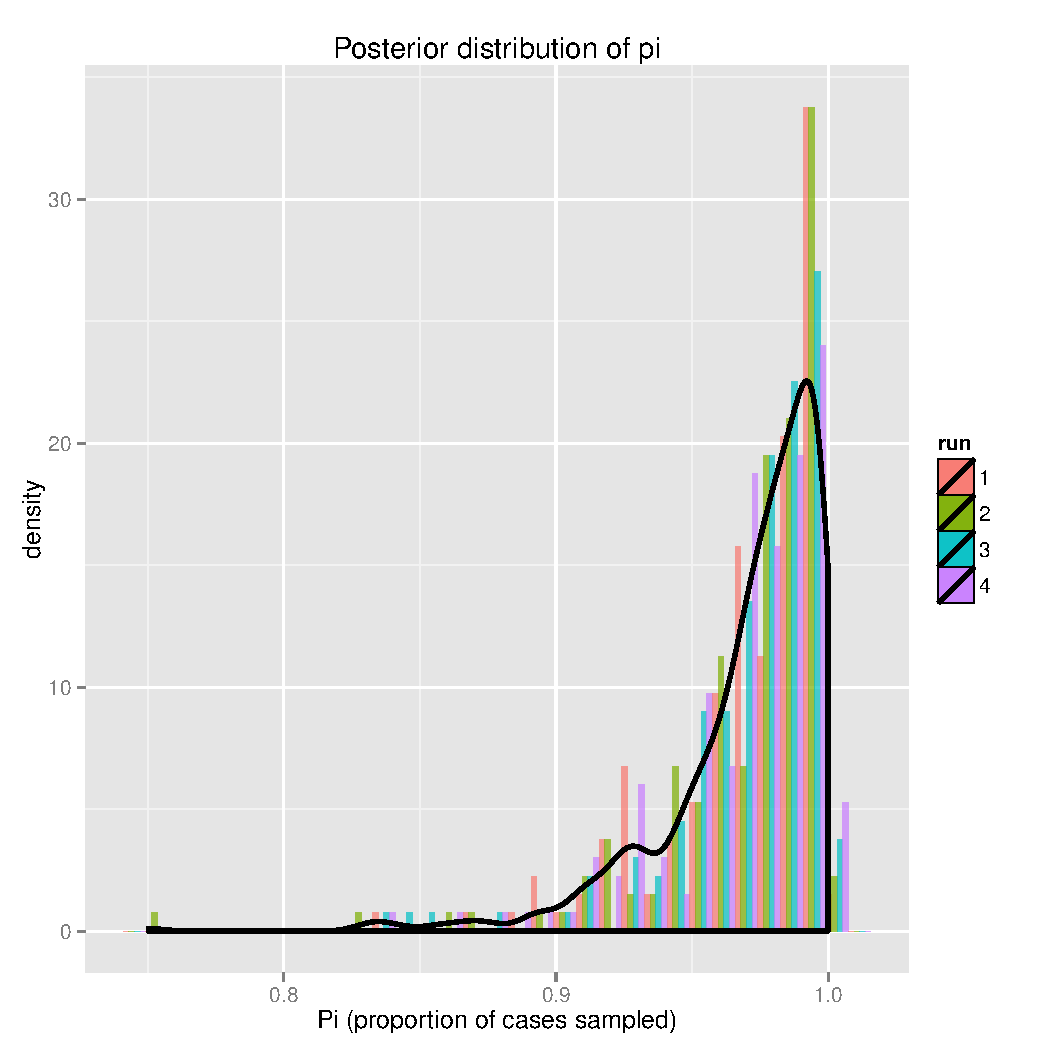
\includegraphics[width=.6\textwidth]{figs/unnamed-chunk-39} 

}



\end{knitrout}






%%%%%%%%%%%%%%%%%%%%%%%%%%%%%%%%%%%%%%%%%%%%%%%%%%%%
\subsection{Incidence and reproduction numbers}
%%%%%%%%%%%%%%%%%%%%%%%%%%%%%%%%%%%%%%%%%%%%%%%%%%%%

\begin{knitrout}
\definecolor{shadecolor}{rgb}{0.969, 0.969, 0.969}\color{fgcolor}\begin{kframe}
\begin{alltt}
\hlstd{incid} \hlkwb{<-} \hlkwd{get.incid}\hlstd{(res)}
\end{alltt}
\end{kframe}

{\centering 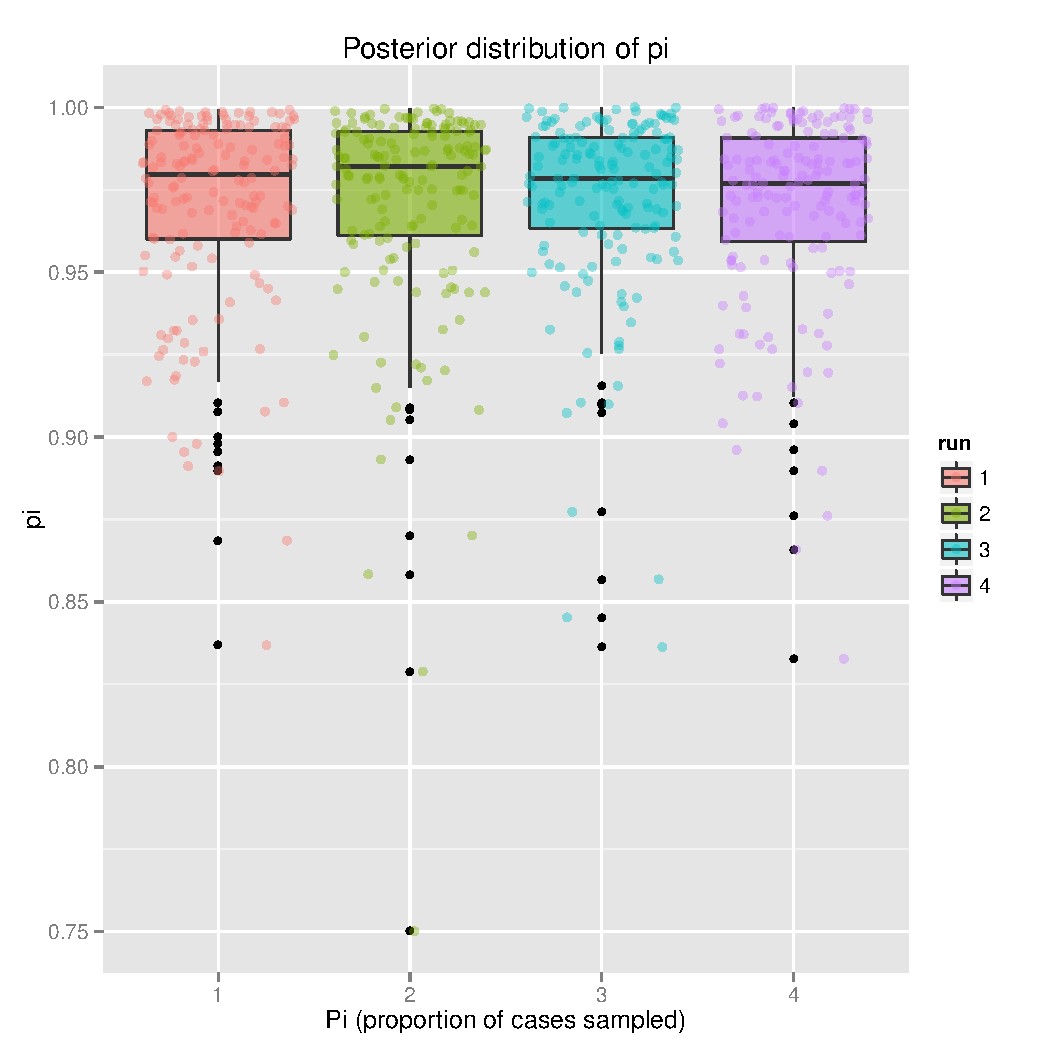
\includegraphics[width=.6\textwidth]{figs/unnamed-chunk-40} 

}



\end{knitrout}


\begin{knitrout}
\definecolor{shadecolor}{rgb}{0.969, 0.969, 0.969}\color{fgcolor}\begin{kframe}
\begin{alltt}
\hlkwd{args}\hlstd{(get.incid)}
\end{alltt}
\begin{verbatim}
## function (x, burnin = 20000, plot = TRUE, type = c("boxplot", 
##     "lines"), lines = FALSE, fill.col = "gold", lines.col = transp("grey"), 
##     ...) 
## NULL
\end{verbatim}
\begin{alltt}
\hlstd{incid} \hlkwb{<-} \hlkwd{get.incid}\hlstd{(res,} \hlkwc{type}\hlstd{=}\hlstr{"lines"}\hlstd{,}\hlkwc{lines.col}\hlstd{=}\hlkwd{transp}\hlstd{(}\hlstr{"black"}\hlstd{,}\hlnum{.1}\hlstd{))}
\hlkwd{title}\hlstd{(}\hlstr{"Posterior estimates of incidence"}\hlstd{)}
\end{alltt}
\end{kframe}

{\centering 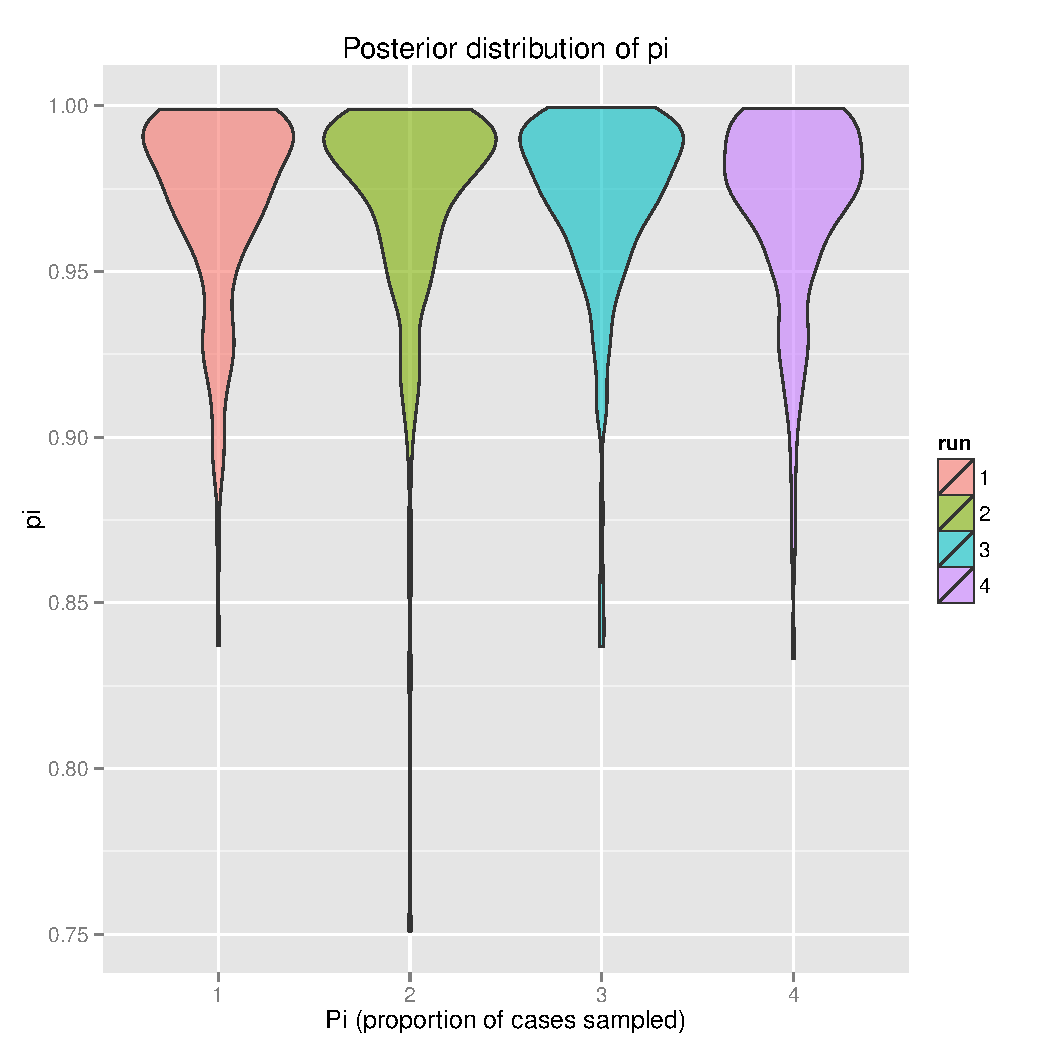
\includegraphics[width=.6\textwidth]{figs/unnamed-chunk-41} 

}



\end{knitrout}


\begin{knitrout}
\definecolor{shadecolor}{rgb}{0.969, 0.969, 0.969}\color{fgcolor}\begin{kframe}
\begin{alltt}
\hlstd{x} \hlkwb{<-} \hlkwd{data.frame}\hlstd{(}\hlkwc{date}\hlstd{=}\hlkwd{as.vector}\hlstd{(}\hlkwd{row}\hlstd{(incid)),}
                \hlkwc{step}\hlstd{=}\hlkwd{as.vector}\hlstd{(}\hlkwd{col}\hlstd{(incid)),}
                \hlkwc{incidence}\hlstd{=}\hlkwd{as.vector}\hlstd{(incid))}
\hlkwd{head}\hlstd{(x)}
\end{alltt}
\begin{verbatim}
##   date step incidence
## 1    1    1         1
## 2    2    1         0
## 3    3    1         1
## 4    4    1         2
## 5    5    1         2
## 6    6    1         1
\end{verbatim}
\begin{alltt}
\hlstd{p} \hlkwb{<-} \hlkwd{ggplot}\hlstd{(}\hlkwc{data}\hlstd{=x,} \hlkwd{aes}\hlstd{(}\hlkwc{x}\hlstd{=date,} \hlkwc{y}\hlstd{=incidence))} \hlopt{+} \hlkwd{labs}\hlstd{(}\hlkwc{title}\hlstd{=}\hlstr{"Posterior estimates of incidence"}\hlstd{)}
\end{alltt}
\end{kframe}
\end{knitrout}



\begin{knitrout}
\definecolor{shadecolor}{rgb}{0.969, 0.969, 0.969}\color{fgcolor}\begin{kframe}
\begin{alltt}
\hlstd{p} \hlopt{+} \hlkwd{geom_boxplot}\hlstd{(}\hlkwd{aes}\hlstd{(}\hlkwc{x}\hlstd{=}\hlkwd{factor}\hlstd{(date)))}
\end{alltt}
\end{kframe}

{\centering 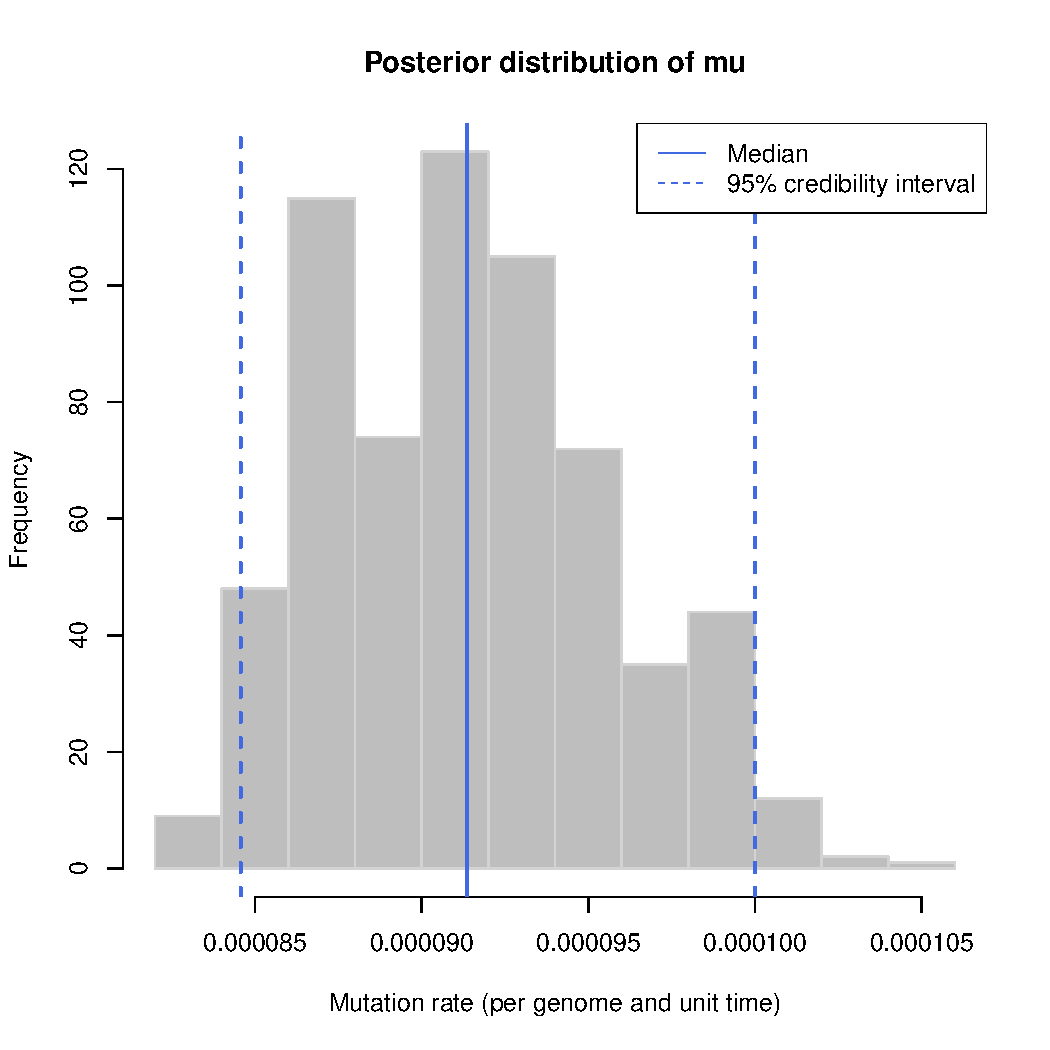
\includegraphics[width=.6\textwidth]{figs/unnamed-chunk-43} 

}



\end{knitrout}


\begin{knitrout}
\definecolor{shadecolor}{rgb}{0.969, 0.969, 0.969}\color{fgcolor}\begin{kframe}
\begin{alltt}
\hlstd{p} \hlopt{+} \hlkwd{geom_jitter}\hlstd{(}\hlkwd{aes}\hlstd{(}\hlkwc{x}\hlstd{=}\hlkwd{factor}\hlstd{(date)),} \hlkwc{alpha}\hlstd{=}\hlnum{.2}\hlstd{)}
\end{alltt}
\end{kframe}

{\centering 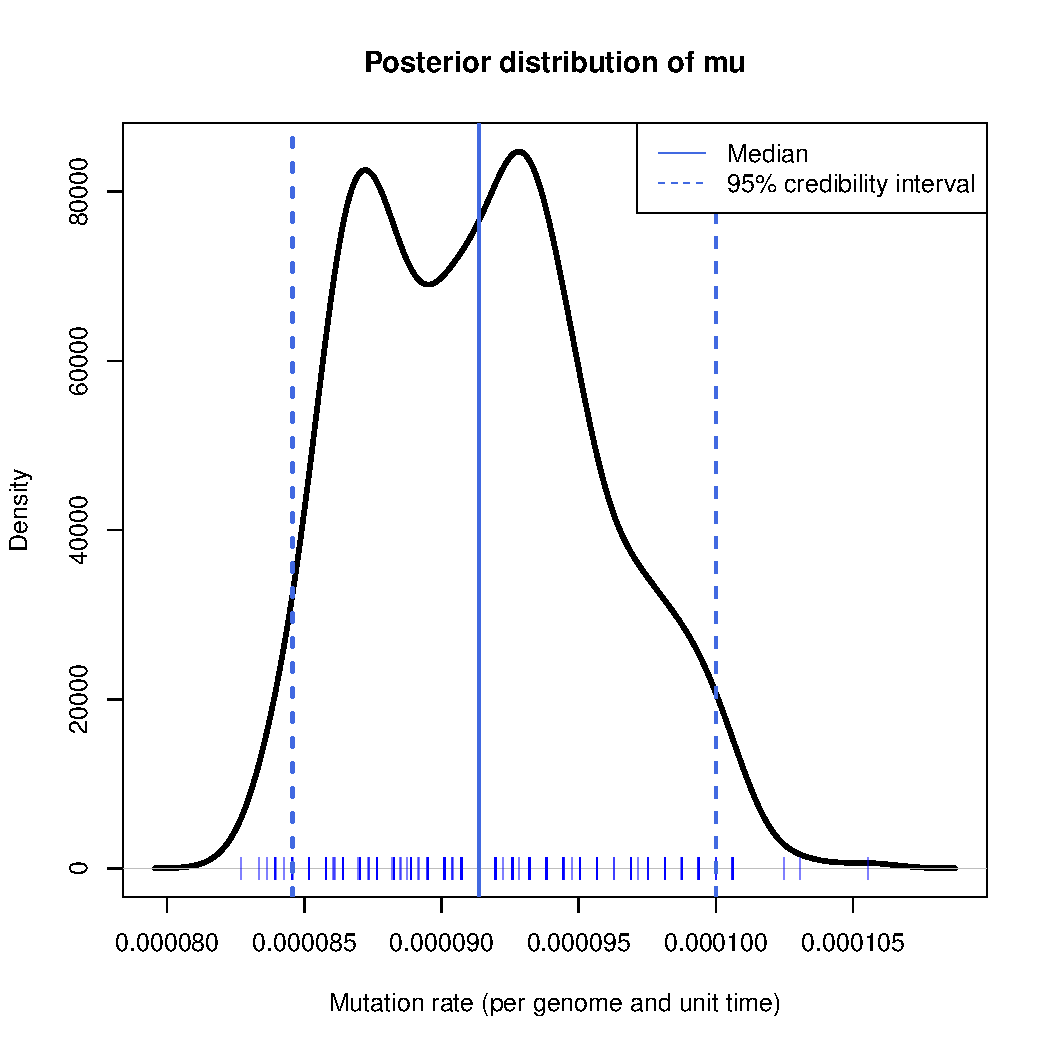
\includegraphics[width=.6\textwidth]{figs/unnamed-chunk-44} 

}



\end{knitrout}


\begin{knitrout}
\definecolor{shadecolor}{rgb}{0.969, 0.969, 0.969}\color{fgcolor}\begin{kframe}
\begin{alltt}
\hlstd{p} \hlopt{+} \hlkwd{geom_jitter}\hlstd{(}\hlkwc{alpha}\hlstd{=}\hlnum{.1}\hlstd{)} \hlopt{+} \hlkwd{geom_smooth}\hlstd{(}\hlkwc{method}\hlstd{=lm,} \hlkwc{formula}\hlstd{=y}\hlopt{~}\hlkwd{ns}\hlstd{(x,}\hlnum{10}\hlstd{),} \hlkwc{size}\hlstd{=}\hlnum{1}\hlstd{)}
\end{alltt}
\end{kframe}

{\centering 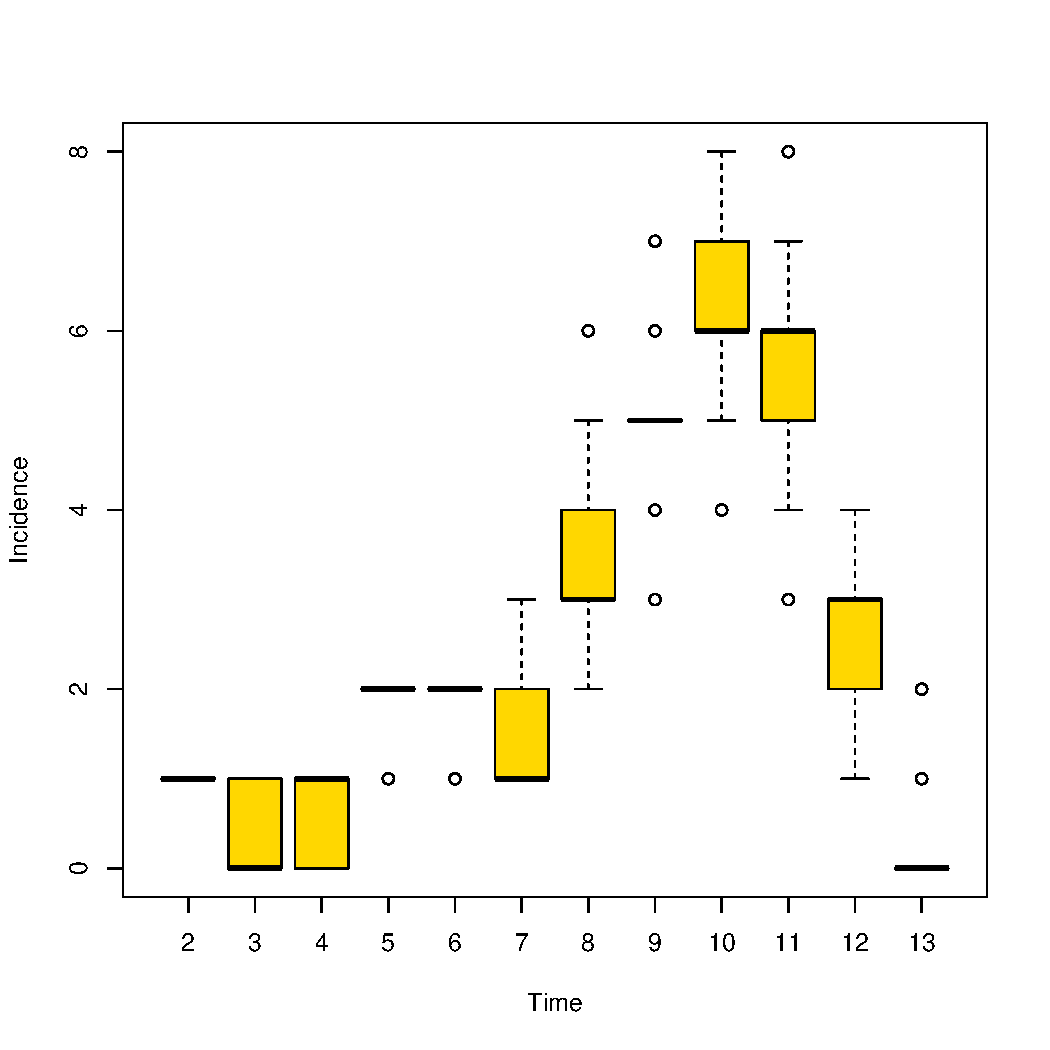
\includegraphics[width=.6\textwidth]{figs/unnamed-chunk-45} 

}



\end{knitrout}



\begin{knitrout}
\definecolor{shadecolor}{rgb}{0.969, 0.969, 0.969}\color{fgcolor}\begin{kframe}
\begin{alltt}
\hlstd{p} \hlopt{+} \hlkwd{geom_bin2d}\hlstd{()}
\end{alltt}
\end{kframe}

{\centering 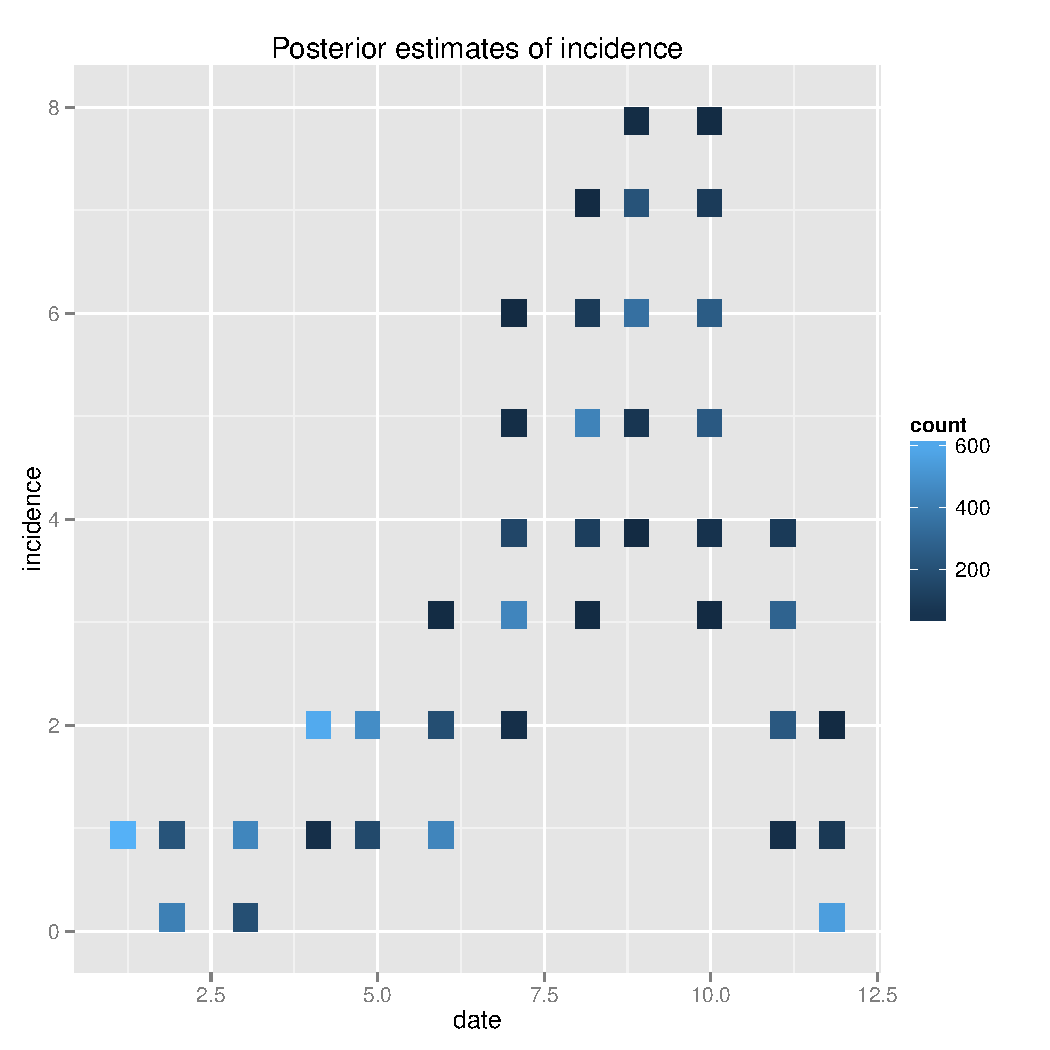
\includegraphics[width=.6\textwidth]{figs/unnamed-chunk-461} 

}


\begin{kframe}\begin{alltt}
\hlstd{p} \hlopt{+} \hlkwd{geom_bin2d}\hlstd{(}\hlkwc{binwidth}\hlstd{=}\hlkwd{c}\hlstd{(}\hlnum{1}\hlstd{,}\hlnum{1}\hlstd{))}
\end{alltt}
\end{kframe}

{\centering 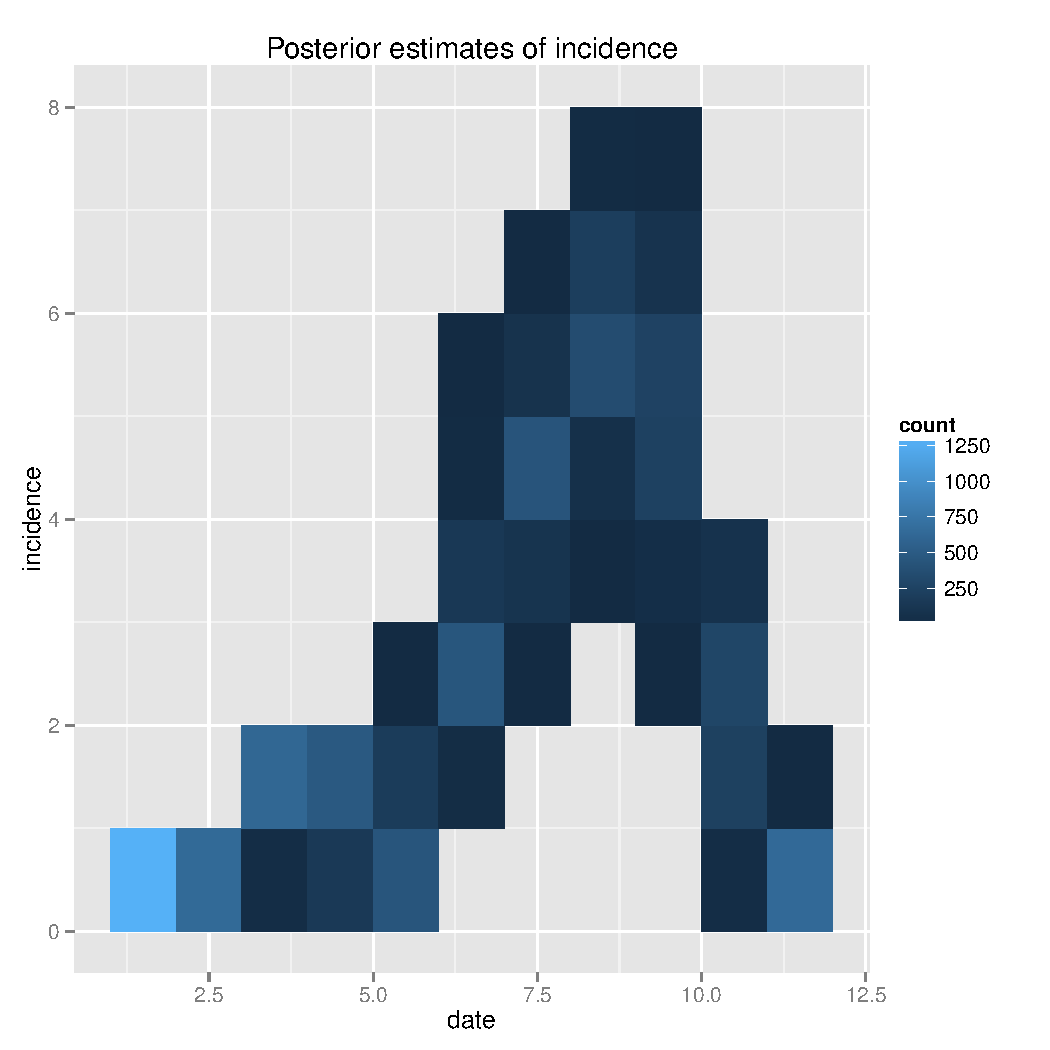
\includegraphics[width=.6\textwidth]{figs/unnamed-chunk-462} 

}



\end{knitrout}


\begin{knitrout}
\definecolor{shadecolor}{rgb}{0.969, 0.969, 0.969}\color{fgcolor}\begin{kframe}
\begin{alltt}
\hlstd{p} \hlopt{+} \hlkwd{geom_hex}\hlstd{(}\hlkwc{bins}\hlstd{=}\hlnum{8}\hlstd{)}
\end{alltt}
\end{kframe}

{\centering 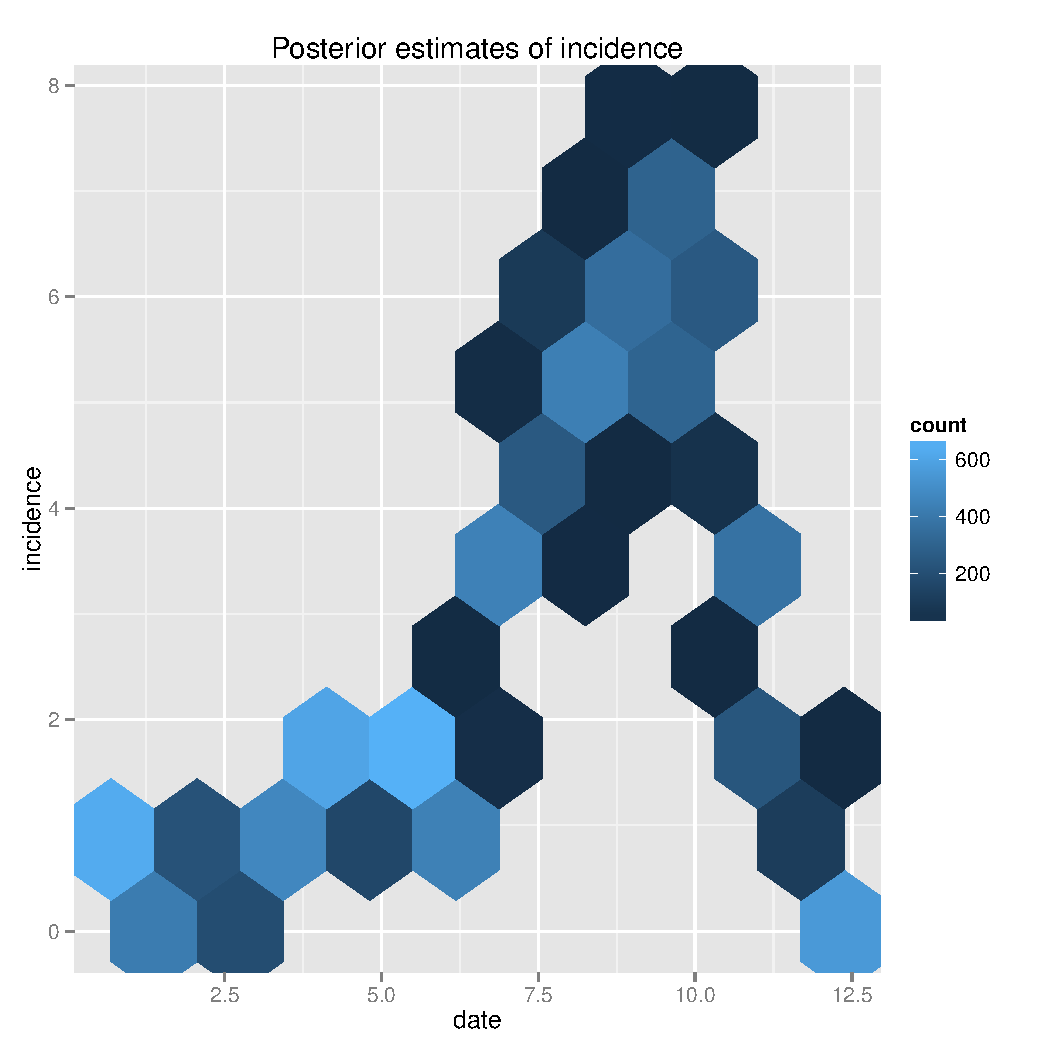
\includegraphics[width=.6\textwidth]{figs/unnamed-chunk-47} 

}



\end{knitrout}





\begin{knitrout}
\definecolor{shadecolor}{rgb}{0.969, 0.969, 0.969}\color{fgcolor}\begin{kframe}
\begin{alltt}
\hlstd{R} \hlkwb{<-} \hlkwd{get.R}\hlstd{(res)}
\hlkwd{dim}\hlstd{(R)}
\end{alltt}
\begin{verbatim}
## [1] 640  30
\end{verbatim}
\begin{alltt}
\hlkwd{barplot}\hlstd{(}\hlkwd{table}\hlstd{(R)}\hlopt{/}\hlkwd{length}\hlstd{(R),} \hlkwc{xlab}\hlstd{=}\hlstr{"Number of secondary cases"}\hlstd{,} \hlkwc{main}\hlstd{=}\hlstr{"Posterior estimates of effective reproduction numbers (R)"}\hlstd{,} \hlkwc{ylab}\hlstd{=}\hlstr{"Frequency"}\hlstd{)}
\end{alltt}
\end{kframe}

{\centering 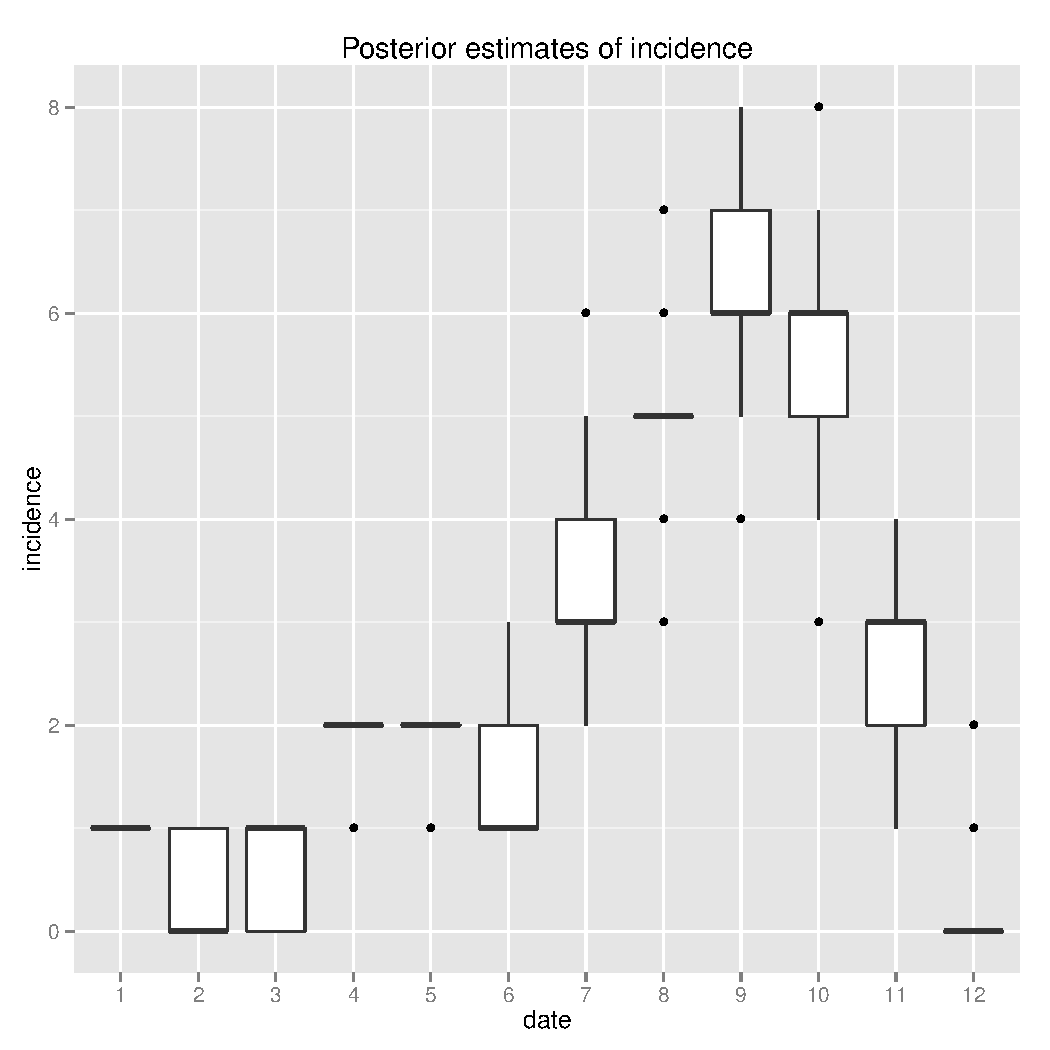
\includegraphics[width=.6\textwidth]{figs/unnamed-chunk-48} 

}



\end{knitrout}


\begin{knitrout}
\definecolor{shadecolor}{rgb}{0.969, 0.969, 0.969}\color{fgcolor}\begin{kframe}
\begin{alltt}
\hlstd{x} \hlkwb{<-} \hlkwd{data.frame}\hlstd{(}\hlkwc{case}\hlstd{=}\hlkwd{factor}\hlstd{(}\hlkwd{as.vector}\hlstd{(}\hlkwd{col}\hlstd{(R)),} \hlkwc{levels}\hlstd{=}\hlkwd{as.character}\hlstd{(}\hlnum{1}\hlopt{:}\hlnum{30}\hlstd{)),}\hlkwc{R}\hlstd{=}\hlkwd{as.vector}\hlstd{(R))}
\hlkwd{head}\hlstd{(x)}
\end{alltt}
\begin{verbatim}
##   case R
## 1    1 1
## 2    1 1
## 3    1 1
## 4    1 1
## 5    1 1
## 6    1 1
\end{verbatim}
\begin{alltt}
\hlkwd{tail}\hlstd{(x)}
\end{alltt}
\begin{verbatim}
##       case R
## 19195   30 0
## 19196   30 0
## 19197   30 0
## 19198   30 0
## 19199   30 0
## 19200   30 0
\end{verbatim}
\end{kframe}
\end{knitrout}



\begin{knitrout}
\definecolor{shadecolor}{rgb}{0.969, 0.969, 0.969}\color{fgcolor}\begin{kframe}
\begin{alltt}
\hlstd{p} \hlkwb{<-} \hlkwd{ggplot}\hlstd{(}\hlkwc{data}\hlstd{=x,} \hlkwd{aes}\hlstd{(}\hlkwc{x}\hlstd{=case,} \hlkwc{y}\hlstd{=R))} \hlopt{+} \hlkwd{labs}\hlstd{(}\hlkwc{title}\hlstd{=}\hlstr{"Posterior estimates of effective reproduction numbers"}\hlstd{)}
\hlstd{p} \hlopt{+} \hlkwd{geom_boxplot}\hlstd{()}
\end{alltt}
\end{kframe}

{\centering 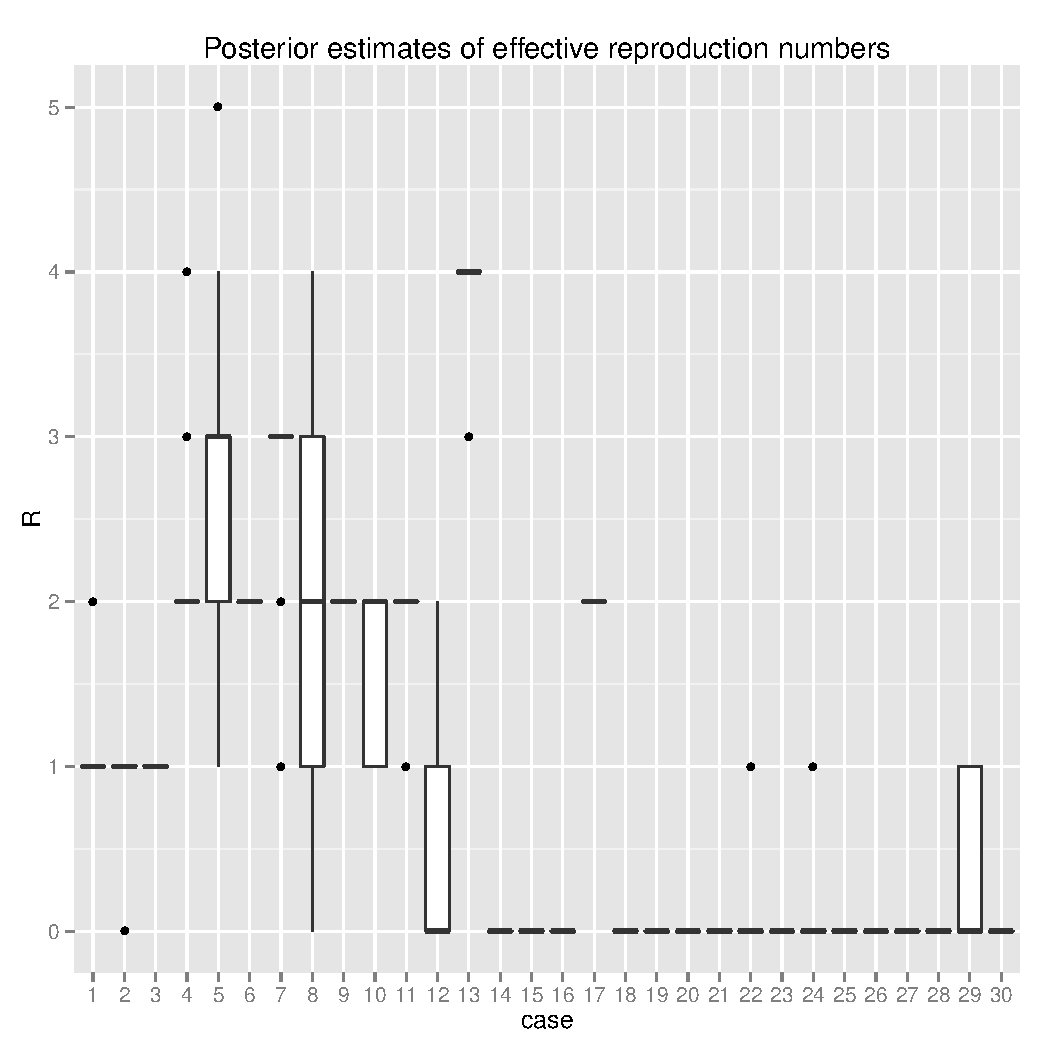
\includegraphics[width=.6\textwidth]{figs/unnamed-chunk-501} 

}


\begin{kframe}\begin{alltt}
\hlstd{p} \hlopt{+} \hlkwd{geom_boxplot}\hlstd{(}\hlkwd{aes}\hlstd{(}\hlkwc{colour}\hlstd{=case))}
\end{alltt}
\end{kframe}

{\centering 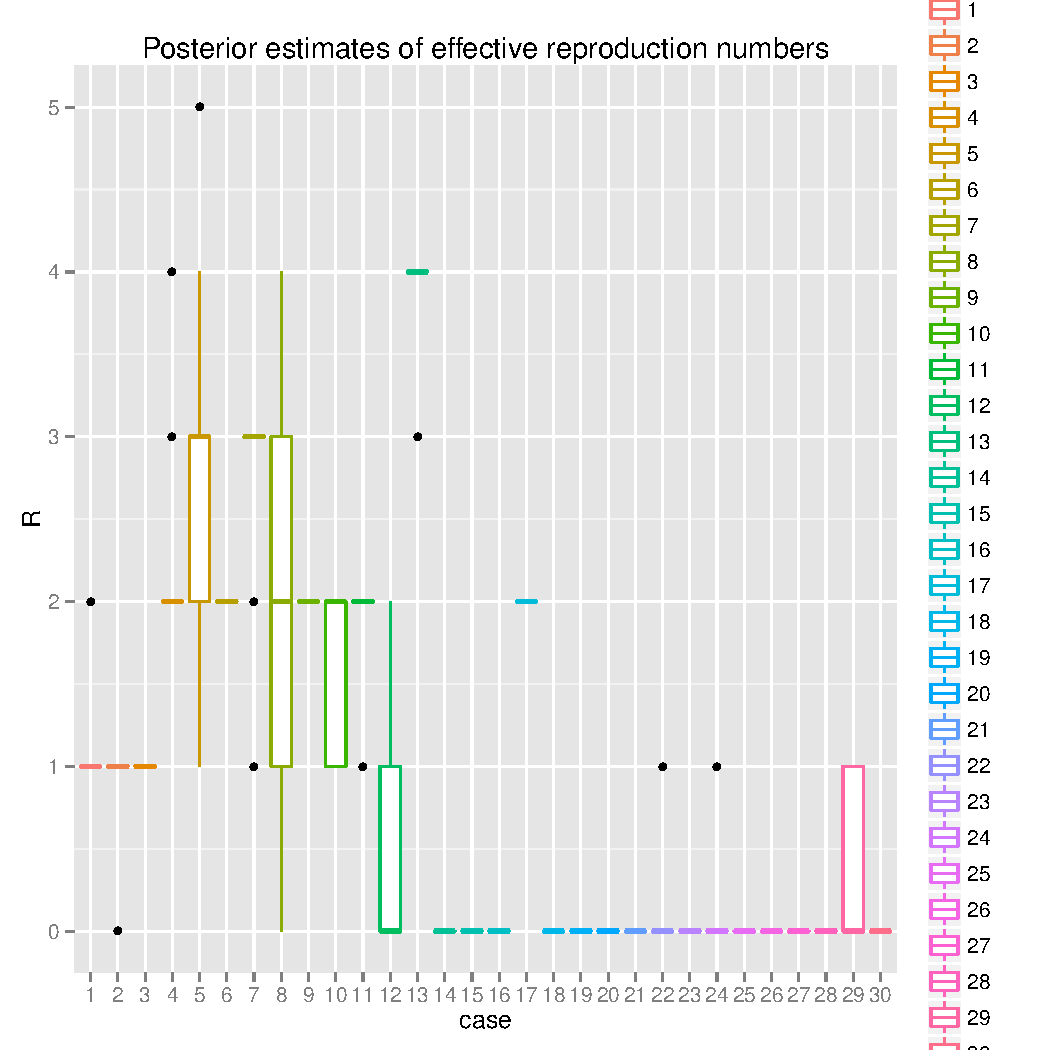
\includegraphics[width=.6\textwidth]{figs/unnamed-chunk-502} 

}



\end{knitrout}






%% %%%%%%%%%%%%%%%%%%%%%%%%%%%%%%%%%%%%%%%%%%%%%%%%%%%%
%% %%%%%%%%%%%%%%%%%%%%%%%%%%%%%%%%%%%%%%%%%%%%%%%%%%%%
%% \section{Advanced uses}
%% %%%%%%%%%%%%%%%%%%%%%%%%%%%%%%%%%%%%%%%%%%%%%%%%%%%%
%% %%%%%%%%%%%%%%%%%%%%%%%%%%%%%%%%%%%%%%%%%%%%%%%%%%%%



%% %%%%%%%%%%%%%%%%%%%%%%%%%%%%%%%%%%%%%%%%%%%%%%%%%%%%
%% \subsection{Fixing known ancestries}
%% %%%%%%%%%%%%%%%%%%%%%%%%%%%%%%%%%%%%%%%%%%%%%%%%%%%%



\end{document}
